\documentclass[a4paper]{article}

\usepackage{inputenc}
% \usepackage[british,UKenglish]{babel}
\usepackage{xeCJK}
\usepackage{amsmath,amsthm,amsfonts,amssymb,amscd,bm,arydshln}
\usepackage{mathtools}
\usepackage{physics}
\usepackage{mathrsfs}

%\usepackage{titlesec}
\usepackage{color}
\usepackage{graphicx}
\usepackage{fancyref}
\usepackage{hyperref}
\usepackage{float}
% \usepackage{scrextend}
\usepackage{setspace}
\usepackage{xargs}
\usepackage{multicol}
\usepackage{nameref}
\usepackage{subfigure}

\usepackage{sectsty}
\usepackage{multicol}
\usepackage{multirow}
\usepackage[procnames]{listings}
\usepackage{appendix}
\usepackage{listings}

\usepackage{fullpage}
\usepackage[top=2cm, bottom=4.5cm, left=2.5cm, right=2.5cm]{geometry}

\newcommand\tab[1][1cm]{\hspace*{#1}}
\hypersetup{colorlinks=true, linkcolor=black}
\interfootnotelinepenalty=10000

\newcommand{\cleancode}[1]{\begin{addmargin}[3em]{3em}\texttt{\textcolor{cleanOrange}{#1}}\end{addmargin}}
\newcommand{\cleanstyle}[1]{\text{\textcolor{cleanOrange}{\texttt{#1}}}}

\usepackage[colorinlistoftodos,prependcaption,textsize=footnotesize]{todonotes}
\newcommandx{\commred}[2][1=]{\textcolor{Red}
{\todo[linecolor=red,backgroundcolor=red!25,bordercolor=red,#1]{#2}}}
\newcommandx{\commblue}[2][1=]{\textcolor{Blue}
{\todo[linecolor=blue,backgroundcolor=blue!25,bordercolor=blue,#1]{#2}}}
\newcommandx{\commgreen}[2][1=]{\textcolor{OliveGreen}{\todo[linecolor=OliveGreen,backgroundcolor=OliveGreen!25,bordercolor=OliveGreen,#1]{#2}}}
\newcommandx{\commpurp}[2][1=]{\textcolor{Plum}{\todo[linecolor=Plum,backgroundcolor=Plum!25,bordercolor=Plum,#1]{#2}}}

\def\code#1{{\tt #1}}

\def\note#1{\noindent{\bf [Note: #1]}}

\makeatletter
%% The "\@seccntformat" command is an auxiliary command
%% (see pp. 26f. of 'The LaTeX Companion,' 2nd. ed.)
\def\@seccntformat#1{\@ifundefined{#1@cntformat}%
   {\csname the#1\endcsname\quad}  % default
   {\csname #1@cntformat\endcsname}% enable individual control
}
\let\oldappendix\appendix %% save current definition of \appendix
\renewcommand\appendix{%
    \oldappendix
    \newcommand{\section@cntformat}{\appendixname~\thesection\quad}
}
\makeatother



\usepackage{pythonhighlight}

% \lstset{frame=, basicstyle={\footnotesize\ttfamily}}
\graphicspath{ {images/} }


%-----------------------------------------BEGIN DOC----------------------------------------

\begin{document}
\renewcommand{\contentsname}{目\ 录}
\renewcommand{\appendixname}{附录}
\renewcommand{\appendixpagename}{附录}
\renewcommand{\refname}{参考文献} 
\renewcommand{\figurename}{图}
\renewcommand{\tablename}{表}
\renewcommand{\today}{\number\year 年 \number\month 月 \number\day 日}


\title{\vspace{6.0cm}{\Huge Mini Project{\large\linebreak\\}}{\Large CSE5002智能数据分析\linebreak\linebreak}}
%please write your name, Student #, and Class # in Authors, student ID, and class # respectively
\author{
\begin{tabular}{rl}
    姓名: & 李子强  \\
    学号: & 11930674
\end{tabular}
}
\date{\today}
\maketitle
\newpage

%-----------------------------------------CONTENT-------------------------------------
\begin{center}
\tableofcontents\label{c}
\end{center}
\newpage

%------------------------------------------TEXT--------------------------------------------

\section{数据预处理}

\subsection{数据描述}

\begin{figure}[!h]
  \subfigure[训练集]{ 
    \label{fig:label-dist:train}
    \begin{minipage}[b]{0.47\textwidth} 
      \centering 
      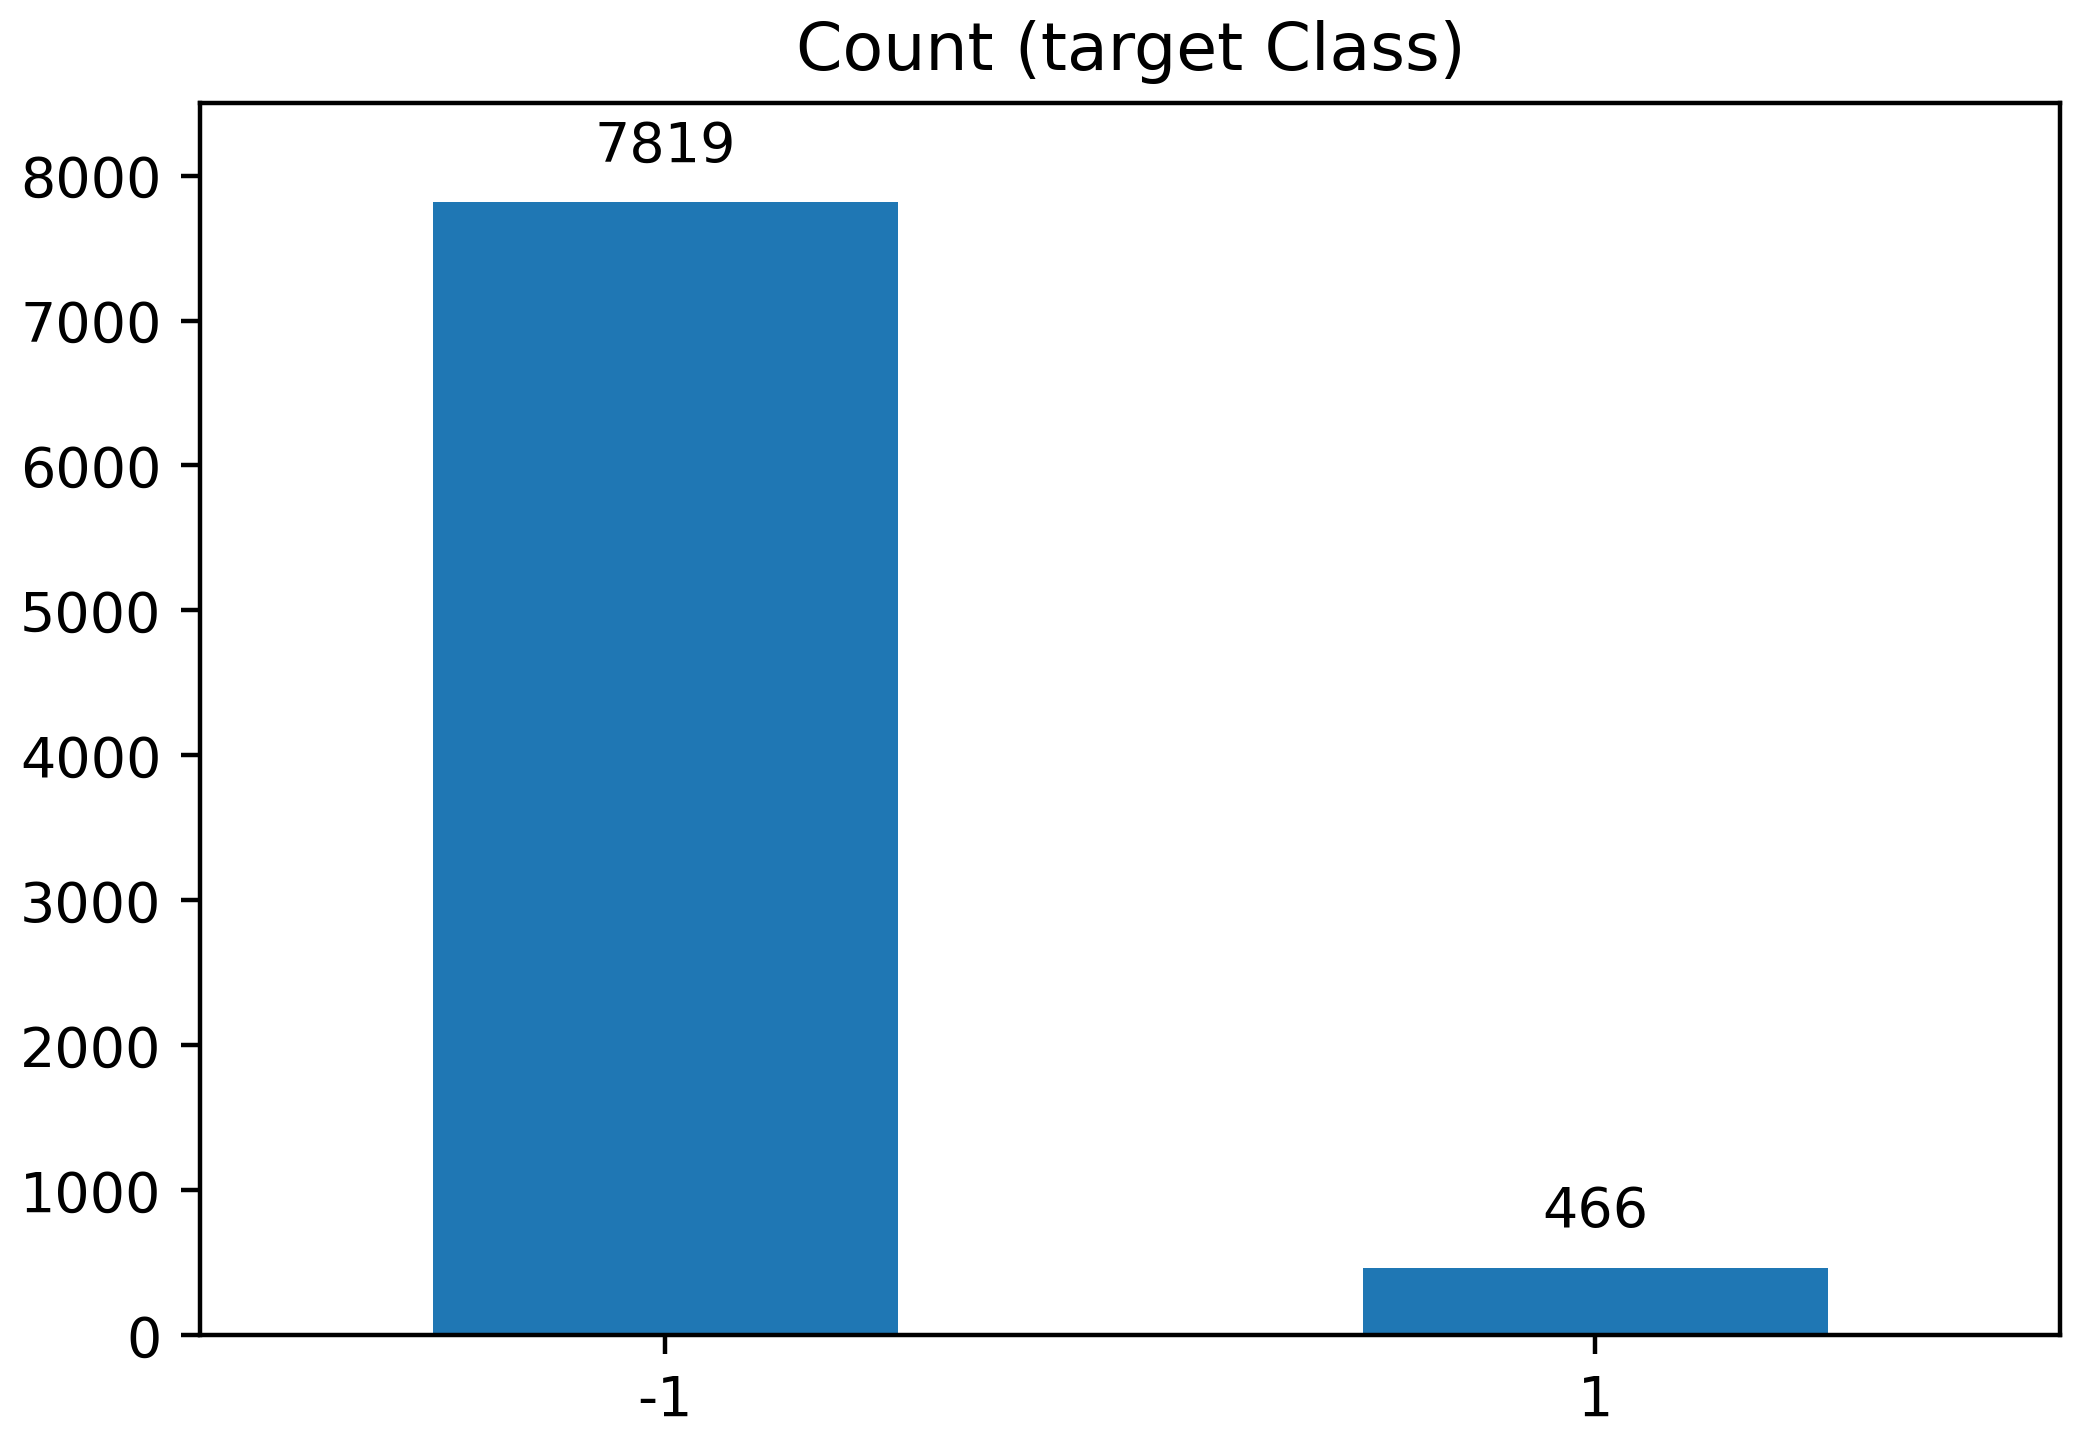
\includegraphics[width=\linewidth]{train_dist.png} 
    \end{minipage}}% 
  \subfigure[测试集]{ 
    \label{fig:label-dist:test}
    \begin{minipage}[b]{0.47\textwidth} 
      \centering 
      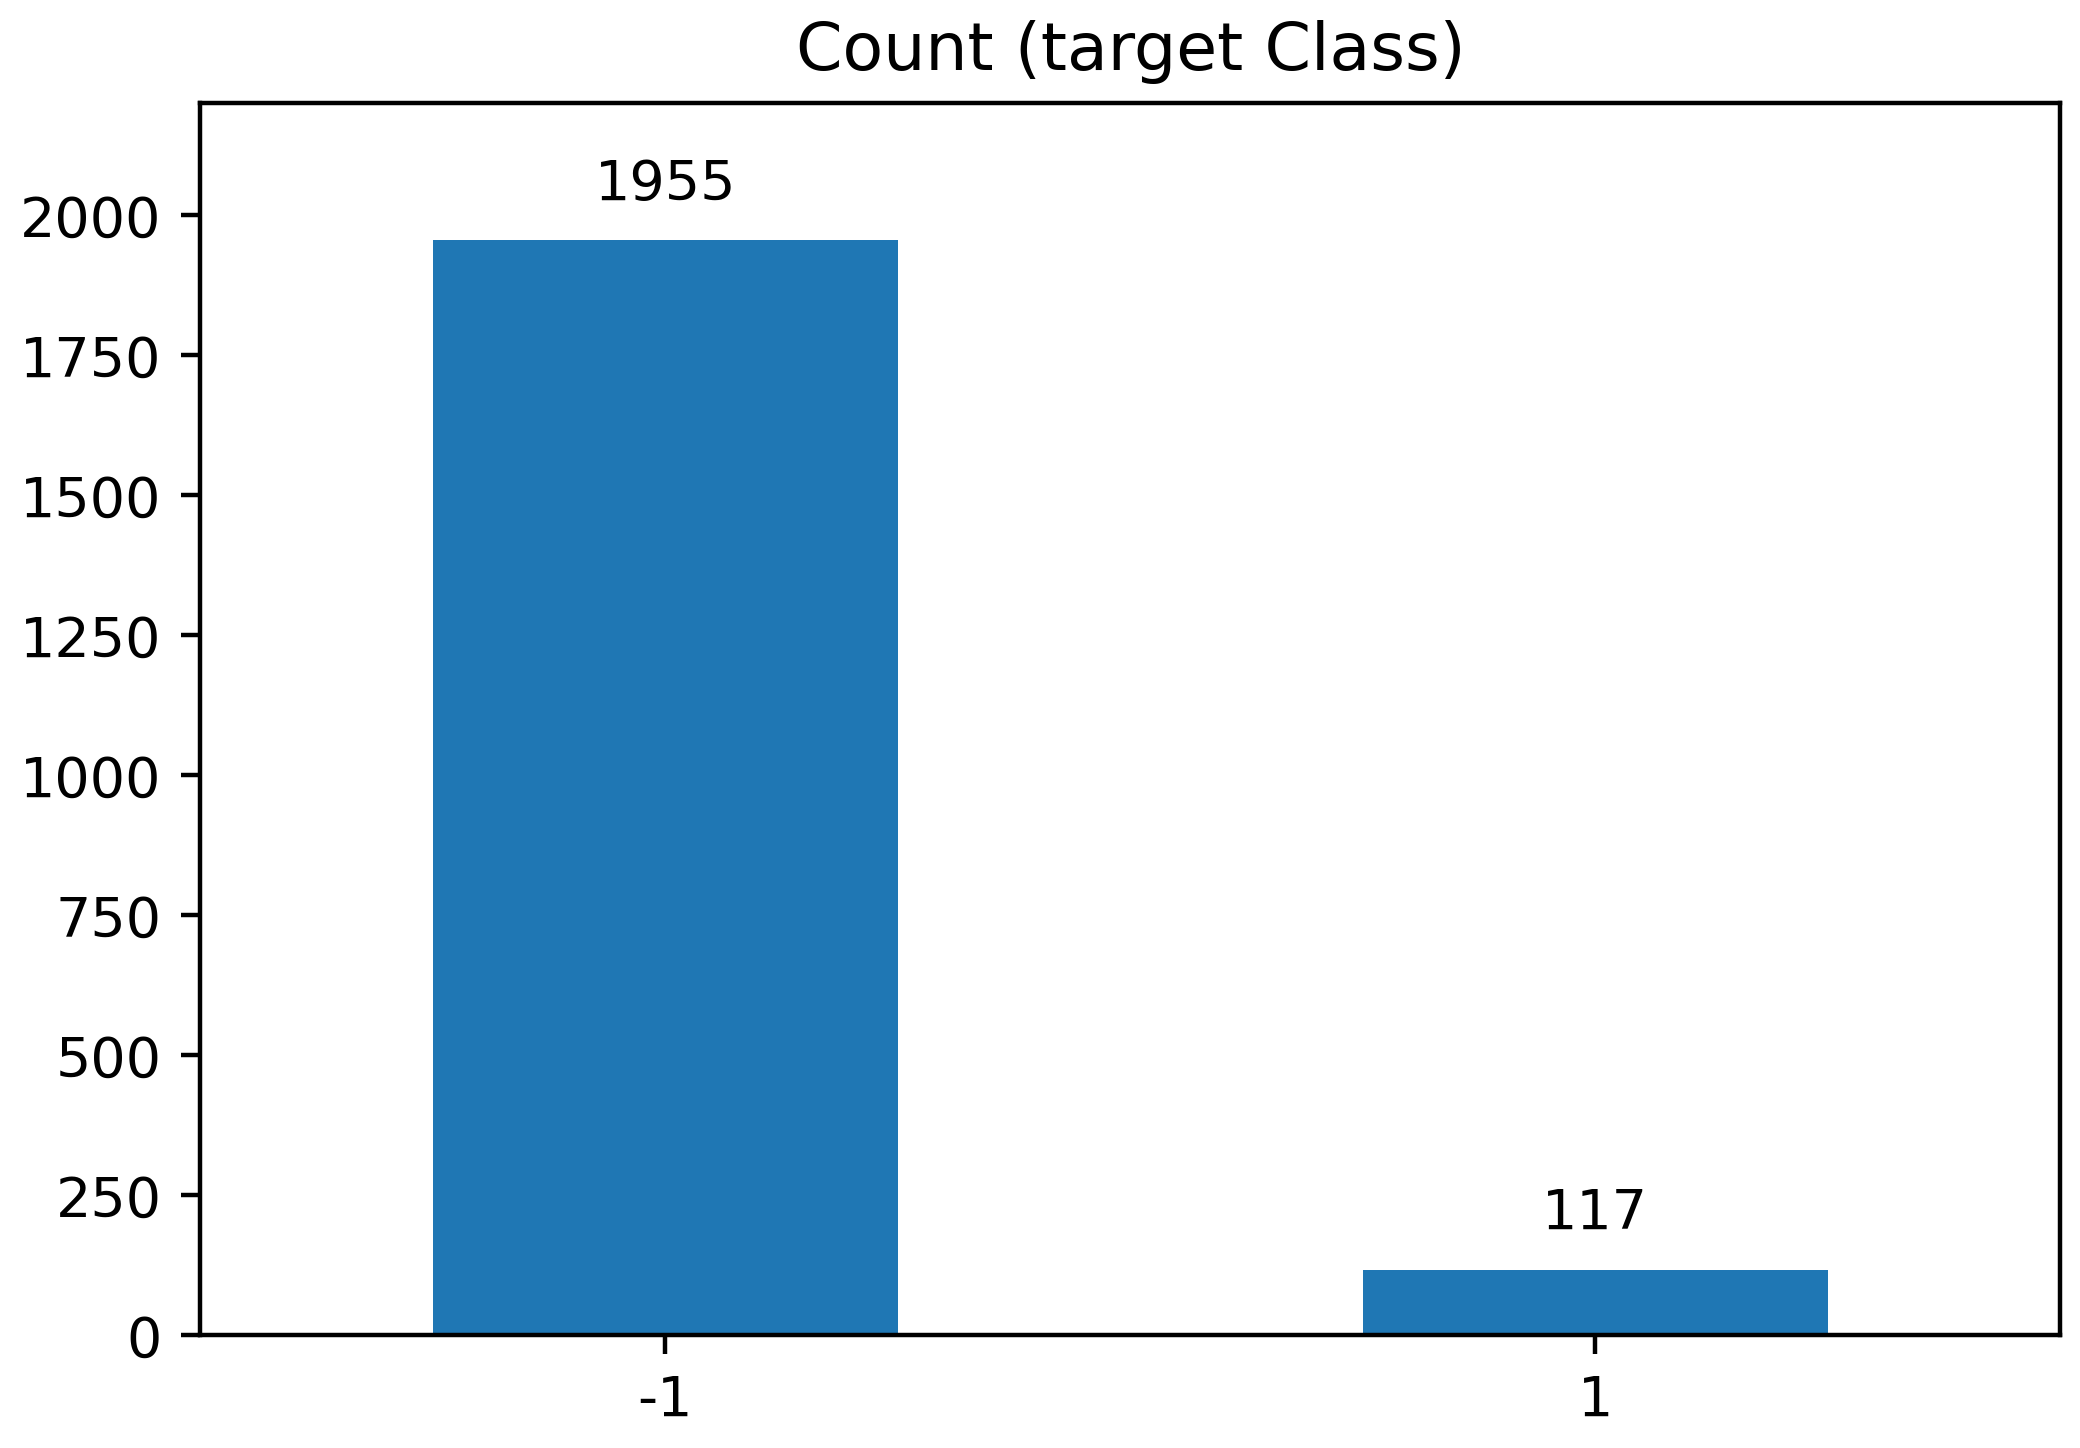
\includegraphics[width=\linewidth]{test_dist.png} 
    \end{minipage}} 
  \caption{标签分布} 
  \label{fig:label-dist} %% label for entire figure 
\end{figure}

如图\ref{fig:label-dist}所示,这是一个二分类问题。在训练集中,负类(7819)和正类(466)比例悬殊,
比例达 16.78 比 1。如果直接全部标记为负类准确度也能达到 94.38\%。所以对数据集采样的时候,一定需要考虑样本量平衡处理的问题。

\subsection{特征相关性分析}

\begin{figure}[!h]
    \centering
    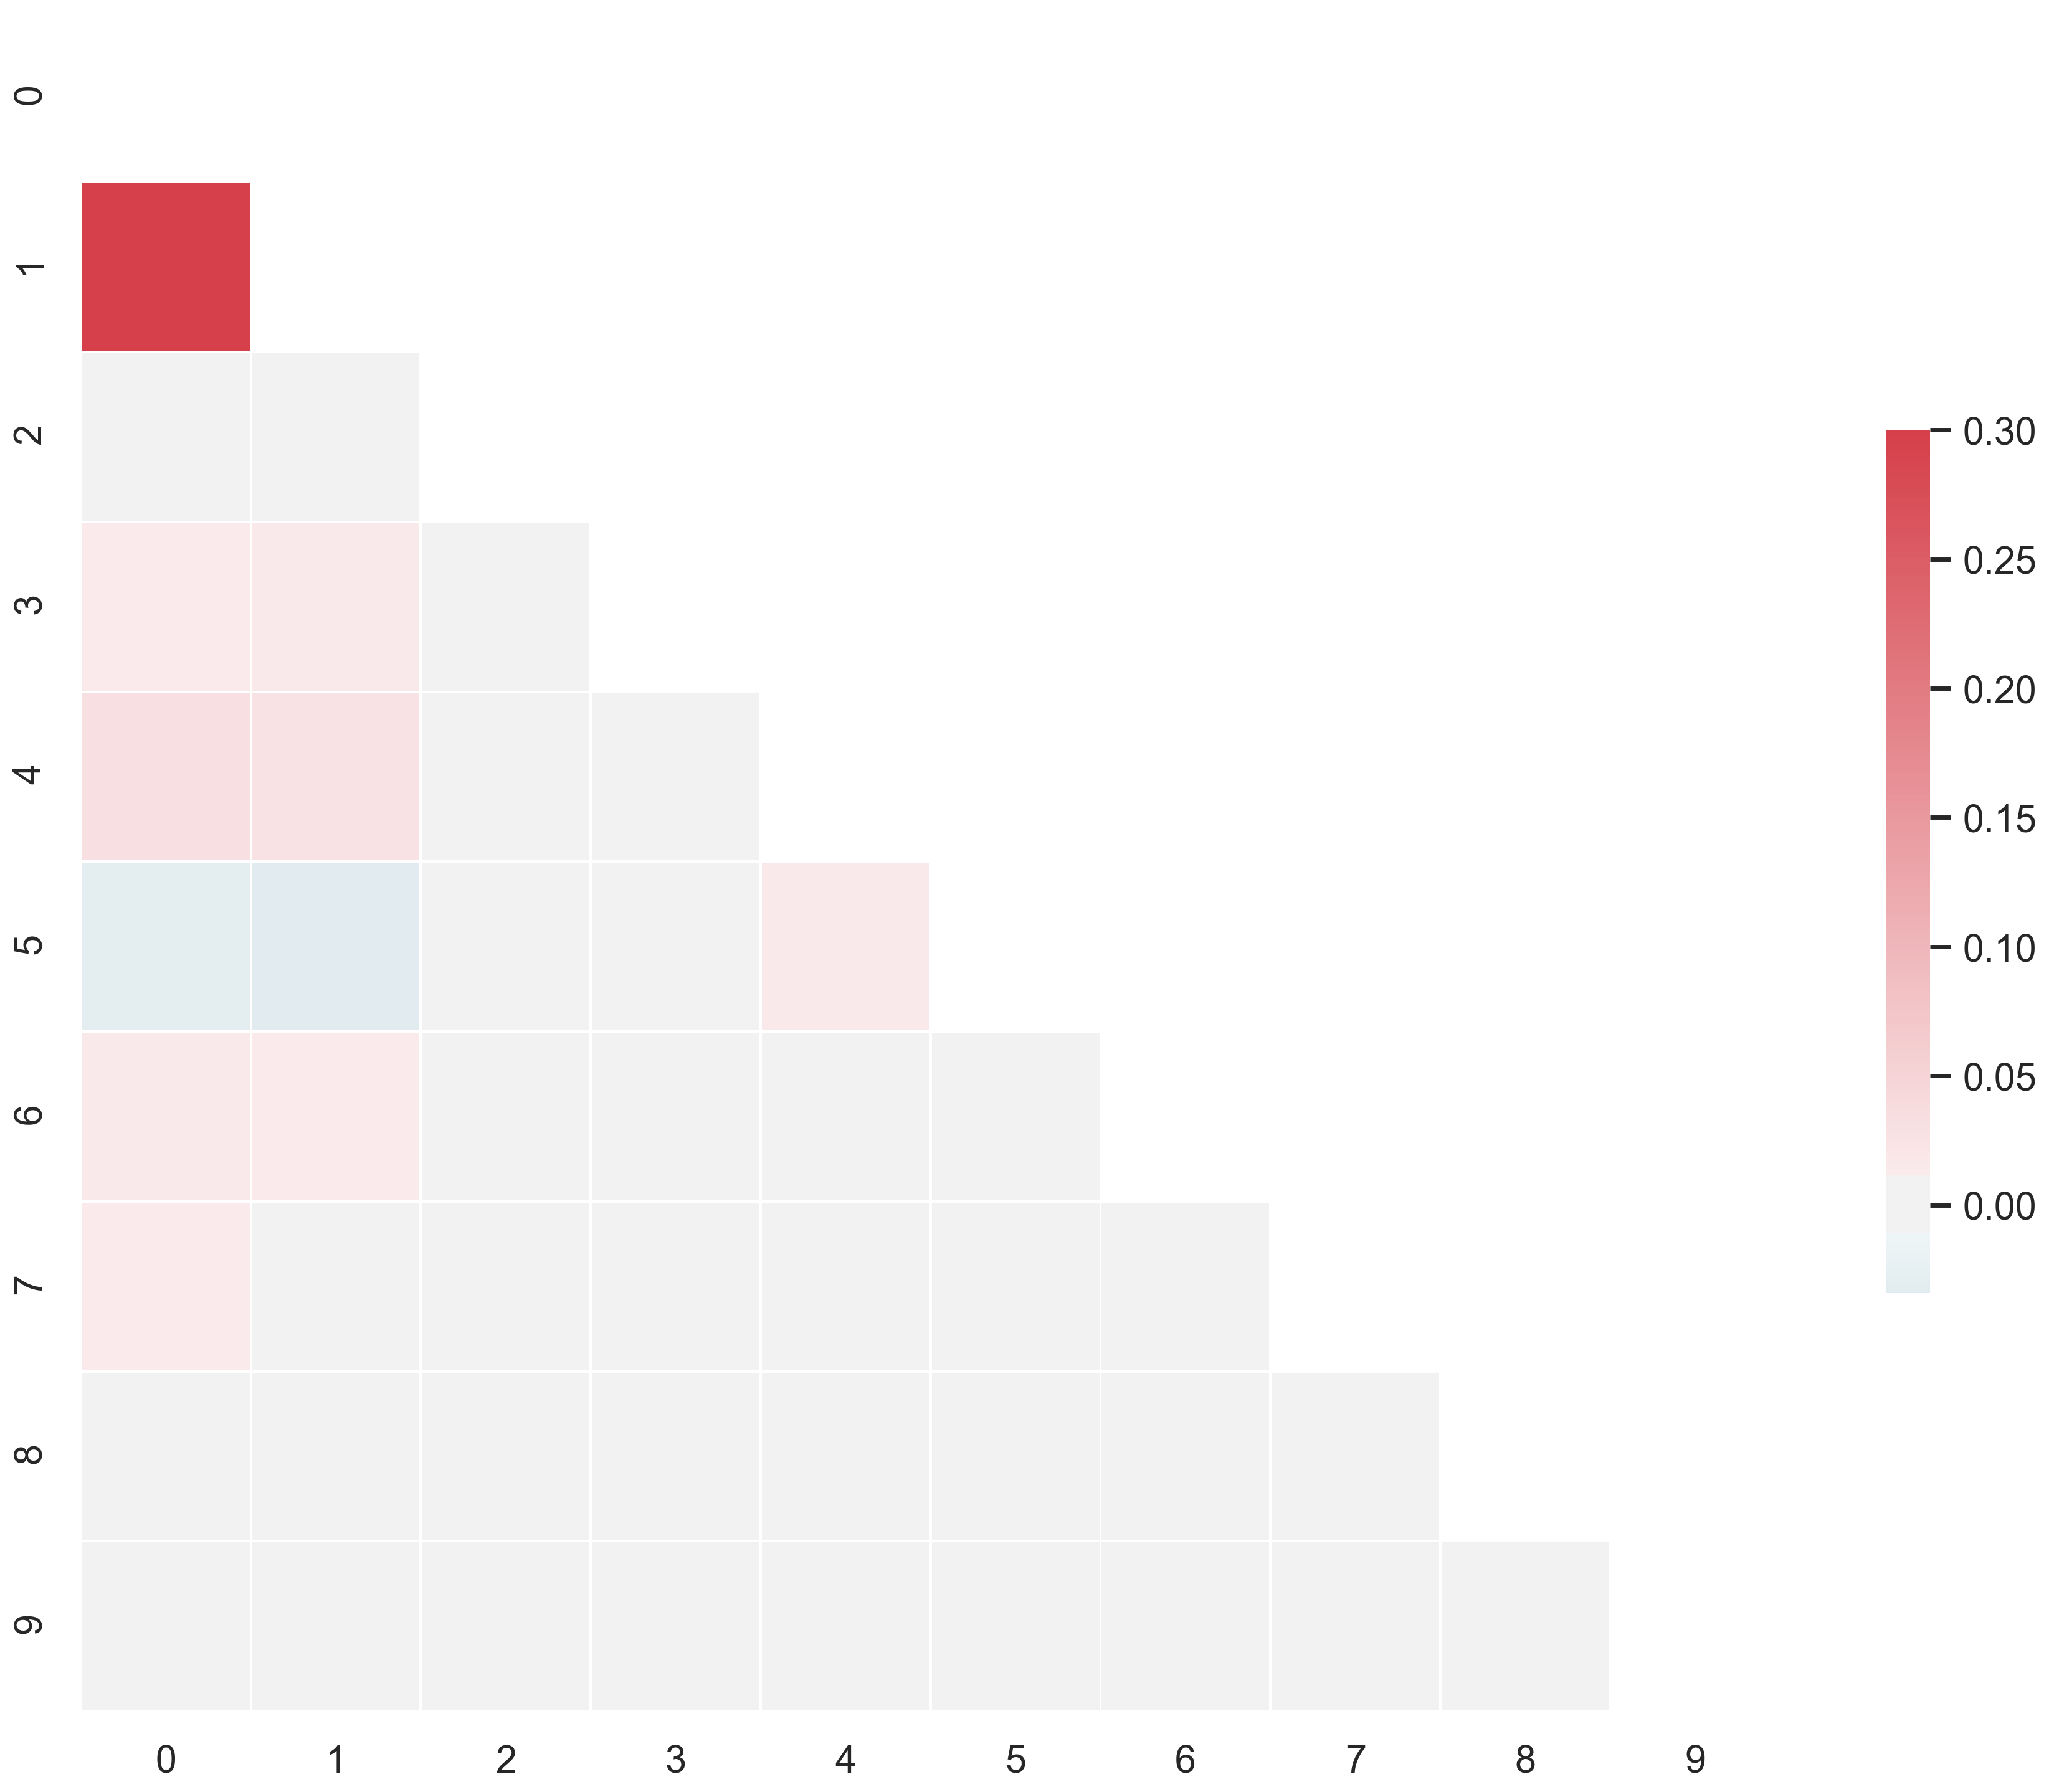
\includegraphics[width=0.6\linewidth]{train_corr2.png}
    \caption{训练集的相关性矩阵}
    \label{fig:corr}
\end{figure}

数据集共有10个维度,使用皮尔逊相关系数分析两两特征之间的相关关系,画出图\ref{fig:corr}。皮尔逊相关系数绝对值趋近于0,两个随机变量趋于无关;绝对值趋近于1趋于相关。相关系数大于0为正相关,小于0为负相关。可以看出比较多特征之间是没有关系的,但是,第0维和第1维是强相关。

\subsection{采样}

通常非平衡数据的处理方式是欠采样(under-sampling)和过采样(oversampling)。欠采样是丢弃多数类的数据,因为只学习了一部分数据,可能会造成偏差增加,造成过拟合。过采样是重复或者合成少数类数据,实际上没有为模型引入更多数据,过分强调少数类数据,会放大少数类噪音对模型的影响。

SMOTE (Synthetic Minority Oversampling Technique) 是2002年Chawla等人提出的一种在随机采样的基础上改进的一种过采样算法\cite{Chawla2002SMOTE}。基本思想就是对少数类别样本进行分析和模拟,并将人工模拟的新样本添加到数据集中,进而使原始数据中的类别不再严重失衡。该算法的模拟过程采用了K最近邻(kNN,k-NearestNeighbor),模拟生成新样本的步骤:
\begin{enumerate}
    \item 采样最邻近算法,计算出每个少数类样本$\tilde{x}$的K个近邻$\tilde{x}_i$;
    \item 从K个近邻中随机挑选N个样本进行随机线性插值;
    \item 构造新的少数类样本 $x_{new}=x+rand\left(0,1\right)\times\left(\tilde{x}-\tilde{x}_i   \right)$;
    \item 将新样本与原数据合成,产生新的数据集;
\end{enumerate}
\begin{figure}[!h]
    \centering
    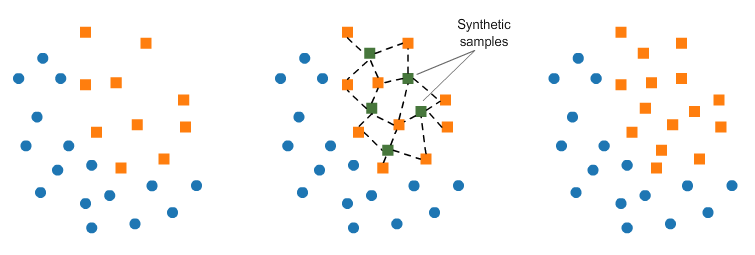
\includegraphics[width=0.7\linewidth]{smote.png}
    \caption{SMOTE生成示例}
    \label{fig:smote}
\end{figure}

\todo{使用过采样(或SMOTE)+强正则模型(如XGBoost)可能比较适合不平衡的数据。拿到一个新的数据时,可以不妨直接先试试这个方法,作为基准(Baseline)}

除此之外,还有由SMOTE衍生出来的变体算法,比如:Border-line SMOTE。

另外,ADASYN (Adaptive Synthetic) 
是 2008年 He 等人提出的一种自适应综合过采样方法\cite{he2008adasyn}。
其最大的特点是采用某种机制自动决定每个少数类样本需要产生多少合成样本,而不是像SMOTE那样对每个少数类样本合成同数量的样本。具体流程如下:

首先计算需要合成的样本总量:
\[ G = (S_{maj} - S_{min}) \times \beta \]
其中\(S_{maj}\)为多数类样本数量,\(S_{min}\)为少数类样本数量,\(\beta \in [0,1]\)为系数。$G$即为总共想要合成的少数类样本数量,如果\(\beta=1\)则是合成后各类别数目相等。
​

对于每个少类别样本\(\mathbf{x}_i\),找出其K近邻个点,并计算:
\[ \Gamma_i = \frac{\Delta_i\,/\,K}{Z} \]
其中\(\Delta_i\)为K近邻个点中多数类样本的数量,Z为规范化因子以确保 \(\Gamma\) 构成一个分布。这样若一个少数类样本\(\mathbf{x}_i\)的周围多数类样本越多,则其 \(\Gamma_i\) 也就越高。
​

最后对每个少类别样本\(\mathbf{x}_i\)计算需要合成的样本数量\(g_i\),再用SMOTE算法合成新样本:
\[ g_i = \Gamma_i \times G \]



可以看到ADASYN利用分布\(\Gamma\)来自动决定每个少数类样本所需要合成的样本数量,这等于是给每个少数类样本施加了一个权重,周围的多数类样本越多则权重越高。ADASYN的缺点是易受离群点的影响,如果一个少数类样本的K近邻都是多数类样本,则其权重会变得相当大,进而会在其周围生成较多的样本。

但是对于本实验的二分类问题 -- 只有一个多数类和一个少数类,使用SMOTE类型的算法即可。

% -----------------------------------------------------------------------
\section{分类模型}
% 写1-2页

\subsection{逻辑回归}
逻辑回归(Logistic Regression)或称对数几率回归是一种用于解决二分类(0 or 1)问题的机器学习方法,用于估计某种事物的可能性。用Sigmoid 函数代替阶跃函数解决零点处不可导的问题,并且单调可微。

\begin{equation*}
    y = \frac{1}{1+ e^{-z}}
\end{equation*}

带入 $z = \bm{w} ^\mathrm{T} \bm{x}+\bm{b}$ 
\begin{equation*}
    % \begin{aligned}
        y = \frac{1}{1+ e^{-(\bm{w} ^\mathrm{T} \bm{x}+\bm{b})}}
    %     \quad 
    % \end{aligned}
\end{equation*}

\begin{equation}
    \Longrightarrow  \quad 
    \ln \frac{y}{1-y} = \bm{w} ^\mathrm{T} \bm{x}+\bm{b}
    \label{eq:logist}
\end{equation}

式\ref{eq:logist}的左侧可以看作 $\bm{x}$ 作为正例的相对可能性。因为其公式中带有对数因此得名。

\subsection{支持向量机}
支持向量机(Support Vector Machine),同样也是最初用于解决二分类问题的方法,通过在样本空间中构造一个超平面将不同类别的样本分开,并且要选取对样本局部扰动容忍最好的超平面。

\begin{figure}[!h]
    \centering
    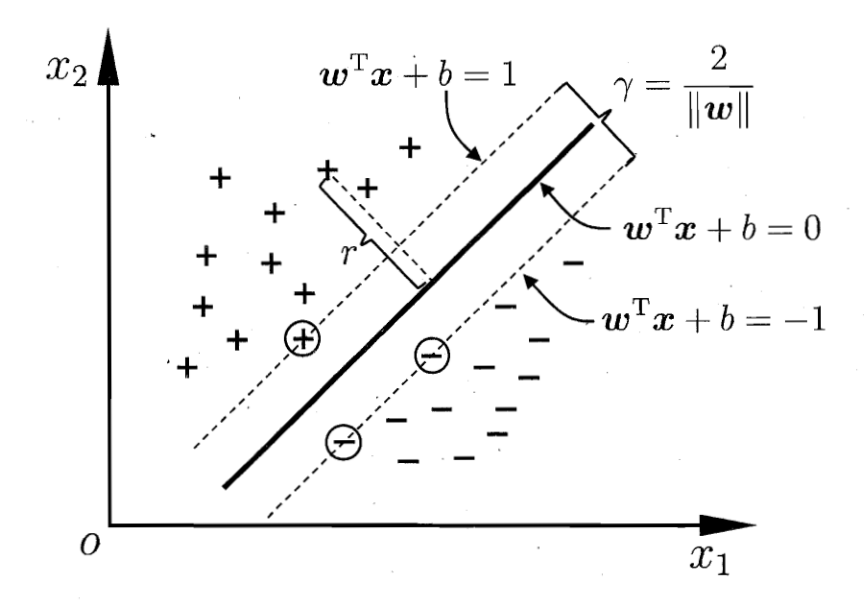
\includegraphics[width=0.4\linewidth]{fig1.png}
    \caption{支持向量与间隔}
    \label{fig:svm}
\end{figure}

其中满足 $\bm{w} ^\mathrm{T} \bm{x}+\bm{b} = \pm 1$ 的样本点,它们被称作支持向量,两个不同类的支持向量到超平面的距离之和为

\begin{equation}
  \gamma = \frac{2}{\norm{\bm{w}}}
\end{equation}

它被称为间隔。支持向量机的训练目标是最大化间隔。可以将问题表示成,
\begin{equation*}
  \begin{aligned}
  & \min _{\bm{w},b} \ \frac{1}{2} \norm{\bm{w}}^2 \\
% \end{equation*}
% \begin{equation*}
  & \mathrm{s.t.} \ y_i (\bm{w} ^\mathrm{T} \bm{x_i}+\bm{b}) \geq 1 , \quad i=1,2,\cdots,m.
    \end{aligned}
\end{equation*}

同时,上述问题可以由拉格朗日乘子法转化为对偶问题。进一步地,如果选取合适的核函数,可以将非线性问题转化为线性问题求解。

\subsection{最近邻方法}

最近邻方法,也称 KNN 算法或译K-近邻算法(k-nearest neighbors algorithm)
其实是思想特别简单的算法,即是给定测试样本,基于某种距离度量找出训练集中与其最靠近的 $k$ 个训练样本,然后基于这$k$个邻居训练样本的信息来进行预测。

通常在分类任务中可使用投票法,即选择这$k$个样本中出现最多的类标记作为预测结果;在回归任务中可使用平均法,即将这$k$个样本的实值输出标记的平均值作为预测结果,还可基于距离远近进行加权平均或者加权投票,距离越近的样本权重越大。

\subsection{随机森林}
随机森林(Random Forest)是集成学习中 Bagging 的一种。Bagging 的思想是生成基学习器之间需要有较大差异,组成的强学习器的方差减小。Bagging 多次对样本抽样产生不同的采样集。随机森林以决策树为基学习器,在训练过程中引入随机特征选择,从 $d$ 个特征中选择 $k$ 个特征,然后再从这个子集中选择一个最优特征用于划分。

随机森林简单、容易实现、可并行、计算开销小,令人惊奇的是,它在很多现实任务中展现出强大的性能。

\subsection{Boosting 类}

Boosting 是一族可将弱学习器提升为强学习器的算法。这族算法的工作机制类似:先从初始训练集训练出一个基学习器,再根据基学习器的表现,对训练样本分布进行调整,使得先前基学习器做错的训练样本在后续受到更多关注,然后基于调整后的样本分布来训练下一个基学习器;如此重复进行,直至基学习器数目达到事先指定的值$T$,最终这个$T$个基学习器进行加权结合。

Boosting 族比较出名的是 AdaBoost。从偏差-方差分解的角度看,Boosting 主要关注降低偏差。



\newpage
% -----------------------------------------------------------------------
\section{实验和结果}

\subsection{评价标准}

\begin{figure}[!h]
    \centering
    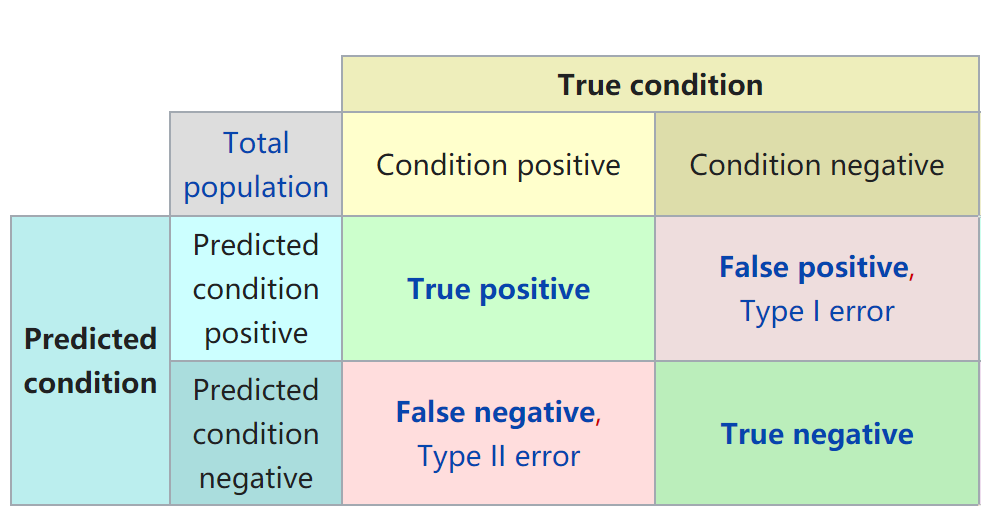
\includegraphics[width=0.7\linewidth]{fig2.png}
    \caption{二分类问题的混淆矩阵(Confusion Matrix)}
    \label{fig:conf_mat}
\end{figure}

基于混淆矩阵可以使用准确率(Precision)和召回率(Recall)来评价模型在不平衡数据上的分类精度。F-score(F1)是准确率和召回率的调和平均值。还有常用的评价指标AUCROC(Area Under Receiver-Operator Characteristic curve),需要注意的是它其实是有偏的,不适用于不平衡场景下的模型评估 \cite{davis2006relationship}。另一个指标 AUCPRC(Area Under Curve of Precision-Recall Curve)\cite{davis2006relationship}指准确率-召回率曲线下的面积。这些评价准则不会被不同类别中样本的数量所影响,因此通常被认为是“无偏的”,可以在类别不平衡的场景下使用。

由图 \ref{fig:roc2},可以看出,在ROC曲线中,由于单调,曲线越向左上角弯曲越好,而PR曲线不是单调的,那么给定对于给定 一定的recall,precision 越大越好,换言之AUCPRC越大越好。ROC曲线由于兼顾正例与负例,所以适用于评估分类器的整体性能,相比而言PR曲线完全聚焦于正例。

\begin{figure}[!h]
    \centering
    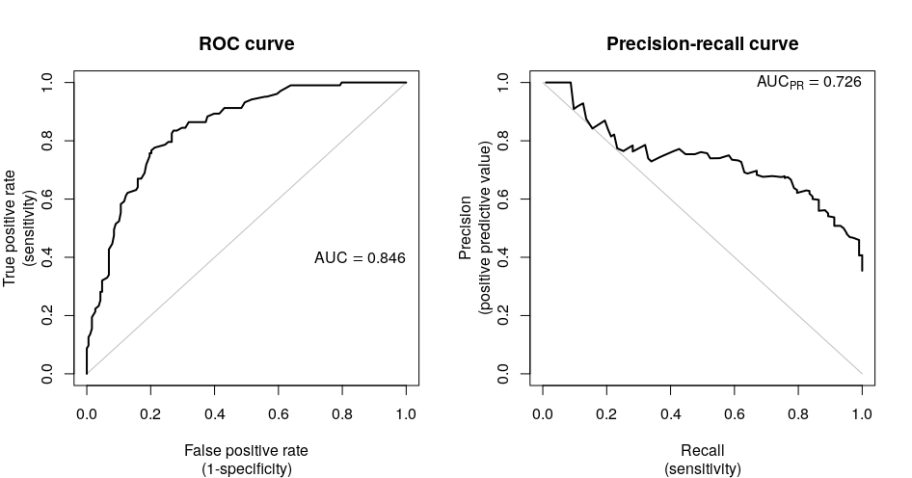
\includegraphics[width=0.8\linewidth]{roc_pr-1.png}
    \caption{ROC曲线与PR曲线}
    \label{fig:roc2}
\end{figure}

\begin{align*}
& \mathrm{Recall} = \frac{TP}{TP+FN} \qquad \mathrm{Precision} = \frac{TP}{TP+FP} \\
& \mathrm{F1-score} = 2 \cdot \frac{\mathrm{Precision}  \cdot \mathrm{Recall}}{\mathrm{Precision} + \mathrm{Recall}}
\end{align*}

% \begin{figure}[!h]
%     \centering
%     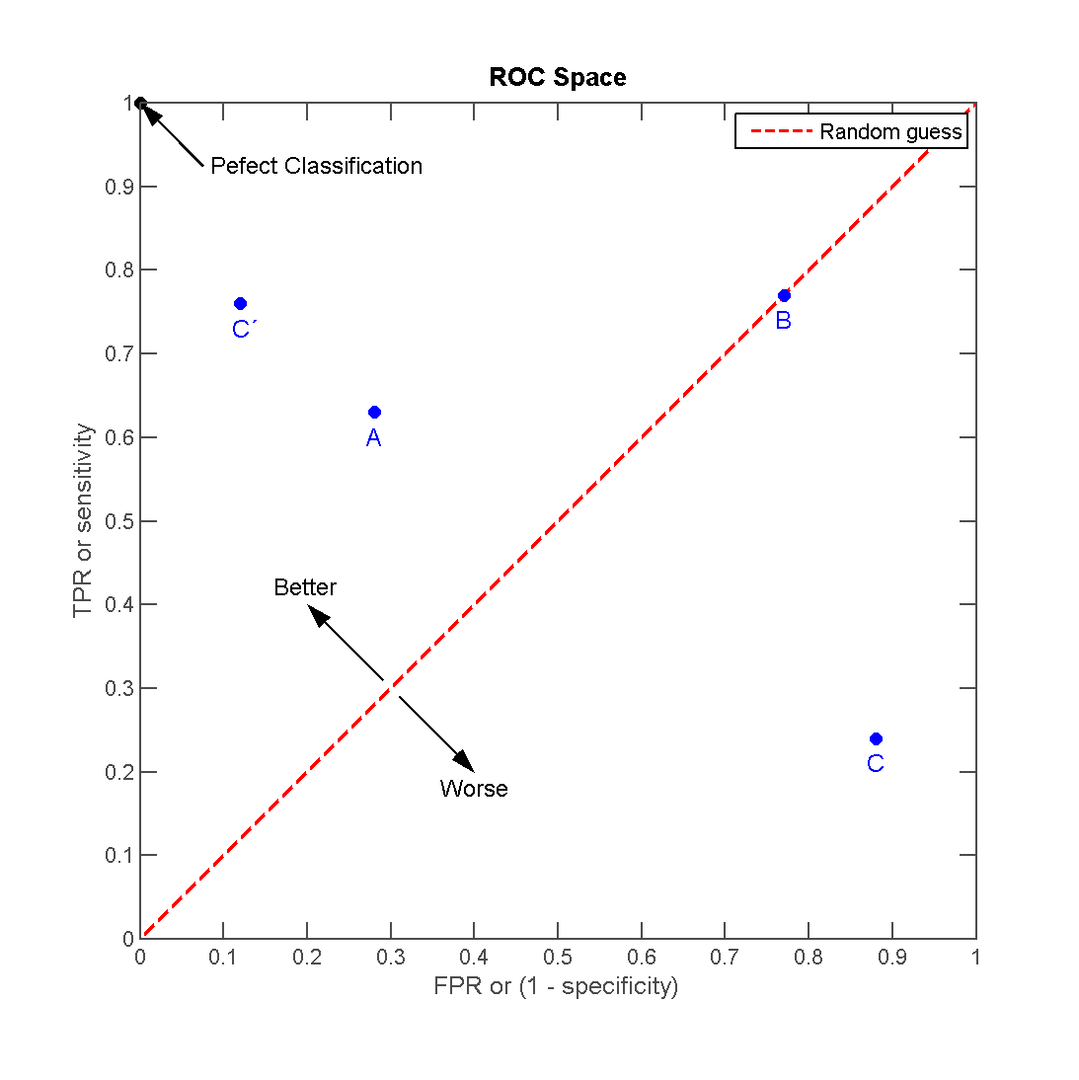
\includegraphics[width=0.6\linewidth]{1079px-ROC_space-2.png}
%     \caption{ROC曲线}
%     \label{fig:roc}
% \end{figure}


% https://zhuanlan.zhihu.com/p/66373943
% https://medium.com/nlp-tsupei/roc-pr-%E6%9B%B2%E7%B7%9A-f3faa2231b8c

\subsection{训练与测试}
根据已有数据:训练集8285个样本,其中7819个负类,466个正类;测试集2071个样本,其中1955个负类,117个正类。训练时,将训练集的8285个样本随机按照3:1的比例分成训练集 (train set) 和验证集 (validation set)。测试集(test set)的2071个样本,仅用于训练结束后的性能测试,不参与模型训练。

\subsection{实验结果}

% ============================================================================
\subsubsection{逻辑回归}
逻辑回归采用 \texttt{sklearn.linear\_model} 中的 \texttt{LogisticRegression} 训练,分四分之一的训练集 (train set) 数据作为验证集 (validation set),使用 \texttt{GridSearchCV} 搜索最优参数:

\begin{itemize}
    \item \texttt{C}:正则化系数$\lambda$的倒数,\texttt{float}类型,默认为1.0。越小的数值表示越强的正则化。搜索范围:$[0.001, 0.01, 0.1, 1, 10, 100, 1000]$。
    \item \texttt{penalty}:惩罚项,\texttt{str}类型,可选参数为``l1"和``l2",默认为``l2"。搜索范围:``l1"和``l2"。
\end{itemize}

\noindent 其他不需要搜索的参数设置:
\begin{itemize}
    \item \texttt{class\_weight}:用于标示分类模型中各种类型的权重,可以是一个字典或者``balanced"字符串,默认为不输入,也就是不考虑权重,即为None。如果选择输入的话,可以选择 balanced 让类库自己计算类型权重,或者自己输入各个类型的权重。如果\texttt{class\_weight}选择 balanced,那么类库会根据训练样本量来计算权重。某种类型样本量越多,则权重越低,样本量越少,则权重越高。当\texttt{class\_weight}为 balanced 时,类权重计算方法如下:\texttt{n\_samples / (n\_classes * np.bincount(y))}。\texttt{n\_samples} 为样本数,\texttt{n\_classes} 为类别数量,\texttt{np.bincount(y)} 会输出每个类的样本数。
    
    \item \texttt{solver}:优化算法选择参数,只有五个可选参数,即newton-cg, lbfgs, liblinear, sag, saga。默认为 liblinear。\texttt{solver} 参数决定了对逻辑回归损失函数的优化方法。对于本数据集,较小数据集的二元分类 liblinear 即可。
    
    \item \texttt{n\_jobs}:并行数,或者可视作内核数。\texttt{int}类型,默认为1。为1时,用CPU的一个内核运行程序;为2时,用CPU的2个内核运行程序。为-1的时候,用所有CPU的内核运行程序。
\end{itemize}

\noindent 使用 \texttt{GridSearchCV} 搜索 \texttt{C} 和 \texttt{penalty}。搜索过程采用5-Fold,评价标准采用 \texttt{sklearn} 中定义的 `f1\_macro',marco 意为每一类求F1(准确率和召回率的调和平均),然后直接取无权平均(各类别F1的权重相同)。 

搜索结果:\texttt{C} 取 0.01, \texttt{penalty} 取 `l1'。图 \ref{fig:result:lg} 是最优参数在测试集 (test set) 中的混淆矩阵。表 \ref{tb:lg} 为对应的评价数值。

% \begin{minipage}{\linewidth}
\begin{table}[!h]
    \centering
    \renewcommand{\arraystretch}{1.5}
    % \begin{minipage}{.49\linewidth}
    \begin{tabular}{|r|c|c|c|}
        \hline
                  & Precision & Recall & F1-score \\ \hline
        -1        &     0.97051     &     0.77442   &    0.86145      \\ \hline
        1         &     0.13867      &     0.60684   &   0.22576       \\ \hline
        macro avg &      0.55459     &     0.69063   &    0.54360      \\ \hline
    \end{tabular}
    \caption{逻辑回归的评价}
    \label{tb:lg}
    % \end{minipage}
\end{table}
% \hfill
\begin{figure}[!h]
    \centering
    % \begin{minipage}{.49\linewidth}
    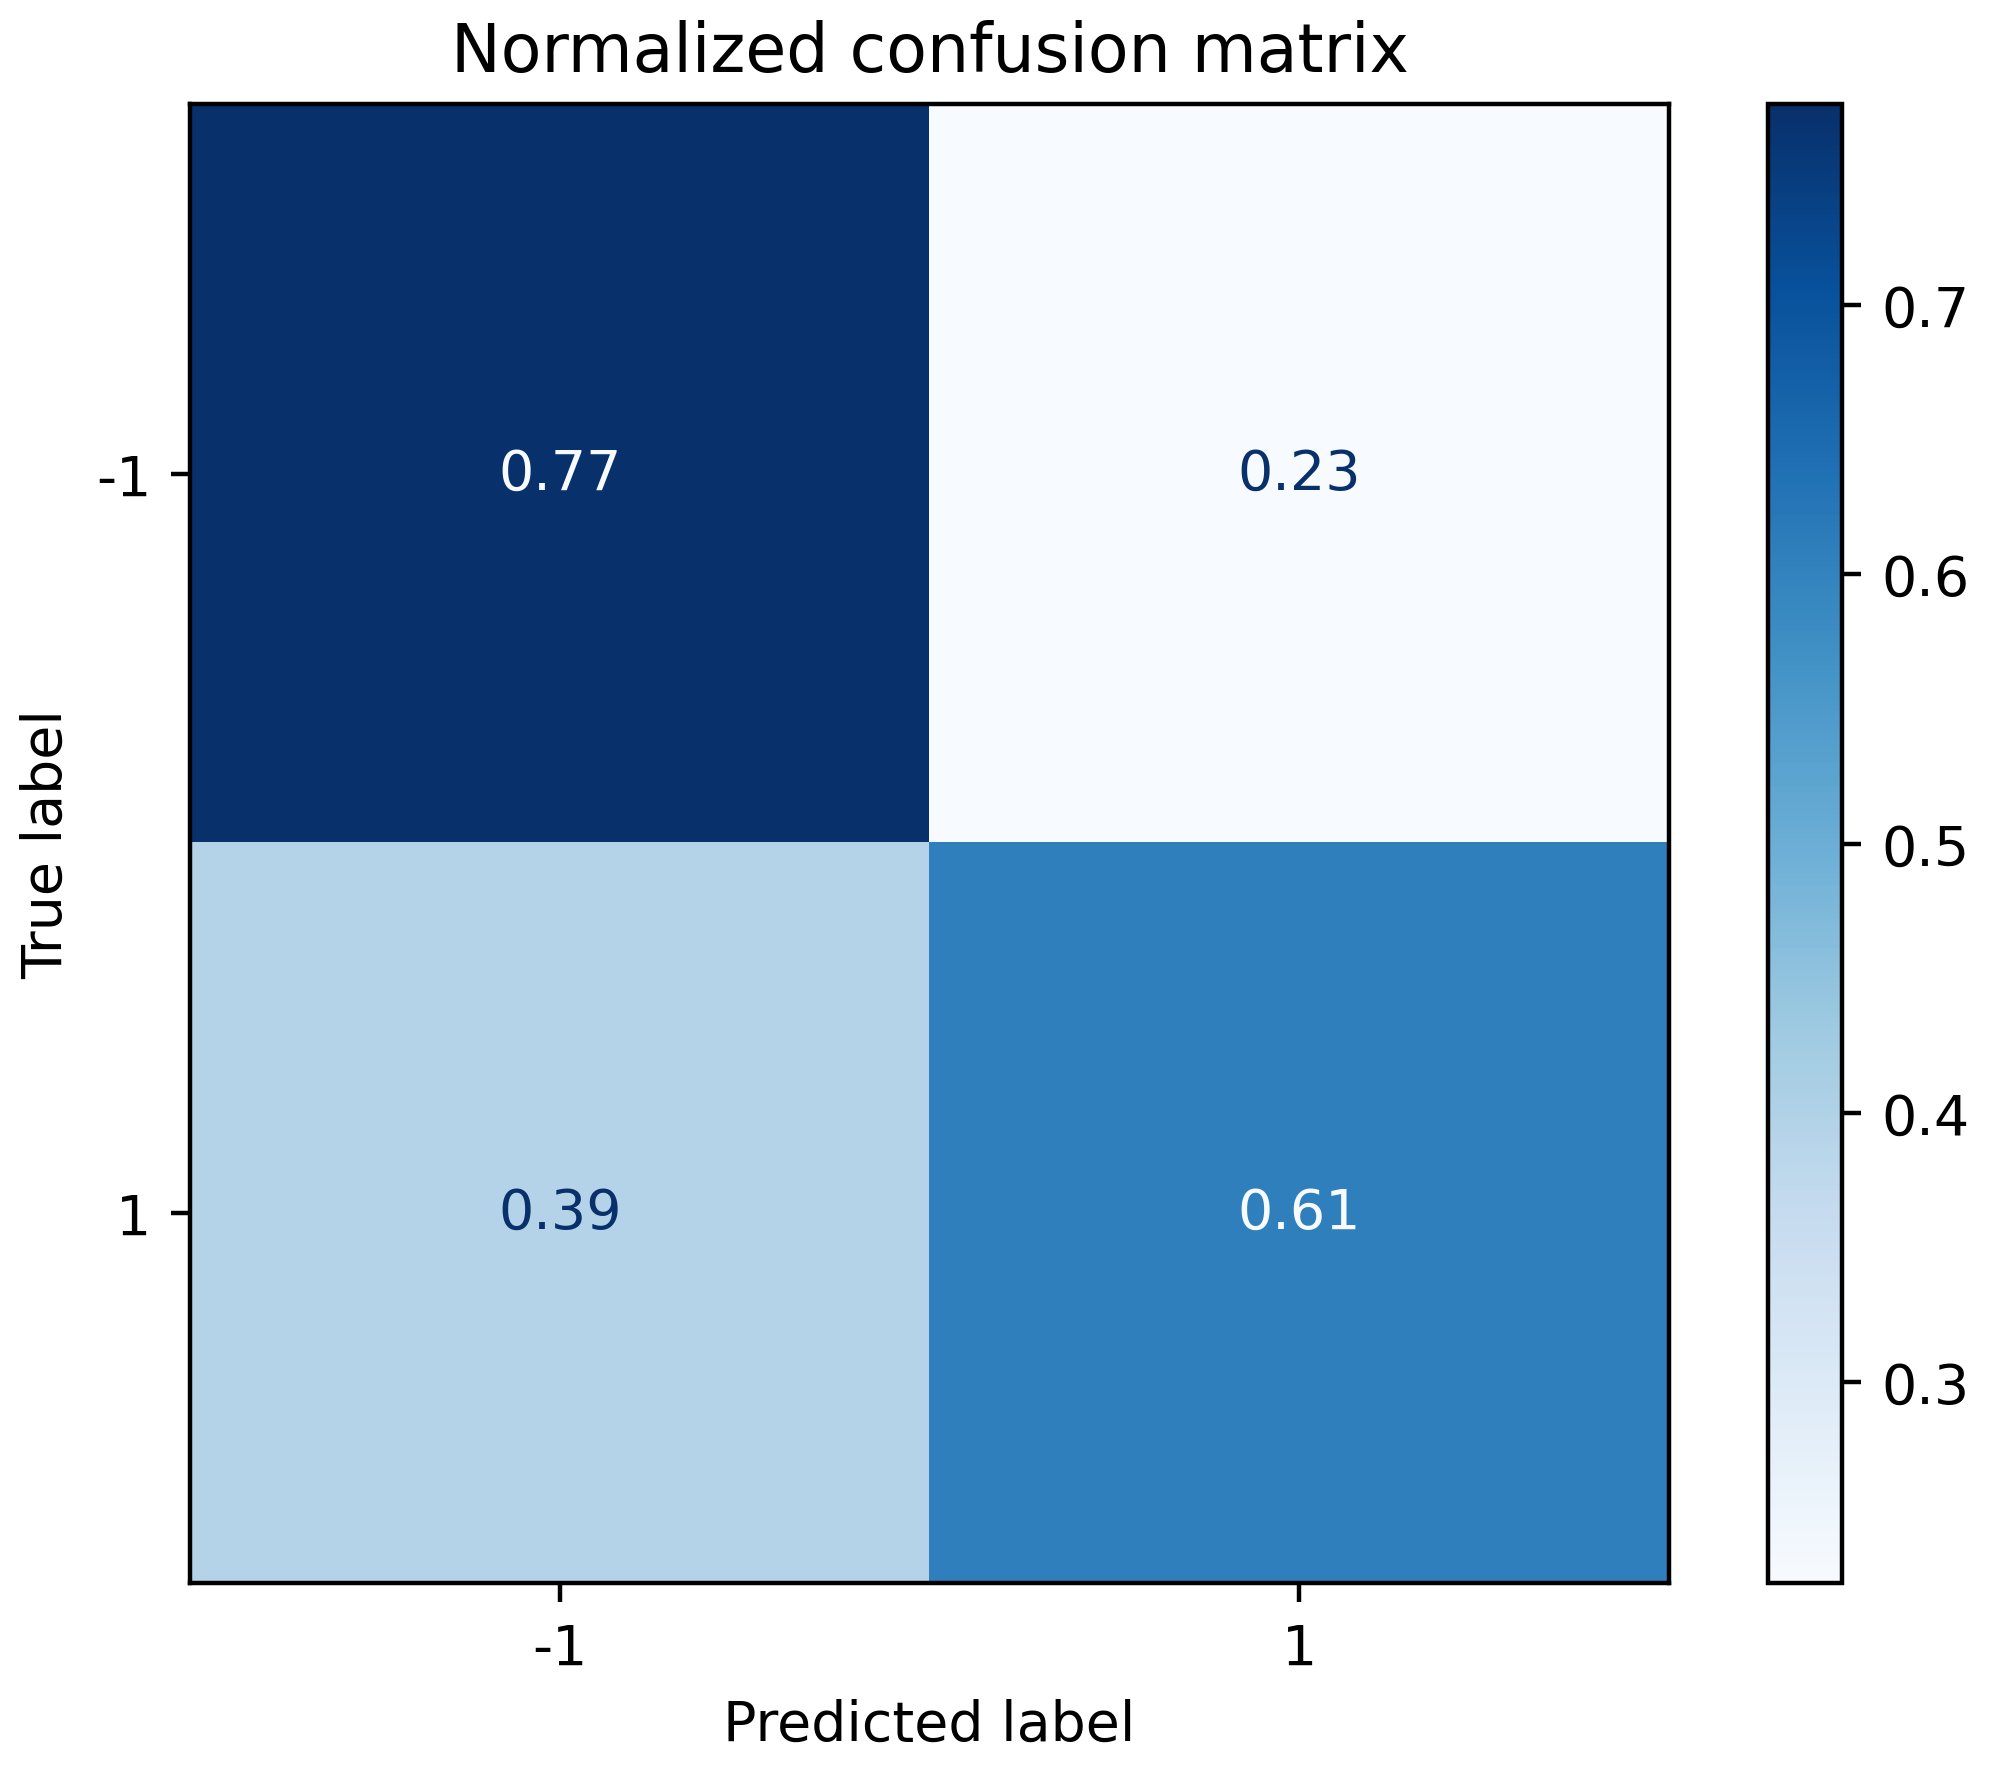
\includegraphics[width=0.48\linewidth]{LR_confus_mat-norm.png}
    \caption{逻辑回归的混淆矩阵(测试集)}
    \label{fig:result:lg}
    % \end{minipage}
\end{figure}
% \end{minipage}

% ============================================================================
\subsubsection{支持向量机(SVM)}

\texttt{sklearn} 中可以选择线性SVM,也可以采用RBF (径向基函数核)为核函数,转化为非线性问题求解。本实验对2种SVM都进行了训练,选择最优参数。从图 \ref{fig:result:svm} 看出,虽然线性SVM在少数类上召回率没有使用RBF的核SVM好,但是线性SVM在F1-score上的表现更好。

\begin{table}[!h]
\renewcommand{\arraystretch}{1.5}
\parbox{.45\linewidth}{
\centering
    \begin{tabular}{|r|c|c|c|}
        \hline
                  & Precision & Recall & F1-score \\ \hline
        -1        &     0.96357     &     0.86598   &    0.91218      \\ \hline
        1         &     0.16825      &     0.45299   &   0.24537       \\ \hline
        macro avg &      0.56591     &     0.65949   &    0.57877      \\ \hline
    \end{tabular}
    \caption{线性SVM的评价}
}
\hfill
\parbox{.45\linewidth}{
\centering
    \begin{tabular}{|r|c|c|c|}
        \hline
                  & Precision & Recall & F1-score \\ \hline
        -1        &     0.97051     &     0.75754   &    0.85090      \\ \hline
        1         &     0.13187      &     0.61538   &   0.21719       \\ \hline
        macro avg &      0.55119     &     0.68646   &    0.53405      \\ \hline
    \end{tabular}
    \caption{RBF核SVM的评价}
}
\end{table}


\begin{figure}[!h]
    \centering
    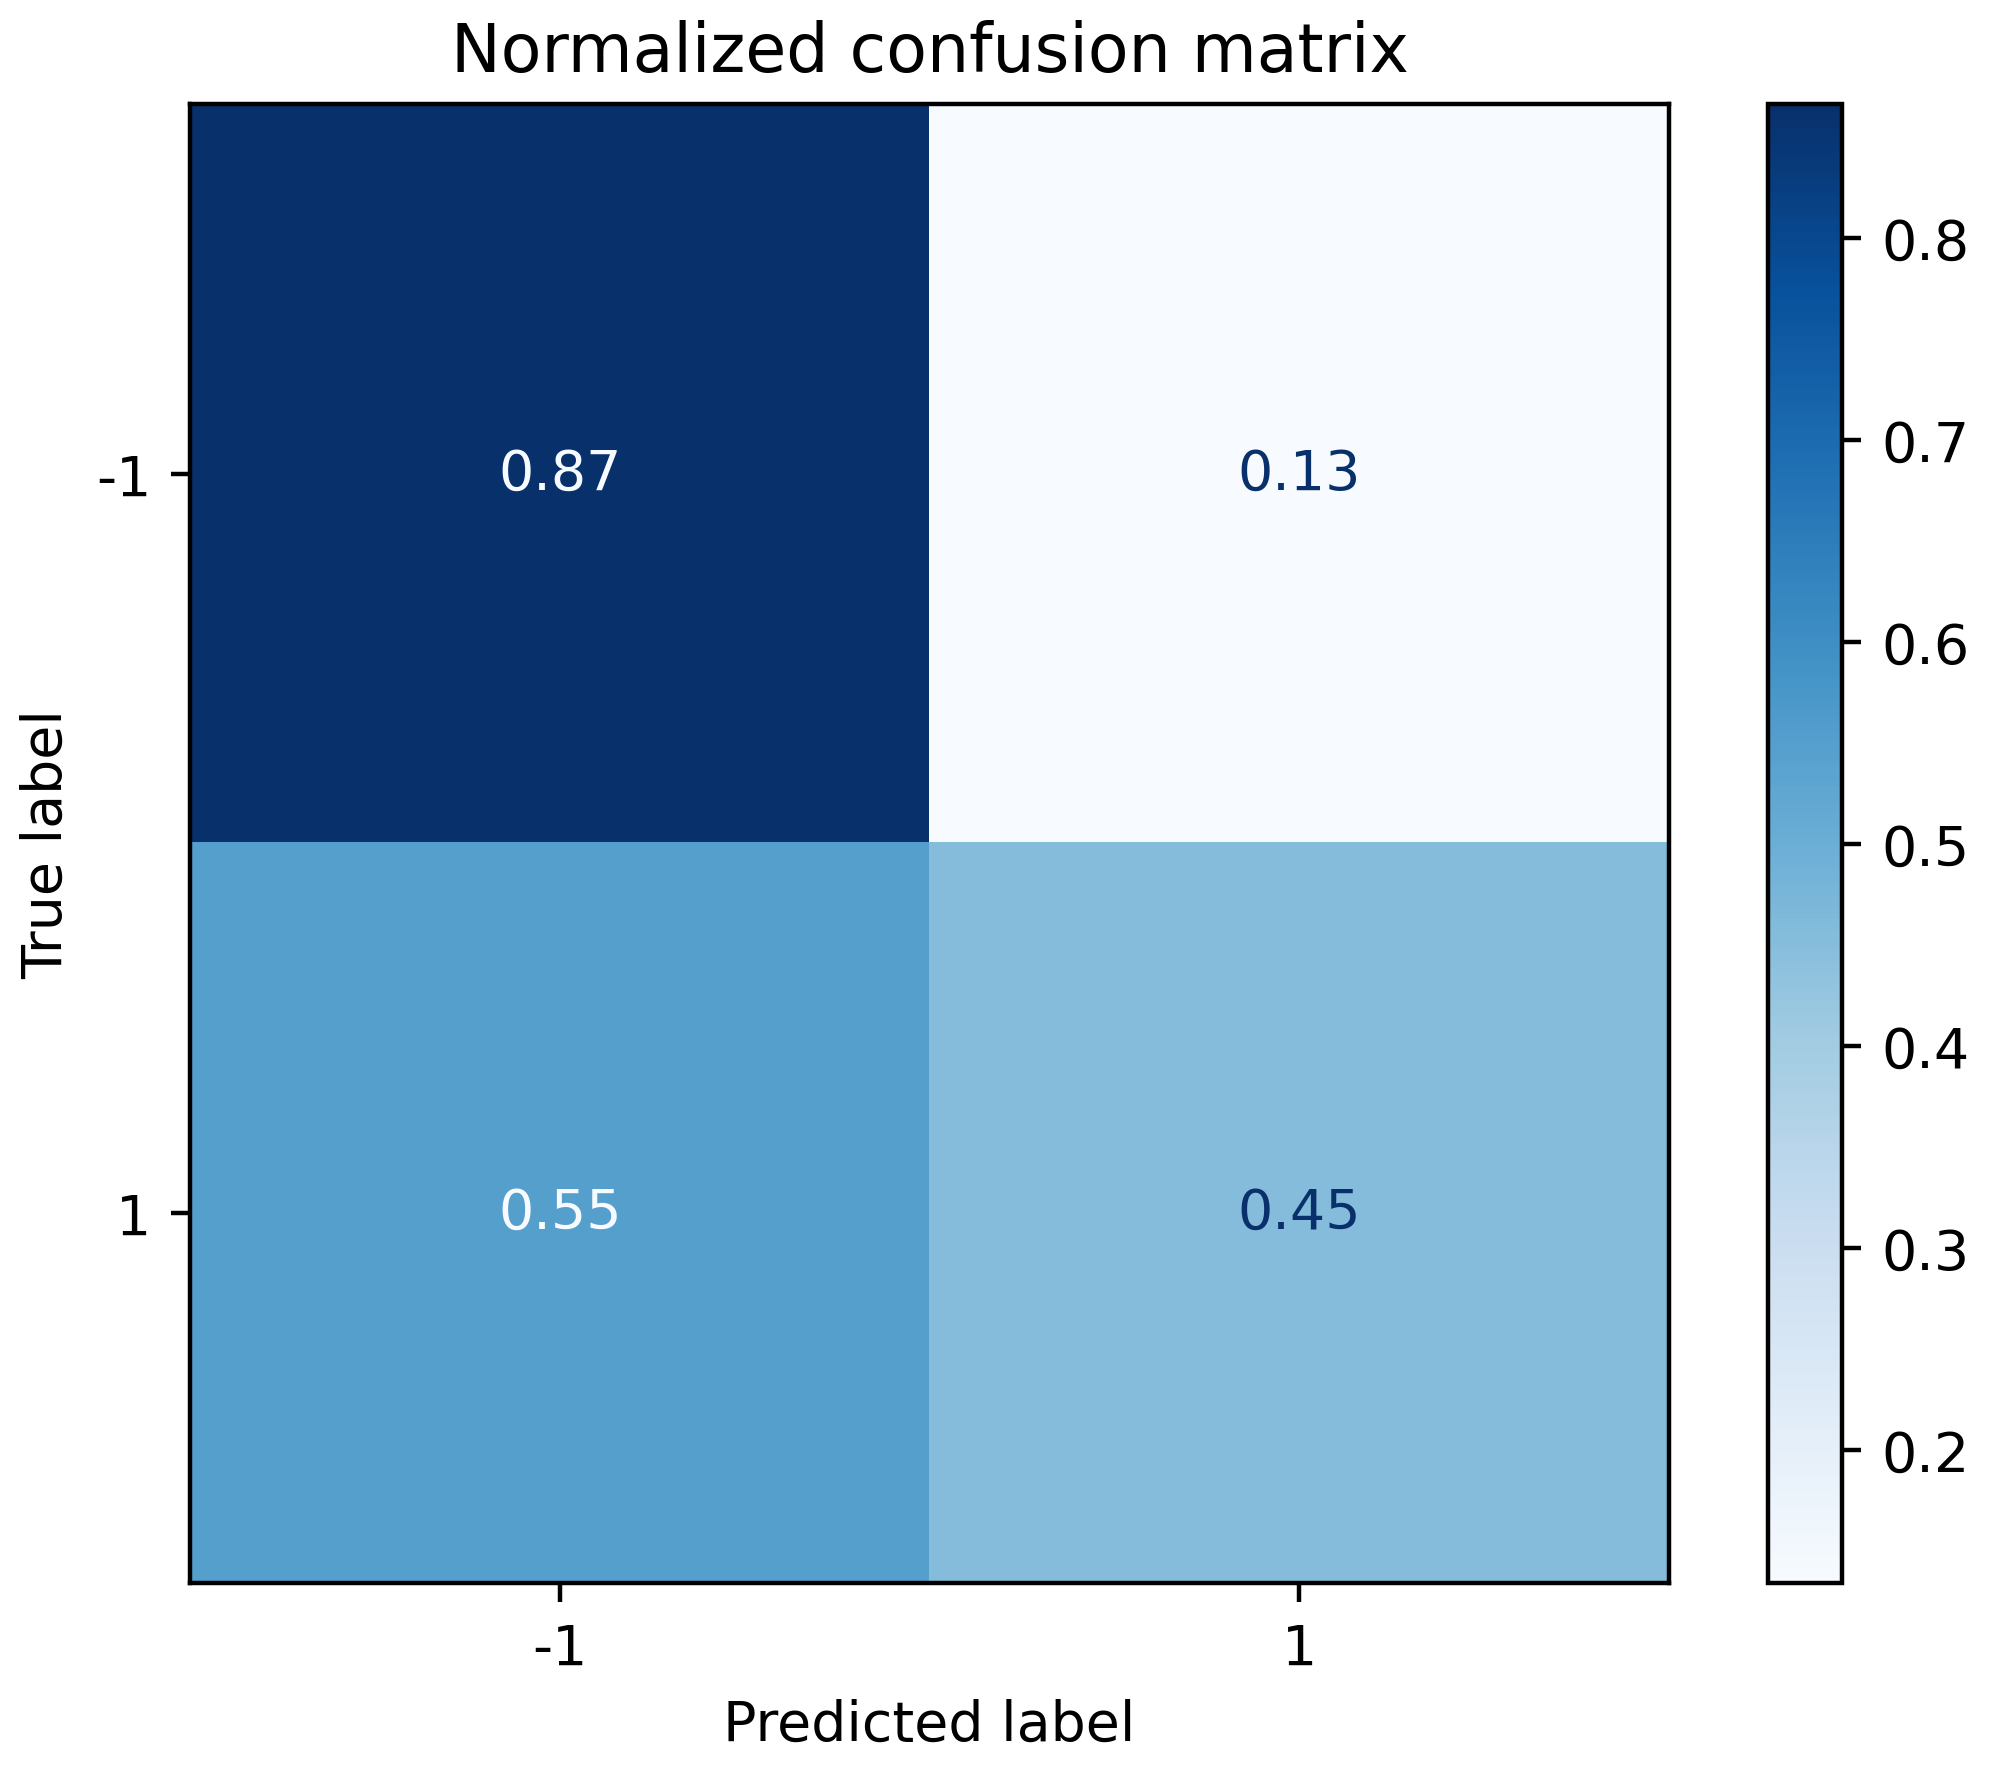
\includegraphics[width=0.48\linewidth]{LinearSVC_confus_mat-norm.png}
    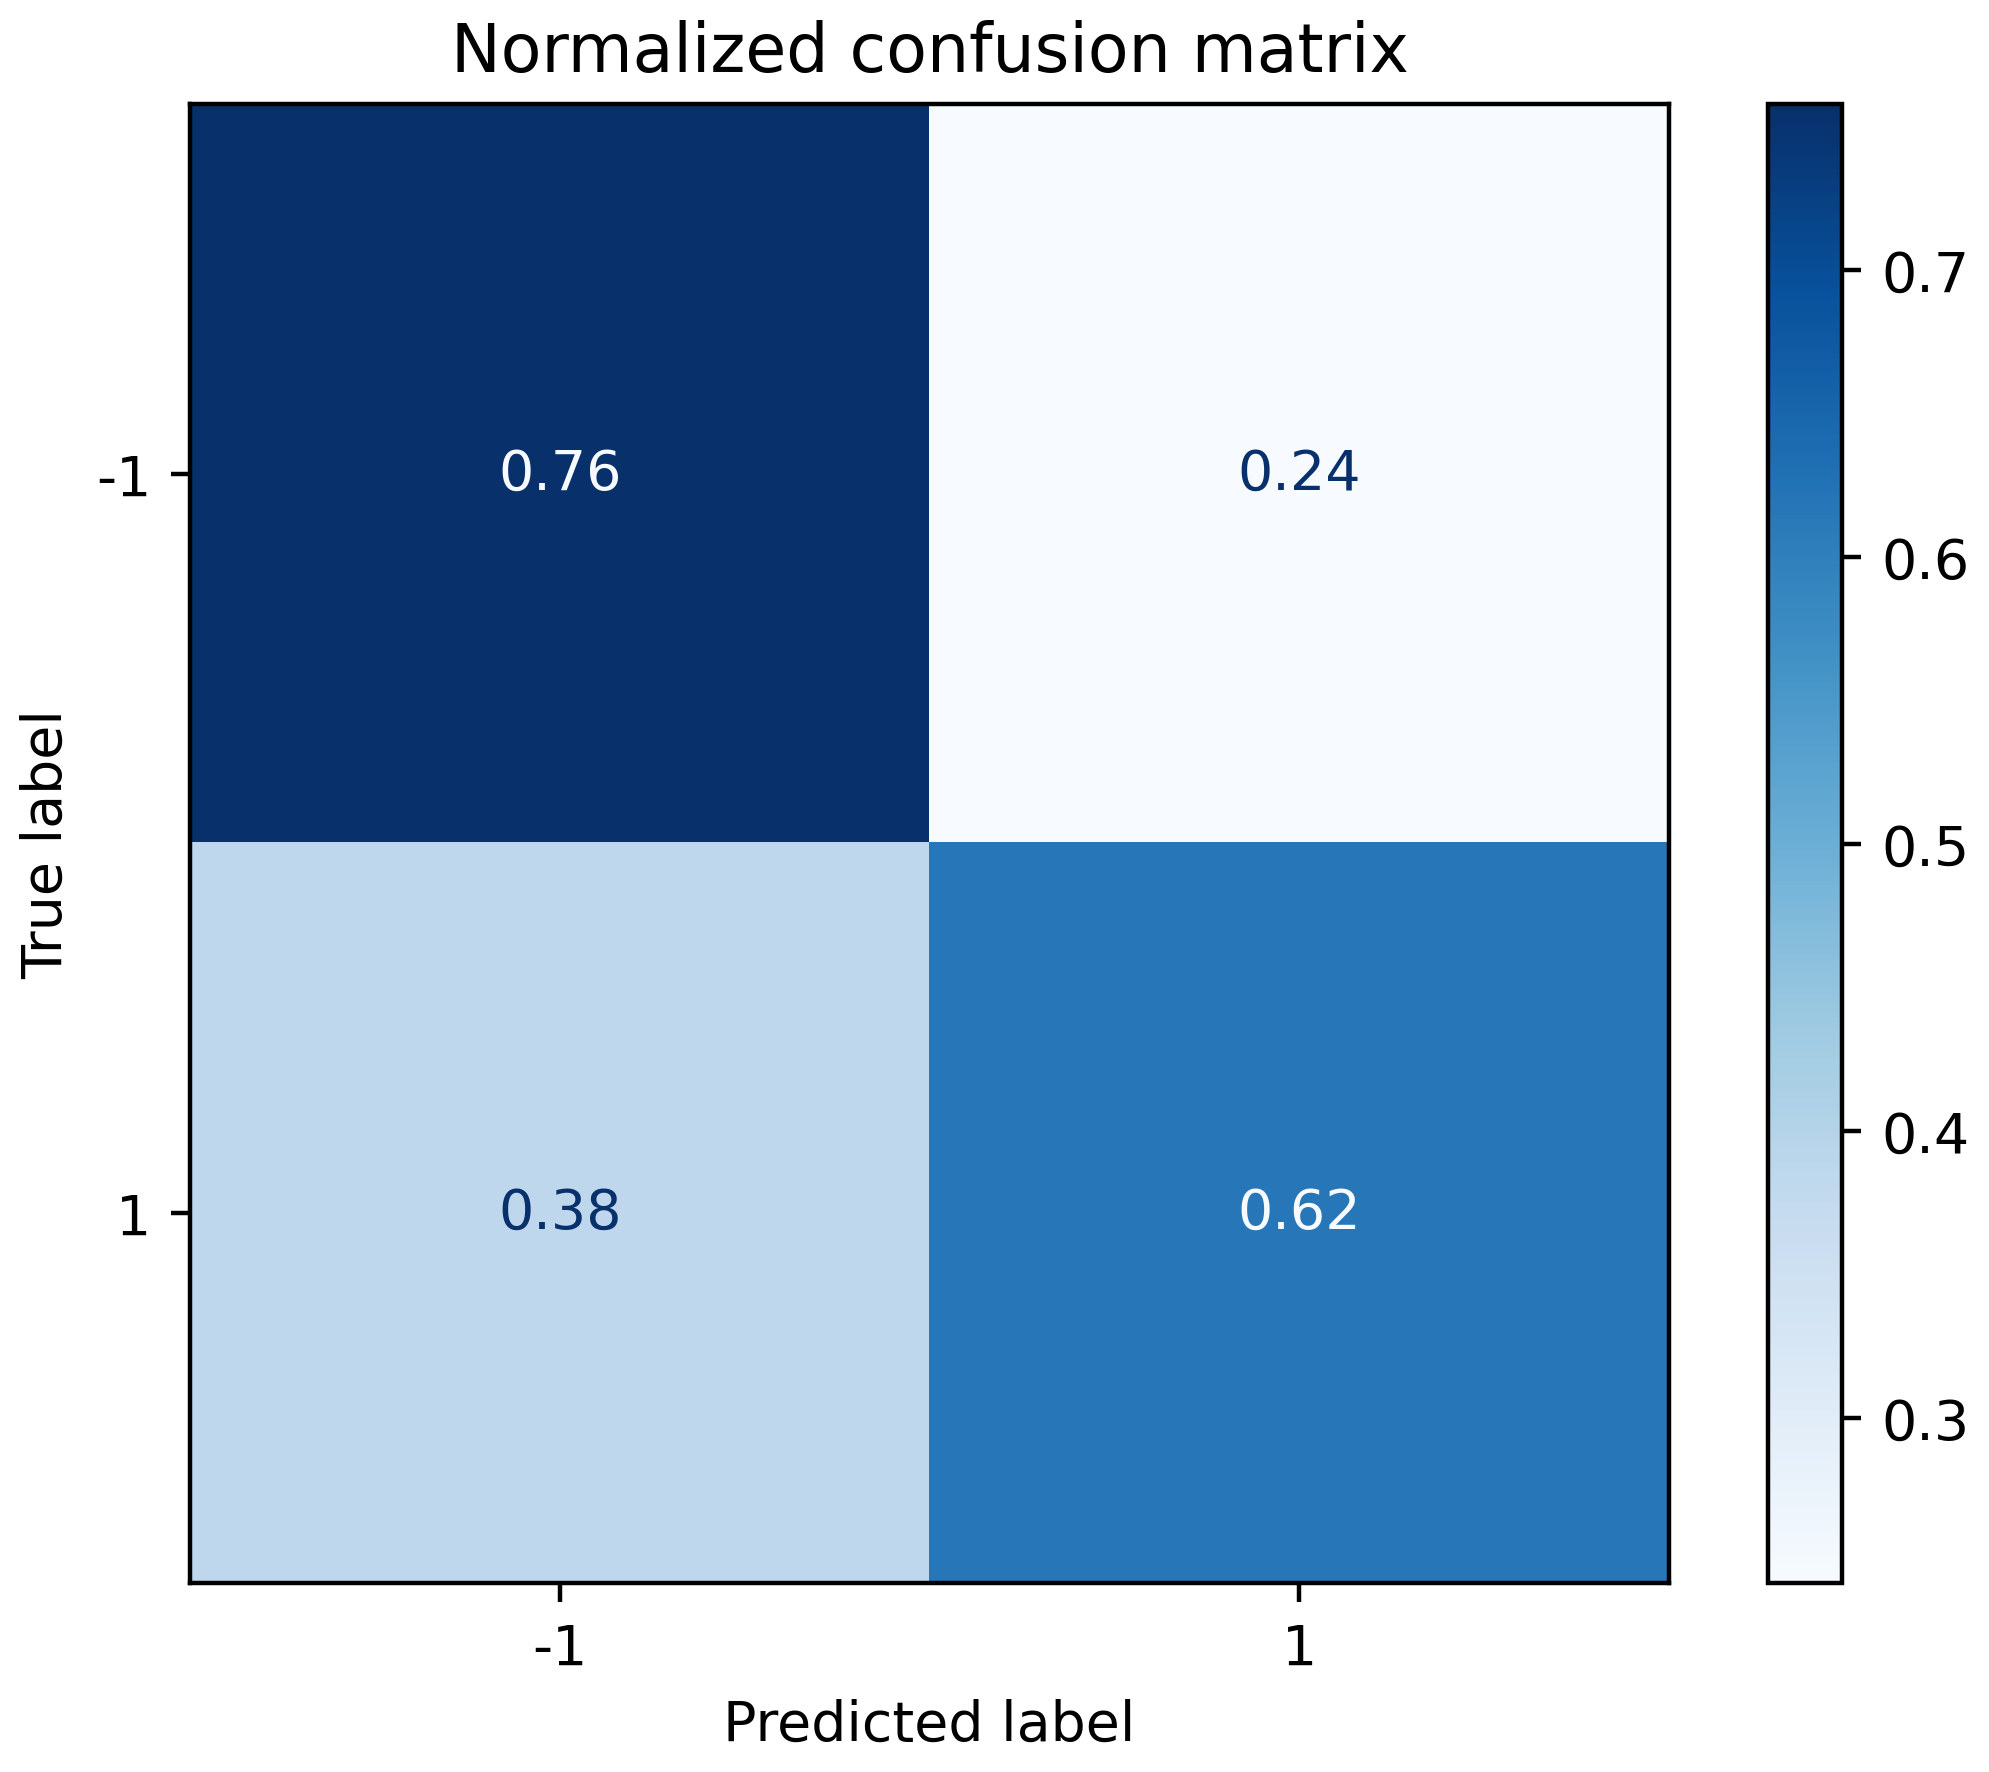
\includegraphics[width=0.48\linewidth]{svm_confus_mat-norm.png}
    \caption{线性SVM,RBF核SVM的混淆矩阵(测试集)}
    \label{fig:result:svm}
\end{figure}

在模型调参上,和逻辑回归类似使用 \texttt{GridSearchCV} 搜索 \texttt{C},\texttt{kernel},\texttt{gamma},\texttt{penalty},等常见参数。

搜索结果:
\begin{itemize}
    \item 线性SVM \texttt{C} 取 10, \texttt{penalty} 取 `l2';
    \item 非线性SVM \texttt{C} 取 0.01, \texttt{kernel} 取 `rbf',\texttt{gamma} 取 `auto'。

\end{itemize}

% ============================================================================
\subsubsection{最近邻方法}
% \todo{没有参数\texttt{class\_weight}}

最近邻方法的表现非常依赖于样本之间的距离这一概念的定义,常见定义是欧式距离$\sqrt{\sum_{i=1}^{n}{(x_{i}-y_{i})^{2}}}$,曼哈顿距离$\sqrt{\sum_{i=1}^{n}{|x_{i}-y_{i}|}}$;另一个会影响模型表现的是选择邻居的个数,以及对应的权重。
这里同样使用 \texttt{GridSearchCV} 搜索其会影响表现的参数:
\begin{itemize}
    \item \texttt{n\_neighbors}:选取几个最近的邻居,默认是5,搜索范围放宽到$[3, 5, 7, 9]$,
    \item \texttt{weights}:邻居的权重是否考虑距离,可以选`uniform' 不考虑,或者`distance'根据距离决定权重,
    \item \texttt{p},Minkowski metric的指数参数。当$p=1$时,与曼哈顿距离等价,当$p=2$时与欧氏距离等价。
\end{itemize}

根据搜索结果:\texttt{n\_neighbors}: 3, \texttt{p}: 1, \texttt{weights}: 'distance',得到以下图\ref{fig:result:knn}和表\ref{tb:knn}。

\begin{table}[!h]
    \centering
    \renewcommand{\arraystretch}{1.5}
    \begin{tabular}{|r|c|c|c|}
        \hline
                  & Precision & Recall & F1-score \\ \hline
        -1        &     0.94403     &     0.97494   &    0.95924      \\ \hline
        1         &     0.07547      &     0.03419   &   0.04706       \\ \hline
        macro avg &      0.50975     &     0.50456   &    0.50315      \\ \hline
    \end{tabular}
    \caption{KNN的评价}
    \label{tb:knn}
\end{table}

\begin{figure}[!h]
    \centering
    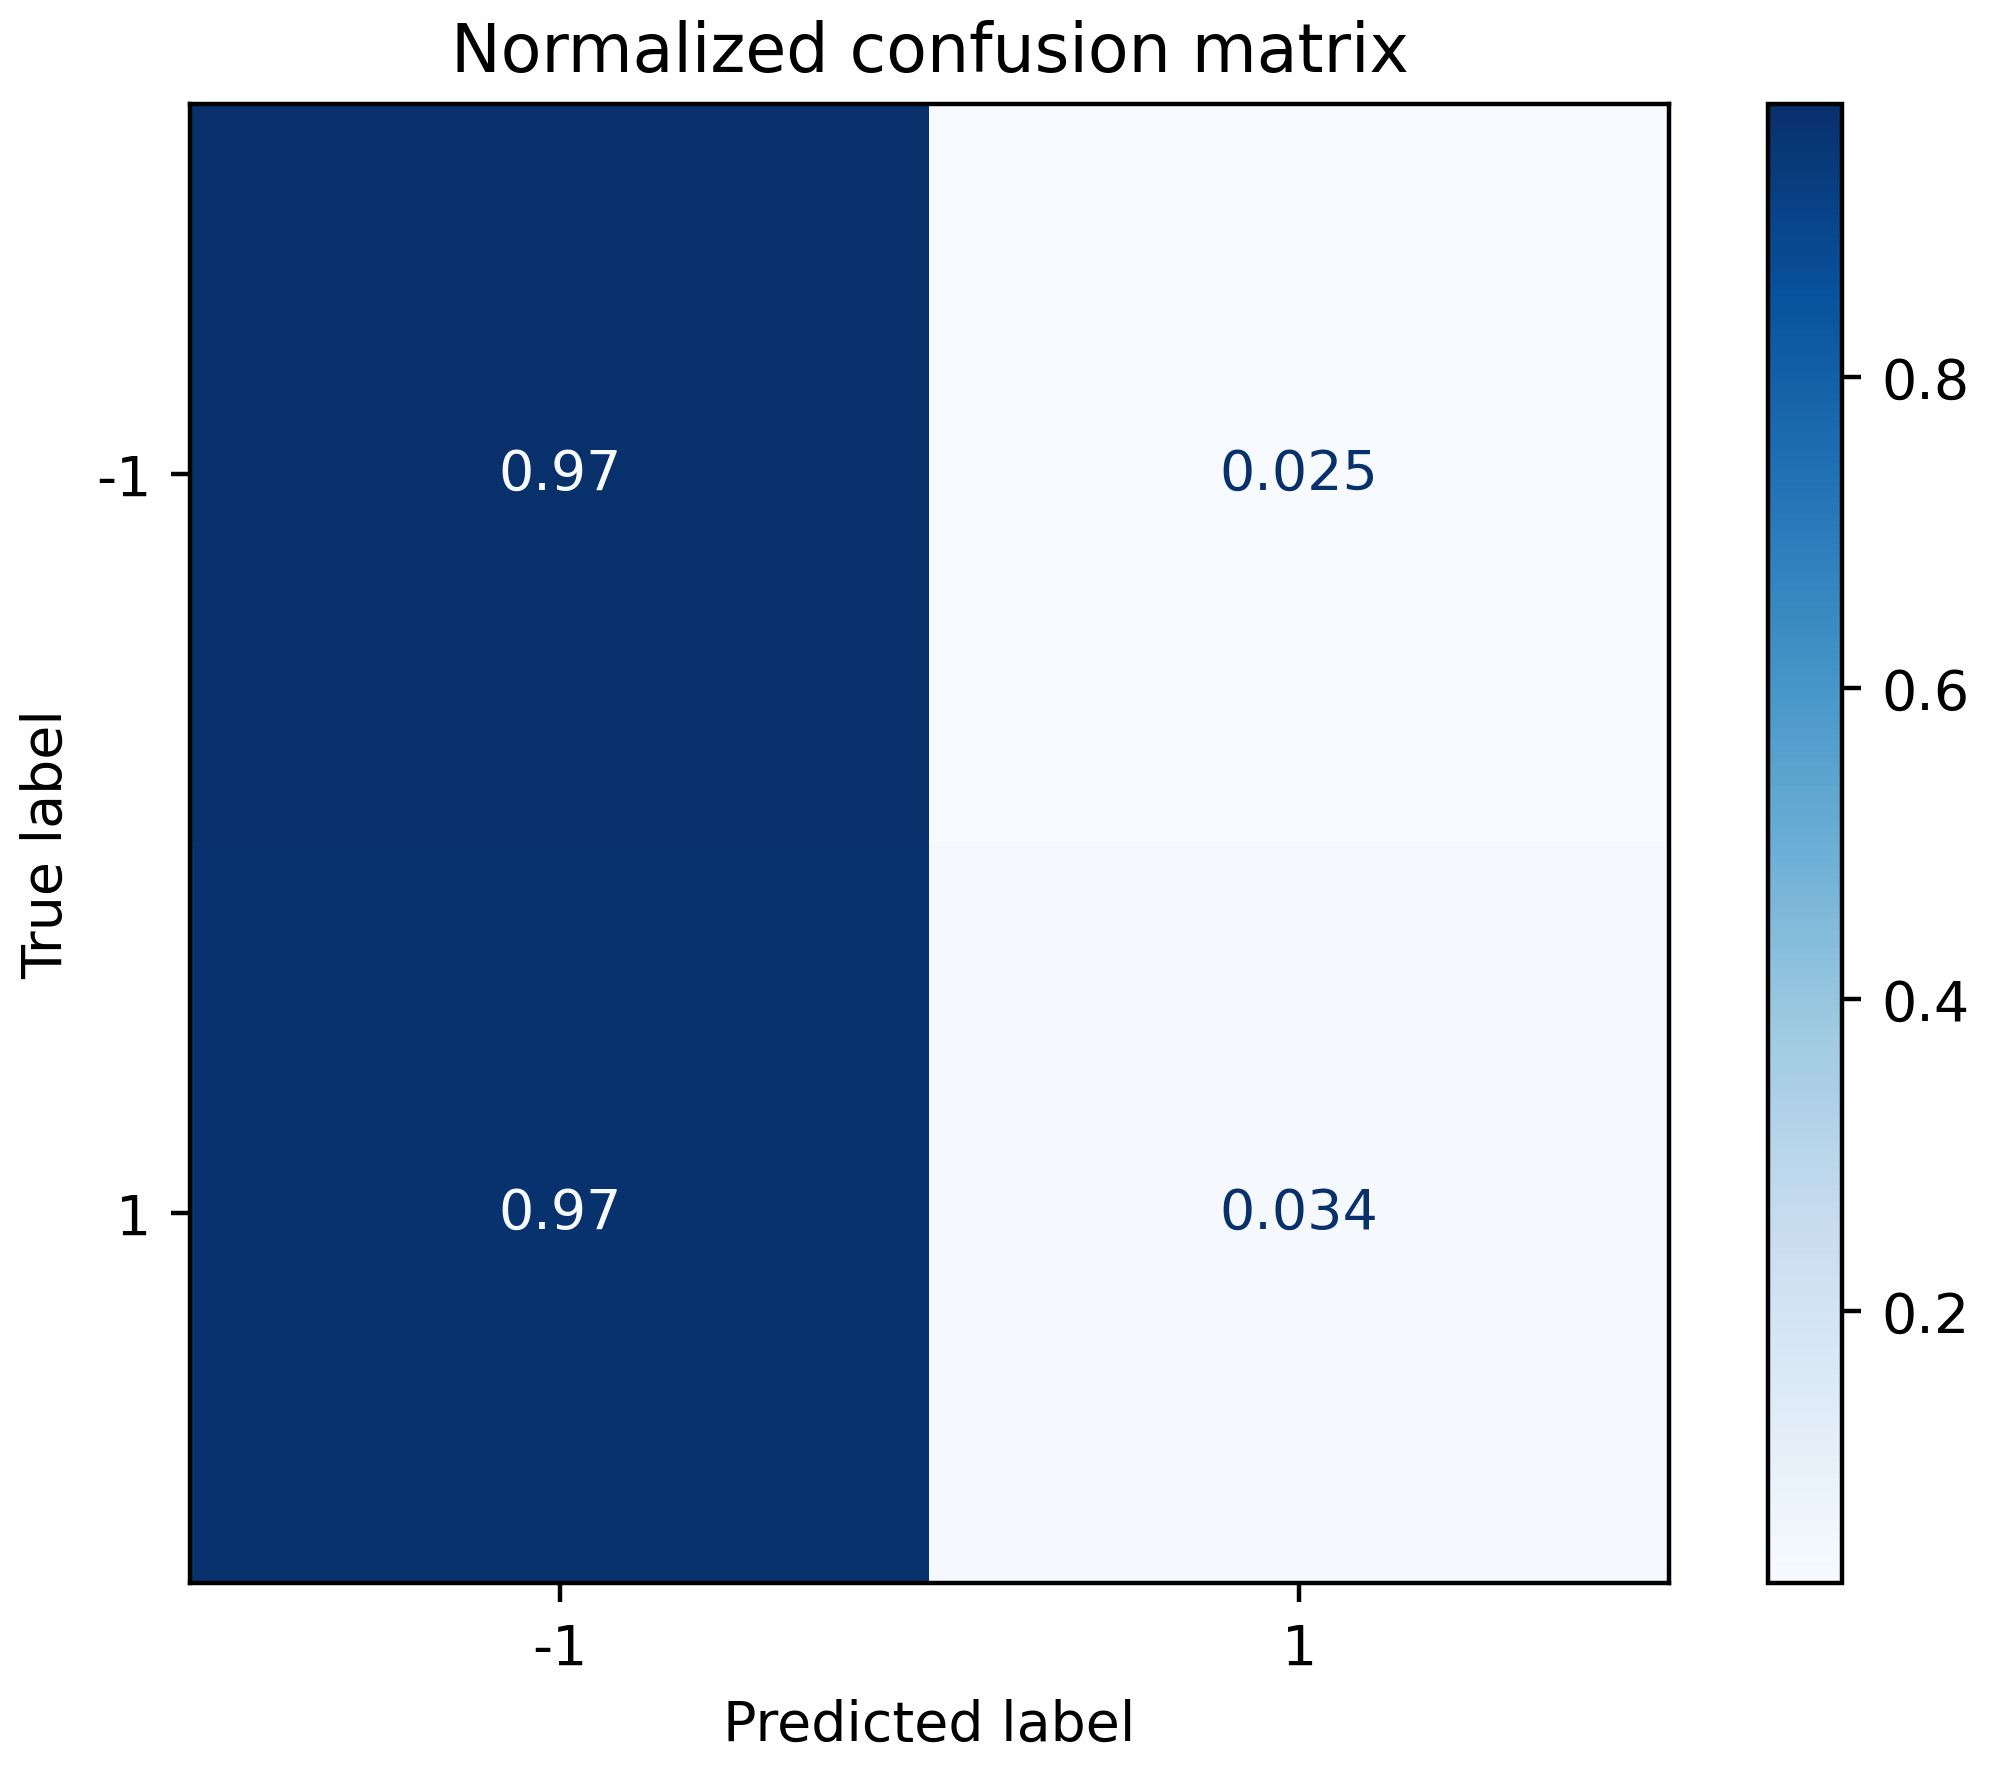
\includegraphics[width=0.48\linewidth]{KNN_confus_mat-norm.png}
    \caption{KNN的混淆矩阵(测试集)}
    \label{fig:result:knn}
\end{figure}

% ============================================================================
\subsubsection{随机森林}
随机森林是典型的集成学习的实现,期望由多个弱学习器集成得到一个表现优秀的强学习器。所以随机森林常见的参数有如下:
\begin{itemize}
    \item \texttt{n\_estimators}:弱学习器的个数。一般来说 \texttt{n\_estimators}太小,容易欠拟合,\texttt{n\_estimators} 太大,计算量会太大,并且 \texttt{n\_estimators} 到一定的数量后,再增大 \texttt{n\_estimators} 获得的模型提升会很小,所以一般选择一个适中的数值。默认是100;
    \item \texttt{max\_depth}: 默认为None,如果采用默认值,决策树在建立子树的时候不会限制子树的深度,限制深度可以防止过拟合;
    \item \texttt{bootstrap}:是否有放回的采样。
\end{itemize}

在实验中发现,限制深度 \texttt{max\_depth} 会使得多数类表现下降,但是少数类表现提升明显。
根据搜索结果:\texttt{n\_estimators}: 170, \texttt{max\_depth}: 7, \texttt{bootstrap}: True,得到以下图\ref{fig:result:rfc}和表\ref{tb:rfc}。

\begin{table}[!h]
    \centering
    \renewcommand{\arraystretch}{1.5}
    \begin{tabular}{|r|c|c|c|}
        \hline
                  & Precision & Recall & F1-score \\ \hline
        -1        &     0.97303     &     0.75652   &    0.85122      \\ \hline
        1         &     0.13768      &     0.64957   &   0.22720       \\ \hline
        macro avg &      0.55535     &     0.70305   &    0.53921      \\ \hline
    \end{tabular}
    \caption{随机森林的评价}
    \label{tb:rfc}
\end{table}

\begin{figure}[!h]
    \centering
    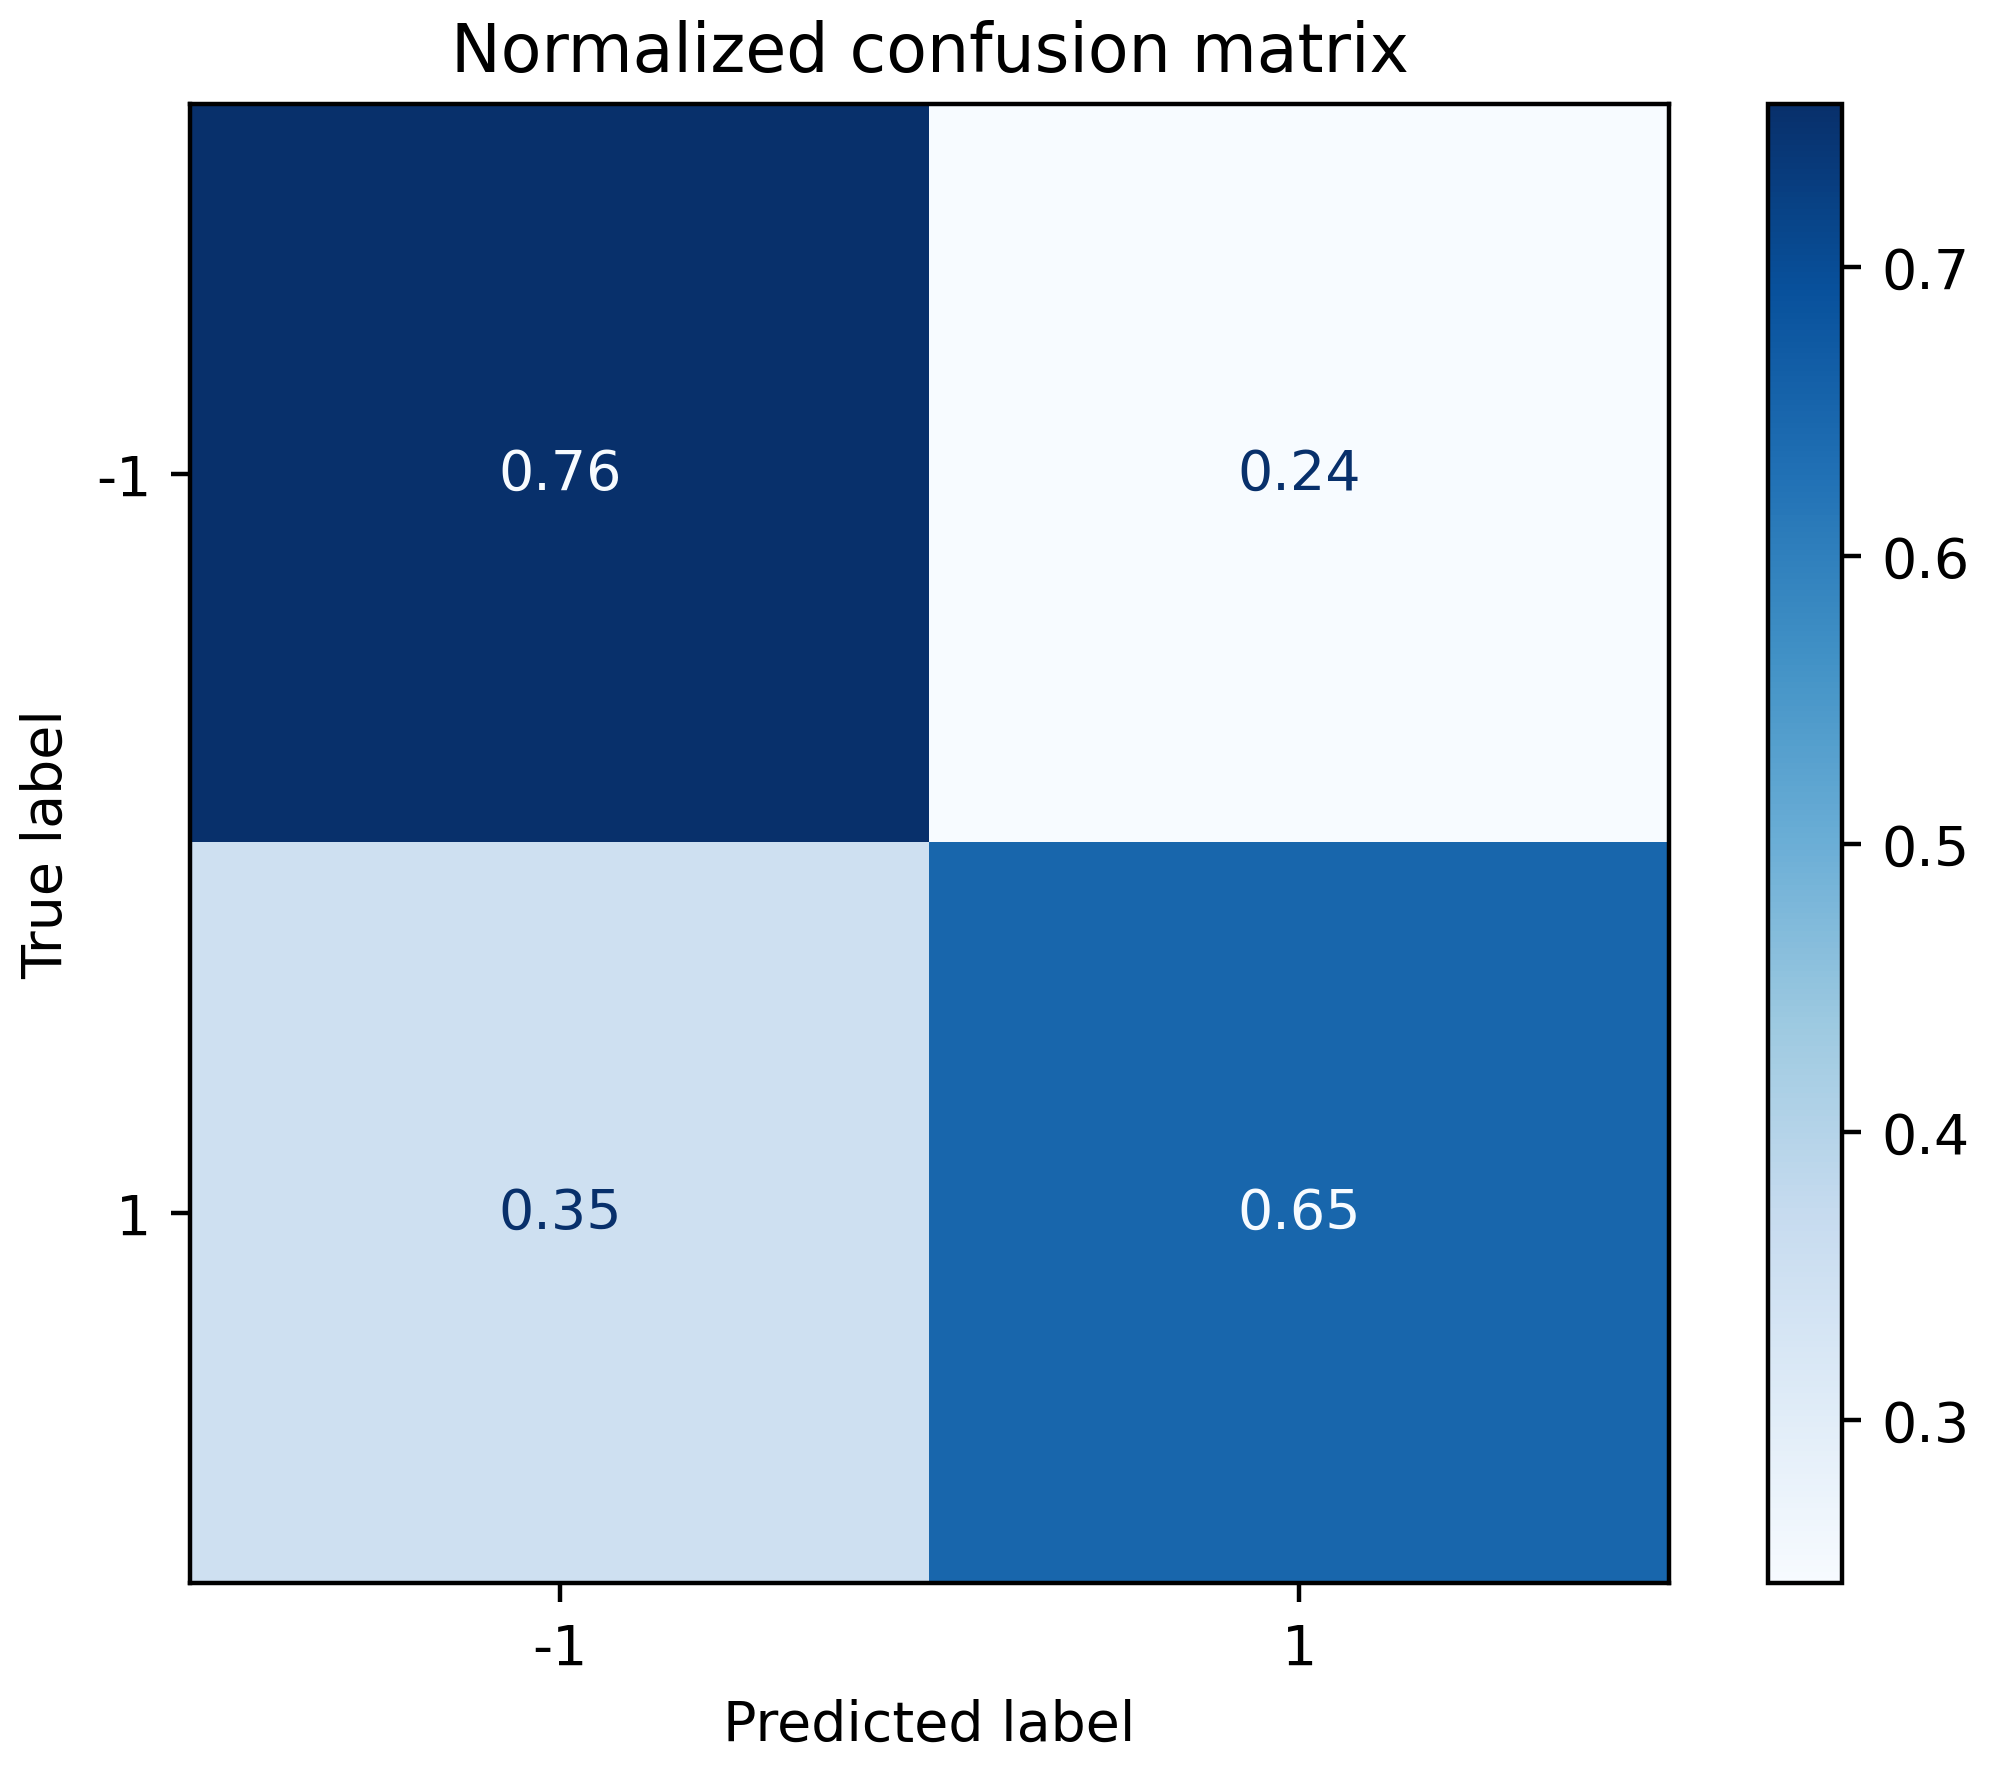
\includegraphics[width=0.48\linewidth]{RandomForest_confus_mat-norm.png}
    \caption{随机森林的混淆矩阵(测试集)}
    \label{fig:result:rfc}
\end{figure}

% ============================================================================
\subsubsection{AdaBoost}
类似的没有参数\texttt{class\_weight},需要手动加入对非平衡类的处理。后面有专门一节(\ref{sec:resample})讨论非平衡处理的影响。

针对参数选择:
\begin{itemize}
    % \item \texttt{base\_estimator}: 可选参数,默认为DecisionTreeClassifier。理论上可以选择任何一个分类或者回归学习器,不过需要支持样本权重。常用的一般是CART决策树或者神经网络MLP。默认是决策树,即AdaBoostClassifier默认使用CART分类树DecisionTreeClassifier,而AdaBoostRegressor默认使用CART回归树DecisionTreeRegressor。另外有一个要注意的点是,如果选择的AdaBoostClassifier算法是SAMME.R,则的弱分类学习器还需要支持概率预测,也就是在scikit-learn中弱分类学习器对应的预测方法除了predict还需要有predict\_proba。
    

    \item \texttt{n\_estimators}: 整数型,可选参数,默认为50。弱学习器的最大迭代次数,或者说最大的弱学习器的个数。一般来说n\_estimators太小,容易欠拟合,n\_estimators太大,又容易过拟合,一般选择一个适中的数值。默认是50。在实际调参的过程中,常常将n\_estimators和下面介绍的参数learning\_rate一起考虑。
    
    \item \texttt{algorithm}: 可选参数,默认为SAMME.R。scikit-learn实现了两种Adaboost分类算法,SAMME和SAMME.R。两者的主要区别是弱学习器权重的度量,SAMME使用对样本集分类效果作为弱学习器权重,而SAMME.R使用了对样本集分类的预测概率大小来作为弱学习器权重。由于SAMME.R使用了概率度量的连续值,迭代一般比SAMME快,因此AdaBoostClassifier的默认算法algorithm的值也是SAMME.R。一般使用默认的SAMME.R就够了,但是要注意的是使用了SAMME.R, 则弱分类学习器参数base\_estimator必须限制使用支持概率预测的分类器。SAMME算法则没有这个限制。
    
    \item \texttt{learning\_rate}: 浮点型,可选参数,默认为1.0。每个弱学习器的权重缩减系数,取值范围为0到1,对于同样的训练集拟合效果,较小的learning\_rate意味着需要更多的弱学习器的迭代次数。通常用步长和迭代最大次数一起来决定算法的拟合效果。所以这两个参数n\_estimators和learning\_rate要一起调参。
    
\end{itemize}

从表\ref{tb:ada}和图\ref{fig:result:ada}可以看出,结果相对于前面的模型在少数类的表现非常差,

\begin{table}[!h]
    \centering
    \renewcommand{\arraystretch}{1.5}
    \begin{tabular}{|r|c|c|c|}
        \hline
                  & Precision & Recall & F1-score \\ \hline
        -1        &     0.94396     &     0.99949   &    0.97093      \\ \hline
        1         &     0.50000      &     0.00855   &   0.01681       \\ \hline
        macro avg &      0.72198     &     0.50402   &    0.49387      \\ \hline
    \end{tabular}
    \caption{AdaBoost的评价}
    \label{tb:ada}
\end{table}


\begin{figure}[!h]
    \centering
    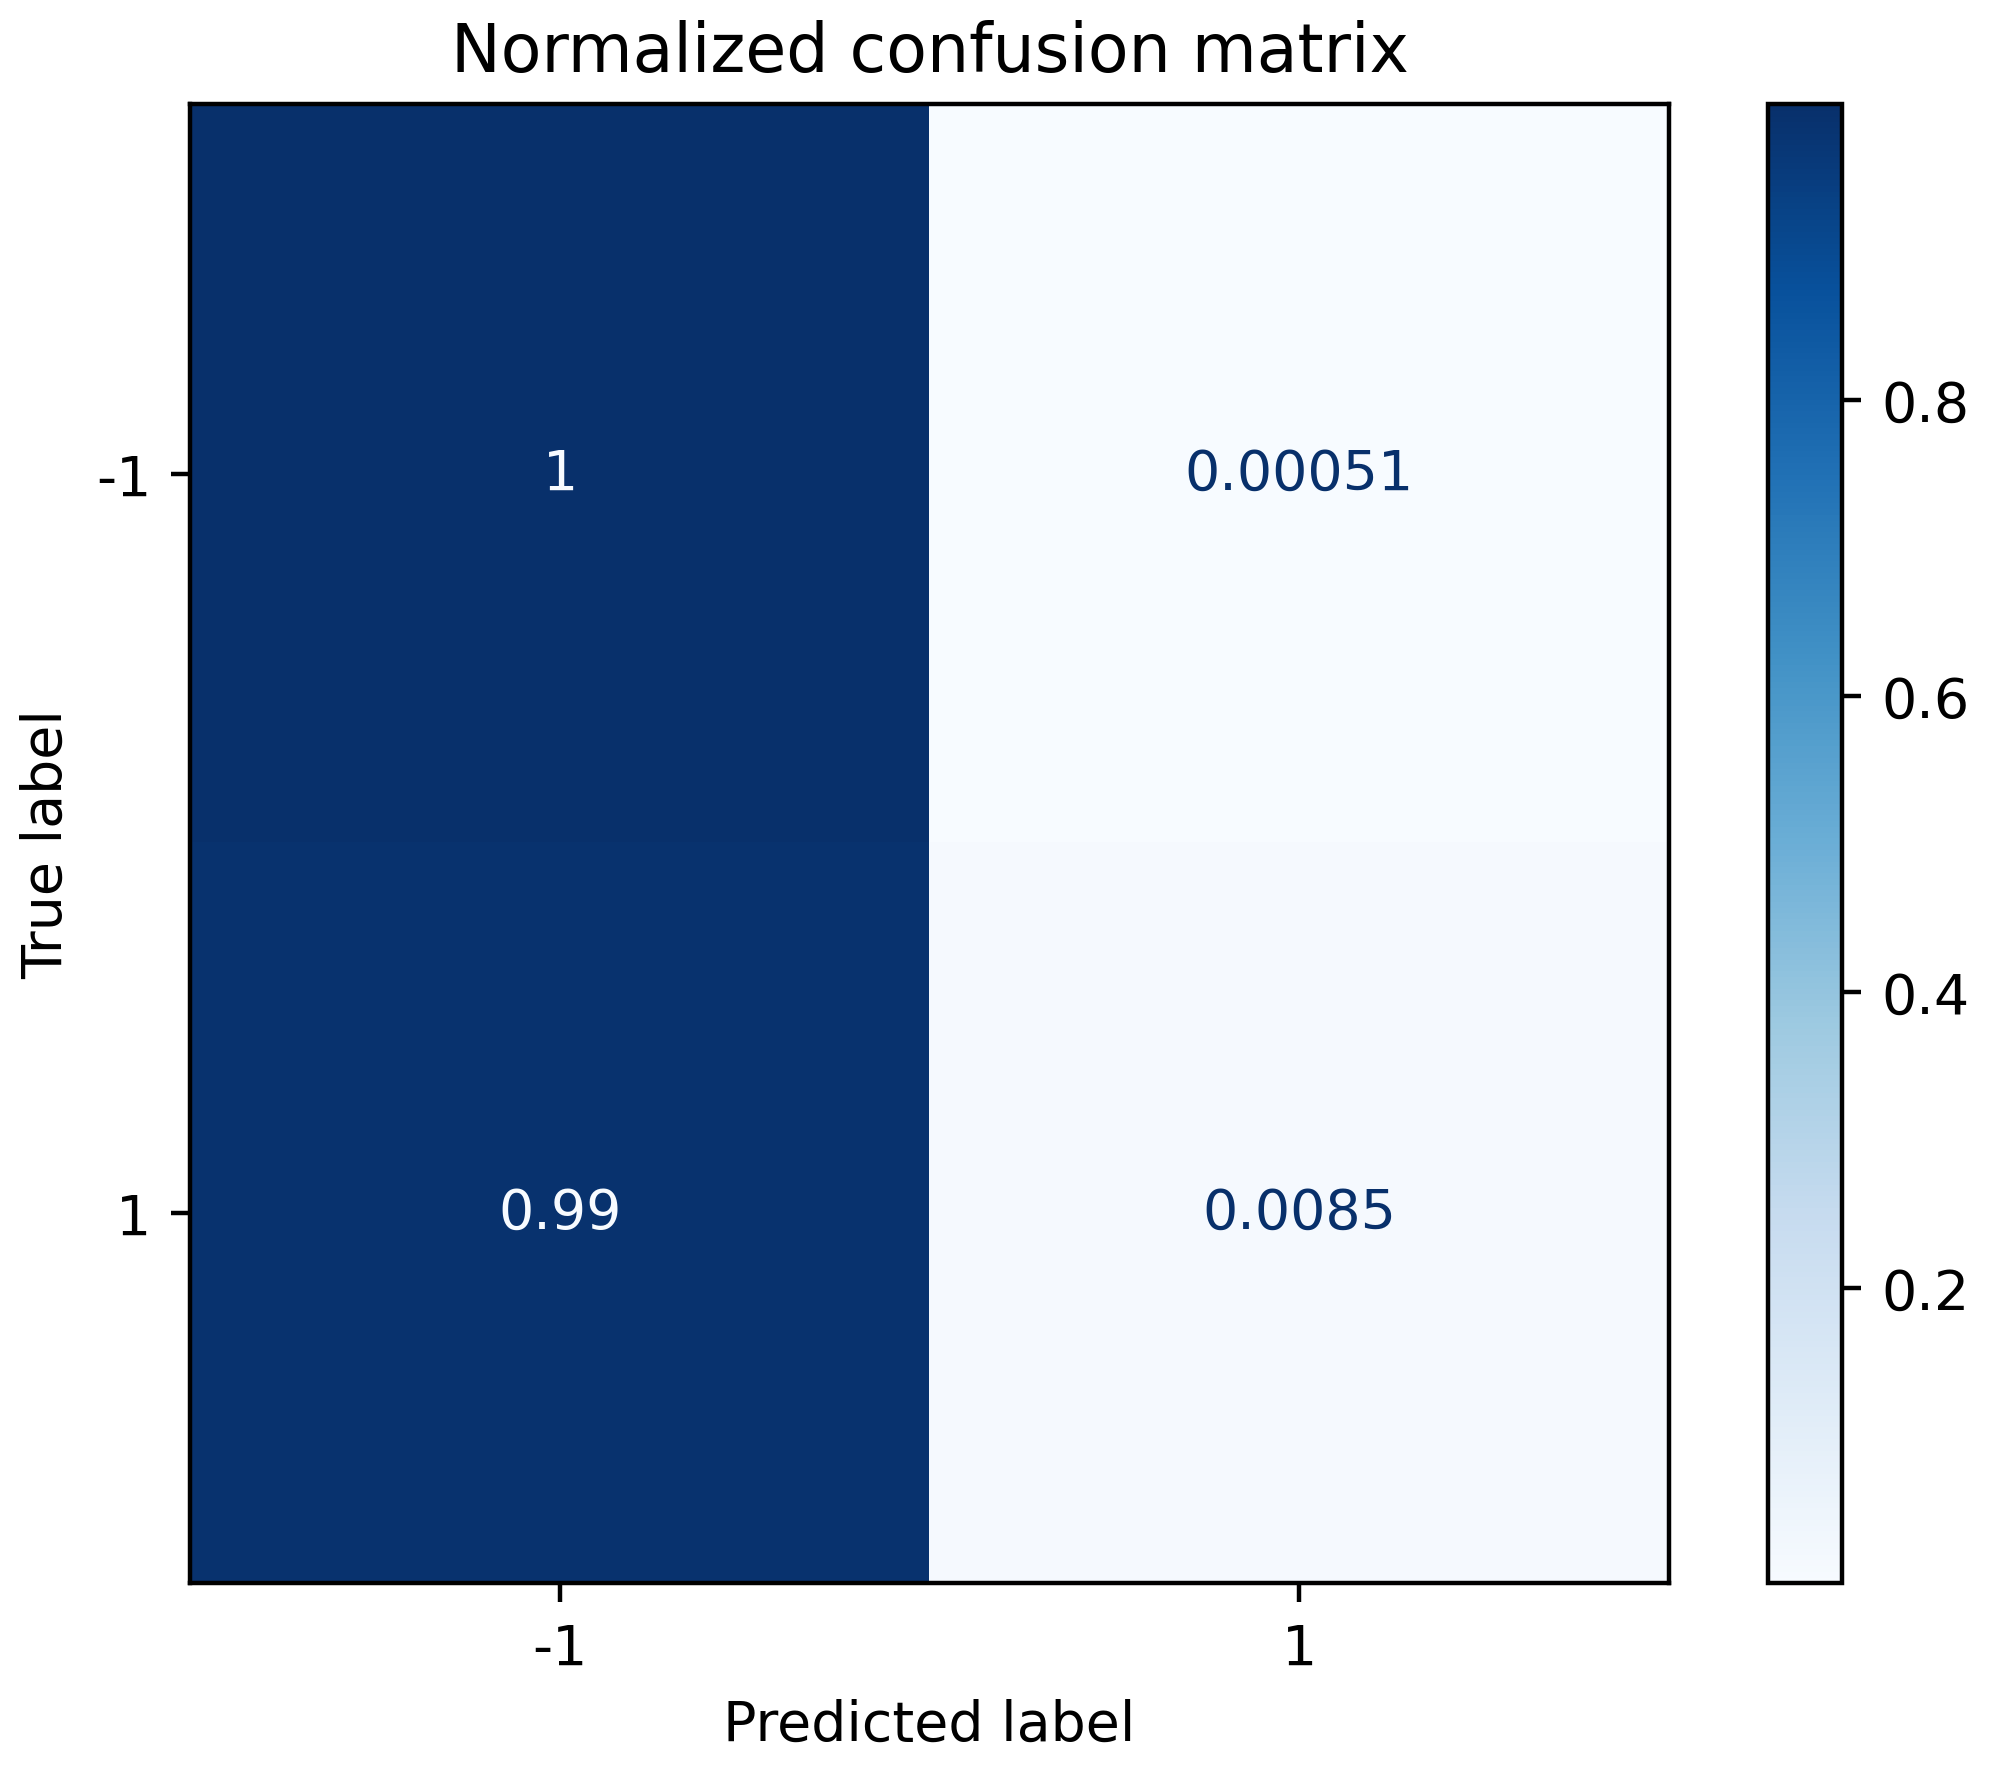
\includegraphics[width=0.48\linewidth]{AdaBoost_confus_mat-norm.png}
    \caption{AdaBoost的混淆矩阵(测试集)}
    \label{fig:result:ada}
\end{figure}

% ============================================================================
\subsubsection{Gradient Boosting}
与AdaBoost算法类似,Gradient Boosting 算法也是 Boosting 下的分支。Boosting 是 Ensemble Learning 算法的一个类别。Boost 的意思为“提升”,这类算法的思想是“给定仅比随机猜测略好的弱学习算法 ,将其提升为强学习算法”。Gradient Boosting 是一种 Boosting 的思想,它本质是,每一次建立模型是在之前建立模型损失函数的梯度下降方向。

同样的,Gradient Boosting 需要调整的参数也是类似的,比如:\texttt{n\_estimators}和\texttt{learning\_rate}。

\begin{itemize}
    \item \texttt{loss}:损失函数。分类模型和回归模型的损失函数是不一样的。

    对于分类模型,有对数似然损失函数"deviance"和指数损失函数"exponential"两者输入选择。默认是对数似然损失函数"deviance"。在原理篇中对这些分类损失函数有详细的介绍。一般来说,推荐使用默认的"deviance"。它对二元分离和多元分类各自都有比较好的优化。而指数损失函数等于把我们带到了Adaboost算法。
\end{itemize}

从表\ref{tb:grad}和图\ref{fig:result:grad}可以看出,相似的结果相对于前面的模型在少数类的表现非常差。

\begin{table}[!h]
    \centering
    \renewcommand{\arraystretch}{1.5}
    \begin{tabular}{|r|c|c|c|}
        \hline
                  & Precision & Recall & F1-score \\ \hline
        -1        &     0.94391     &     0.99847   &    0.97042      \\ \hline
        1         &     0.25000      &     0.00855   &   0.01653       \\ \hline
        macro avg &      0.59695     &     0.50351   &    0.49347      \\ \hline
    \end{tabular}
    \caption{GradientBoosting 的评价}
    \label{tb:grad}
\end{table}

\begin{figure}[!h]
    \centering
    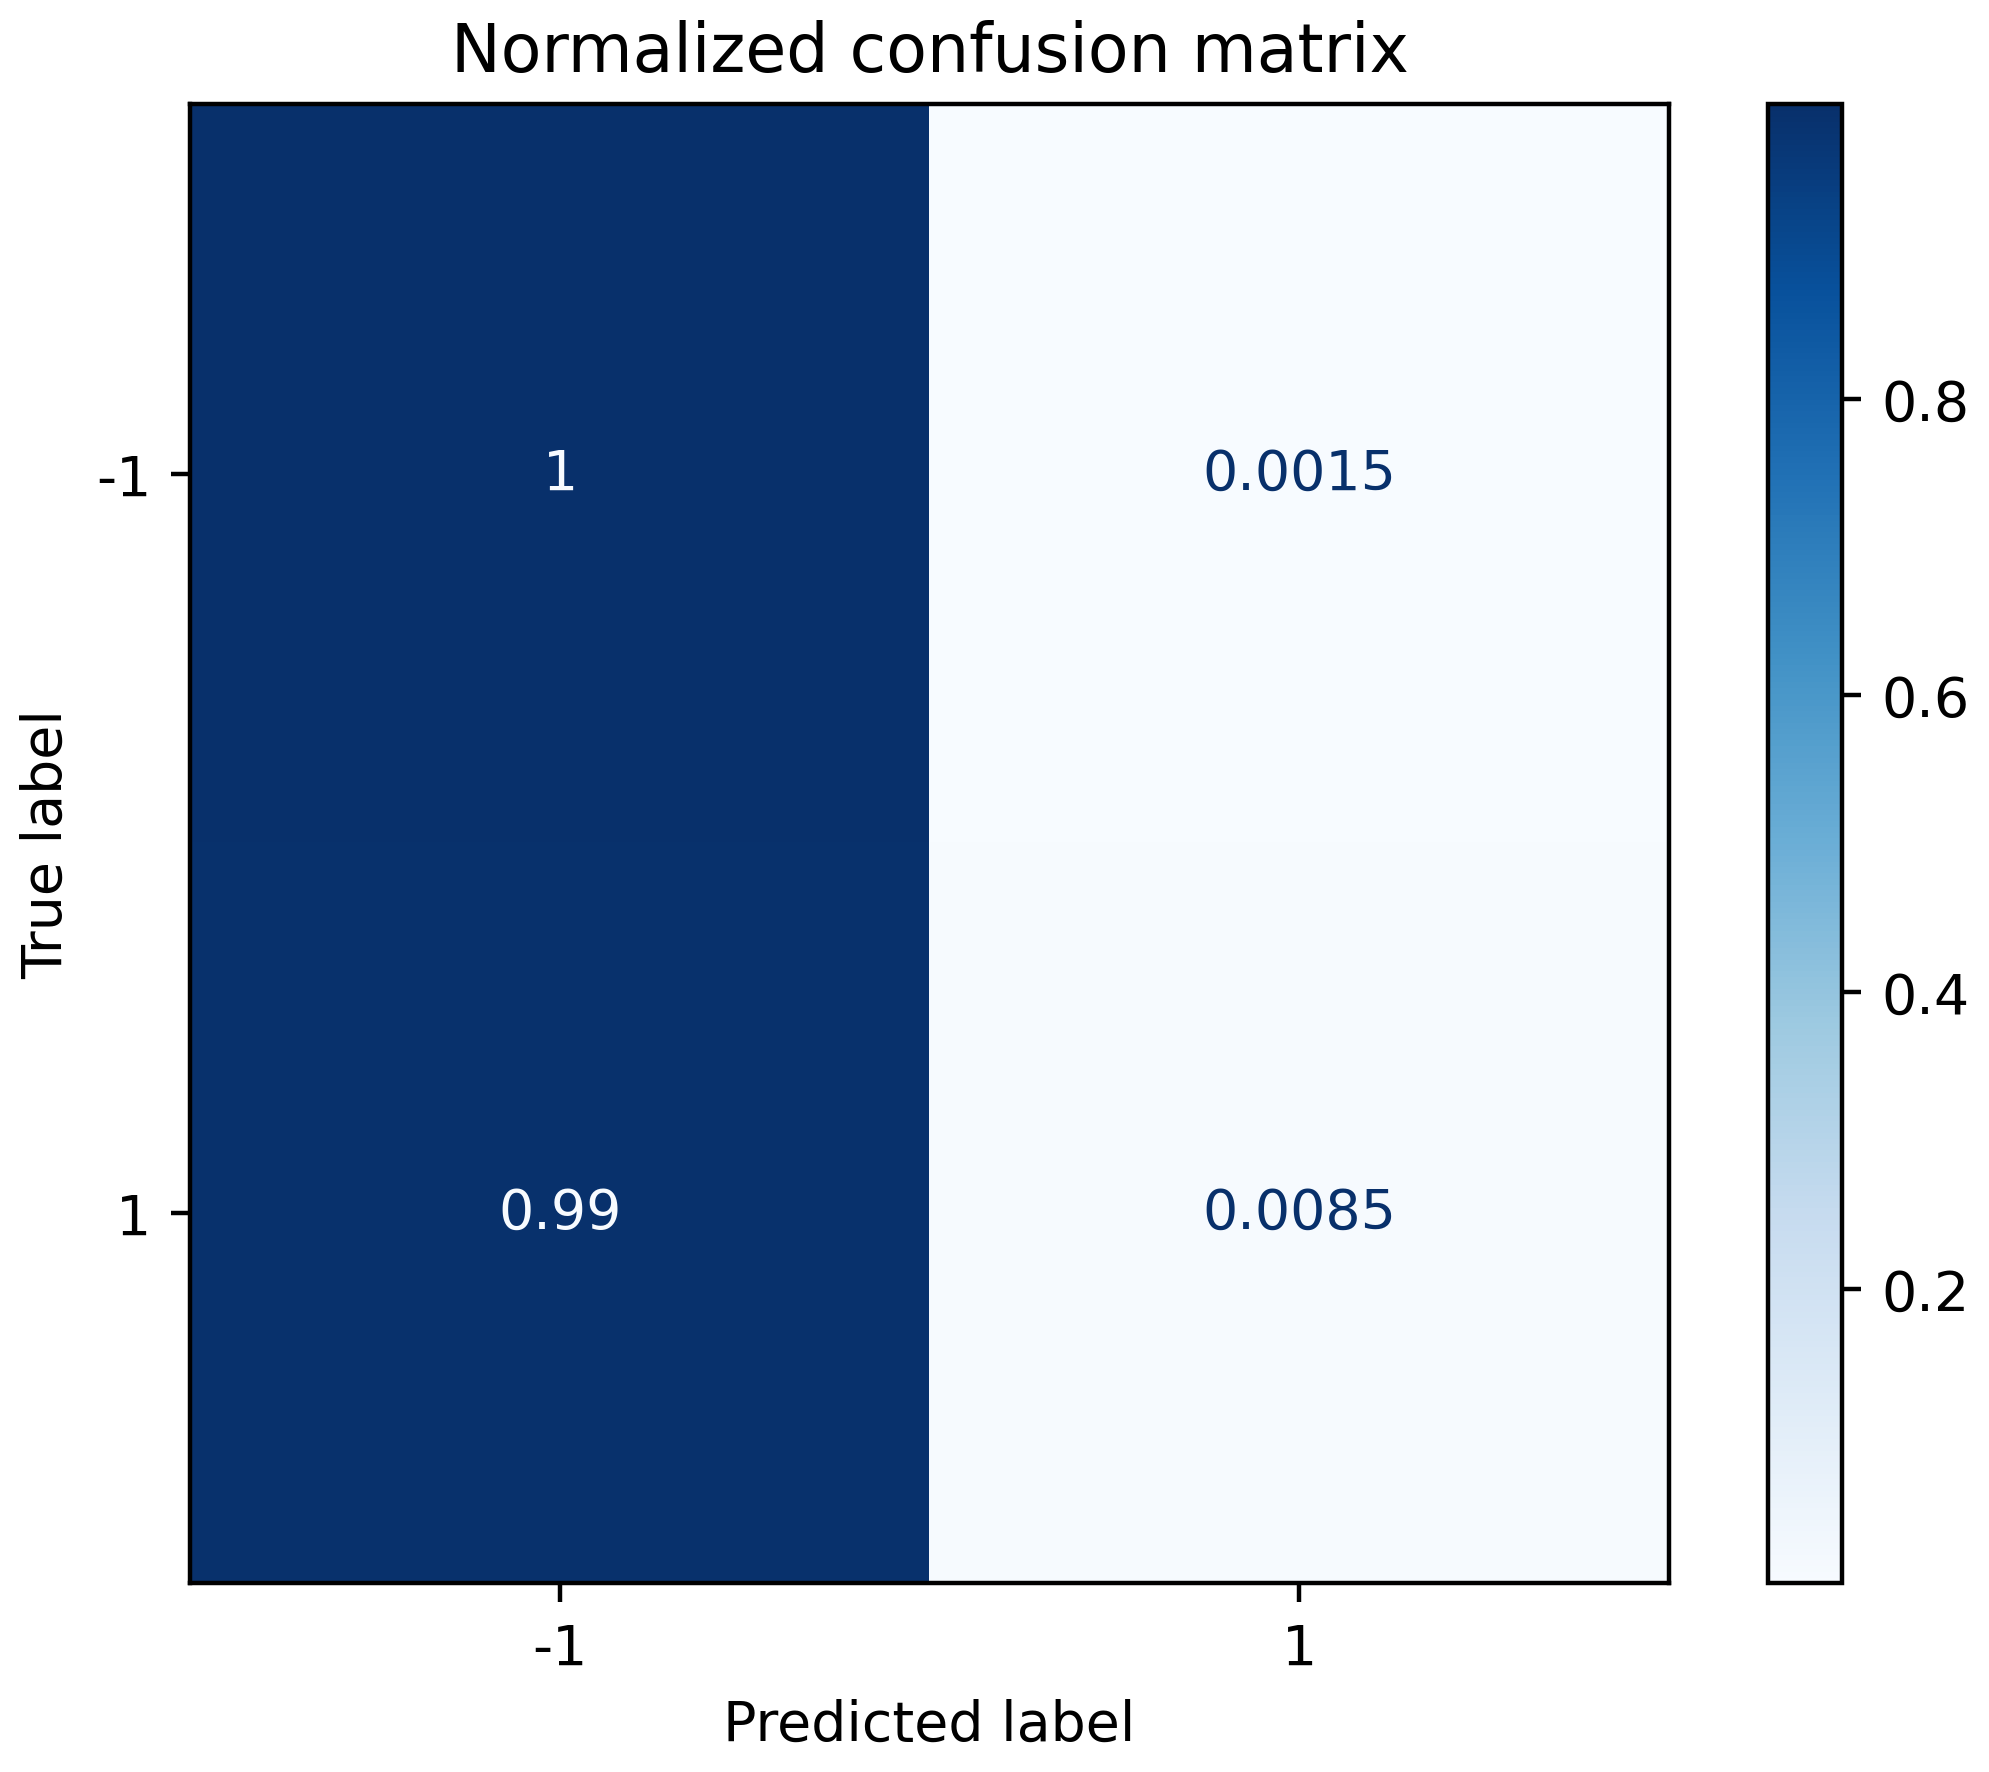
\includegraphics[width=0.48\linewidth]{GradientBoosting_confus_mat-norm.png}
    \caption{GradientBoosting 的混淆矩阵(测试集)}
    \label{fig:result:grad}
\end{figure}

% ============================================================================
% [机器学习] Boosting算法4 --- LightGBM 介绍 
% https://blog.csdn.net/zwqjoy/article/details/90670768
% XGBoost和LightGBM的参数以及调参
% https://www.jianshu.com/p/1100e333fcab
\subsubsection{LightGBM}
LightGBM 是一种基于决策树的Gradient Boosting框架\cite{ke2017lightgbm},2017年由微软提出。在梯度提升决策树(Gradient Boosting Decision Tree, GBDT)上改进,突出轻量light的思想,加快的训练速度,精度却没有损失太多。

使用 \texttt{lightgbm} 中 \texttt{scikit-learn} 接口  -- \texttt{LGBMClassifier}。\texttt{scikit-learn} 接口版本参数和原生参数稍有不同,不过应该无碍。需要调整的重要参数:\texttt{n\_estimators}, \texttt{learning\_rate},
\begin{itemize}
    \item \texttt{boosting\_type}:boosting 类型。默认``gbdt";可选:"gbdt":Gradient Boosting Decision Tree,"dart":Dropouts meet Multiple Additive Regression Trees ,"goss":Gradient-based One-Side Sampling,"rf": Random Forest。
\end{itemize}
根据基础参数 \texttt{class\_weight = `balanced'} , \texttt{objective='binary'}。经过参数搜索,得搜索结果:\texttt{n\_estimators}: 15, \texttt{max\_depth}: 5,得到以下图\ref{fig:result:lgbm}和表\ref{tb:lgbm}。

\begin{table}[!h]
    \centering
    \renewcommand{\arraystretch}{1.5}
    \begin{tabular}{|r|c|c|c|}
        \hline
                  & Precision & Recall & F1-score \\ \hline
        -1        &     0.96985     &     0.77340   &    0.86056      \\ \hline
        1         &     0.13645      &     0.59829   &   0.22222       \\ \hline
        macro avg &      0.55315     &     0.68585   &    0.54139      \\ \hline
    \end{tabular}
    \caption{LightGBM的评价}
    \label{tb:lgbm}
\end{table}

\begin{figure}[!h]
    \centering
    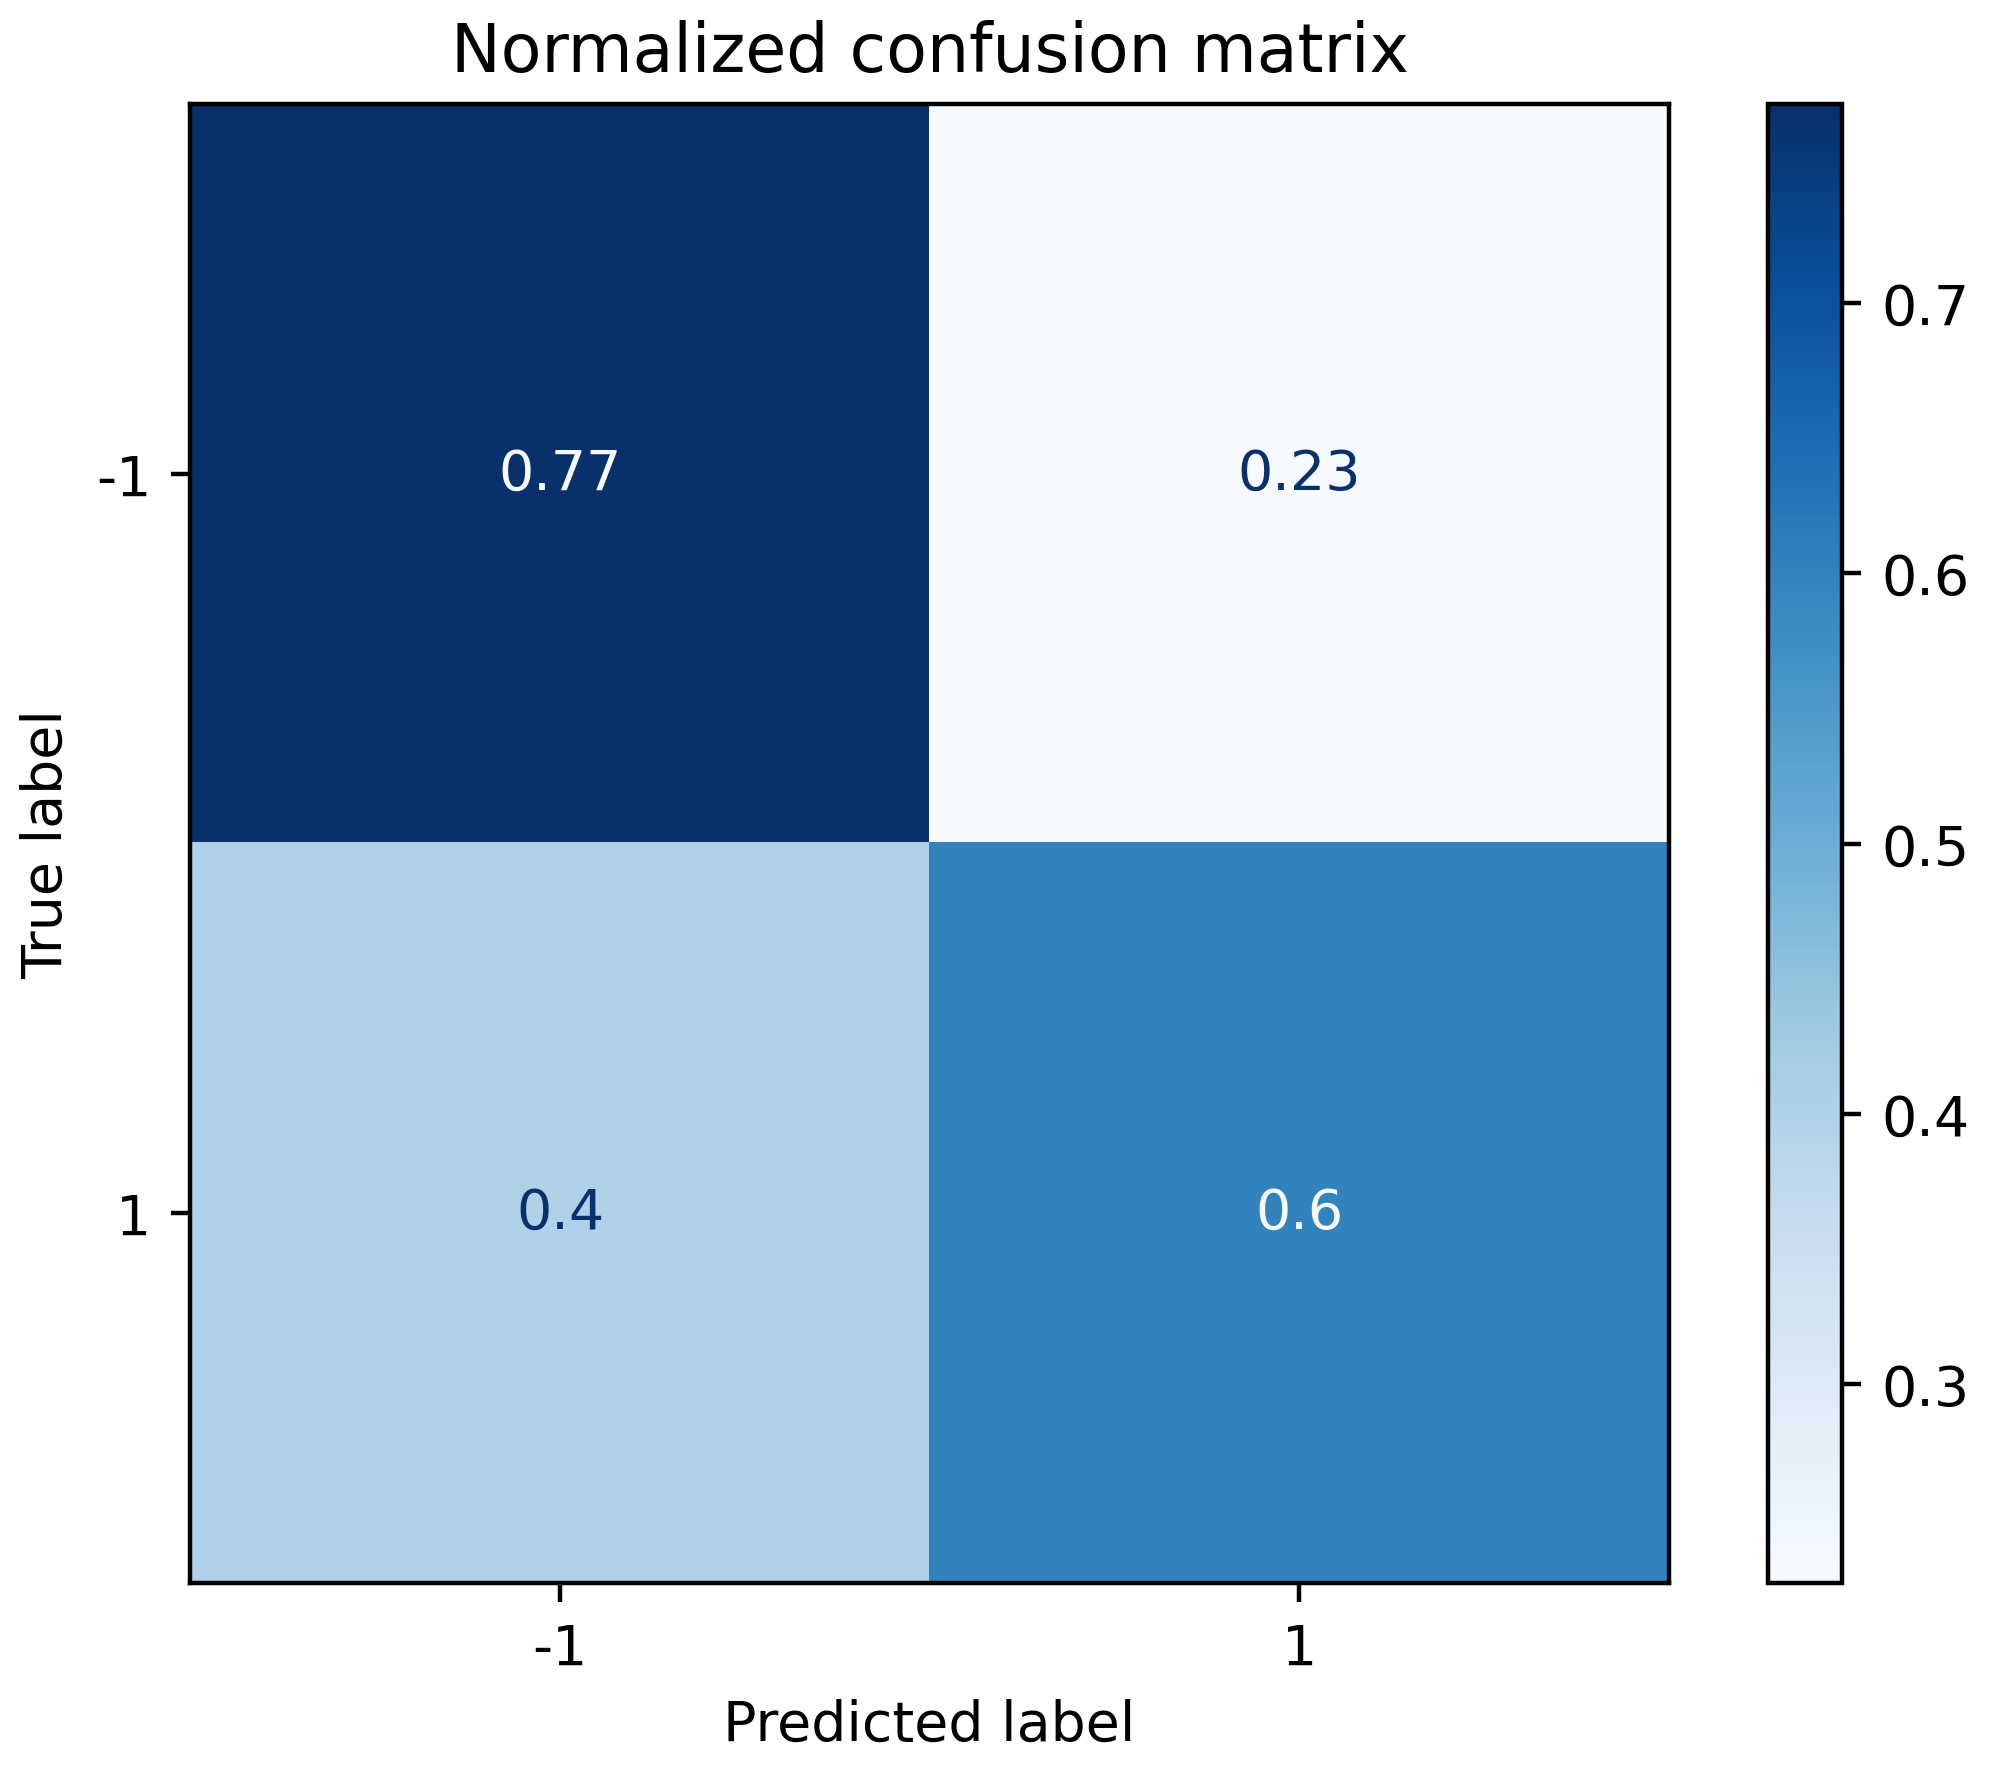
\includegraphics[width=0.48\linewidth]{LightGBM_confus_mat-norm.png}
    \caption{LightGBM的混淆矩阵(测试集)}
    \label{fig:result:lgbm}
\end{figure}


% ============================================================================
\subsubsection{XGBoost}

XGBoost 是陈天奇在2016年提出了一种可扩展性的端到端基于树的Boosting系统 \cite{chen2016xgboost},这个系统可以处理稀疏性数据,通过分布式加权直方图算法去近似学习树,这个系统也提供基于缓存的加速模式、数据压缩、分片功能。

% XGBoost原理和底层实现剖析
% https://snaildove.github.io/2018/10/02/get-started-XGBoost/
% XGBoost 陈天奇论文 ppt 个人总结
% https://zdkswd.github.io/2019/03/04/XGBoost%20%E4%B8%AA%E4%BA%BA%E6%80%BB%E7%BB%93/

% [机器学习] Boosting算法3 --- XGBoost
% https://blog.csdn.net/zwqjoy/article/details/89281846

XGBoost 没有提供 \texttt{class\_weight='balanced'} 参数,但是提供替代参数 \texttt{scale\_pos\_weight},控制正负类权重的平衡,提供一个 \texttt{float} 值,典型的计算方式是 \texttt{sum(negative instances) / sum(positive instances)}。

使用 \texttt{xgboost} 中 \texttt{scikit-learn} 接口  -- \texttt{XGBClassifier}。需要调整的重要参数:\texttt{n\_estimators}, \texttt{max\_depth}。这两个参数前面模型已有解释,故这里不再解释。


根据设定的基础参数 \texttt{scale\_pos\_weight} 经过参数搜索,搜索结果为:\texttt{n\_estimators}: 90, \\\texttt{max\_depth}: 9,得到以下图\ref{fig:result:xgb}和表\ref{tb:xgb}。

\begin{table}[!h]
    \centering
    \renewcommand{\arraystretch}{1.5}
    \begin{tabular}{|r|c|c|c|}
        \hline
                  & Precision & Recall & F1-score \\ \hline
        -1        &     0.95942     &     0.81023   &    0.87854      \\ \hline
        1         &     0.11876      &     0.42735   &   0.18587       \\ \hline
        macro avg &      0.53909     &     0.61879   &    0.53220      \\ \hline
    \end{tabular}
    \caption{XGBoost 的评价}
    \label{tb:xgb}
\end{table}

\begin{figure}[!h]
    \centering
    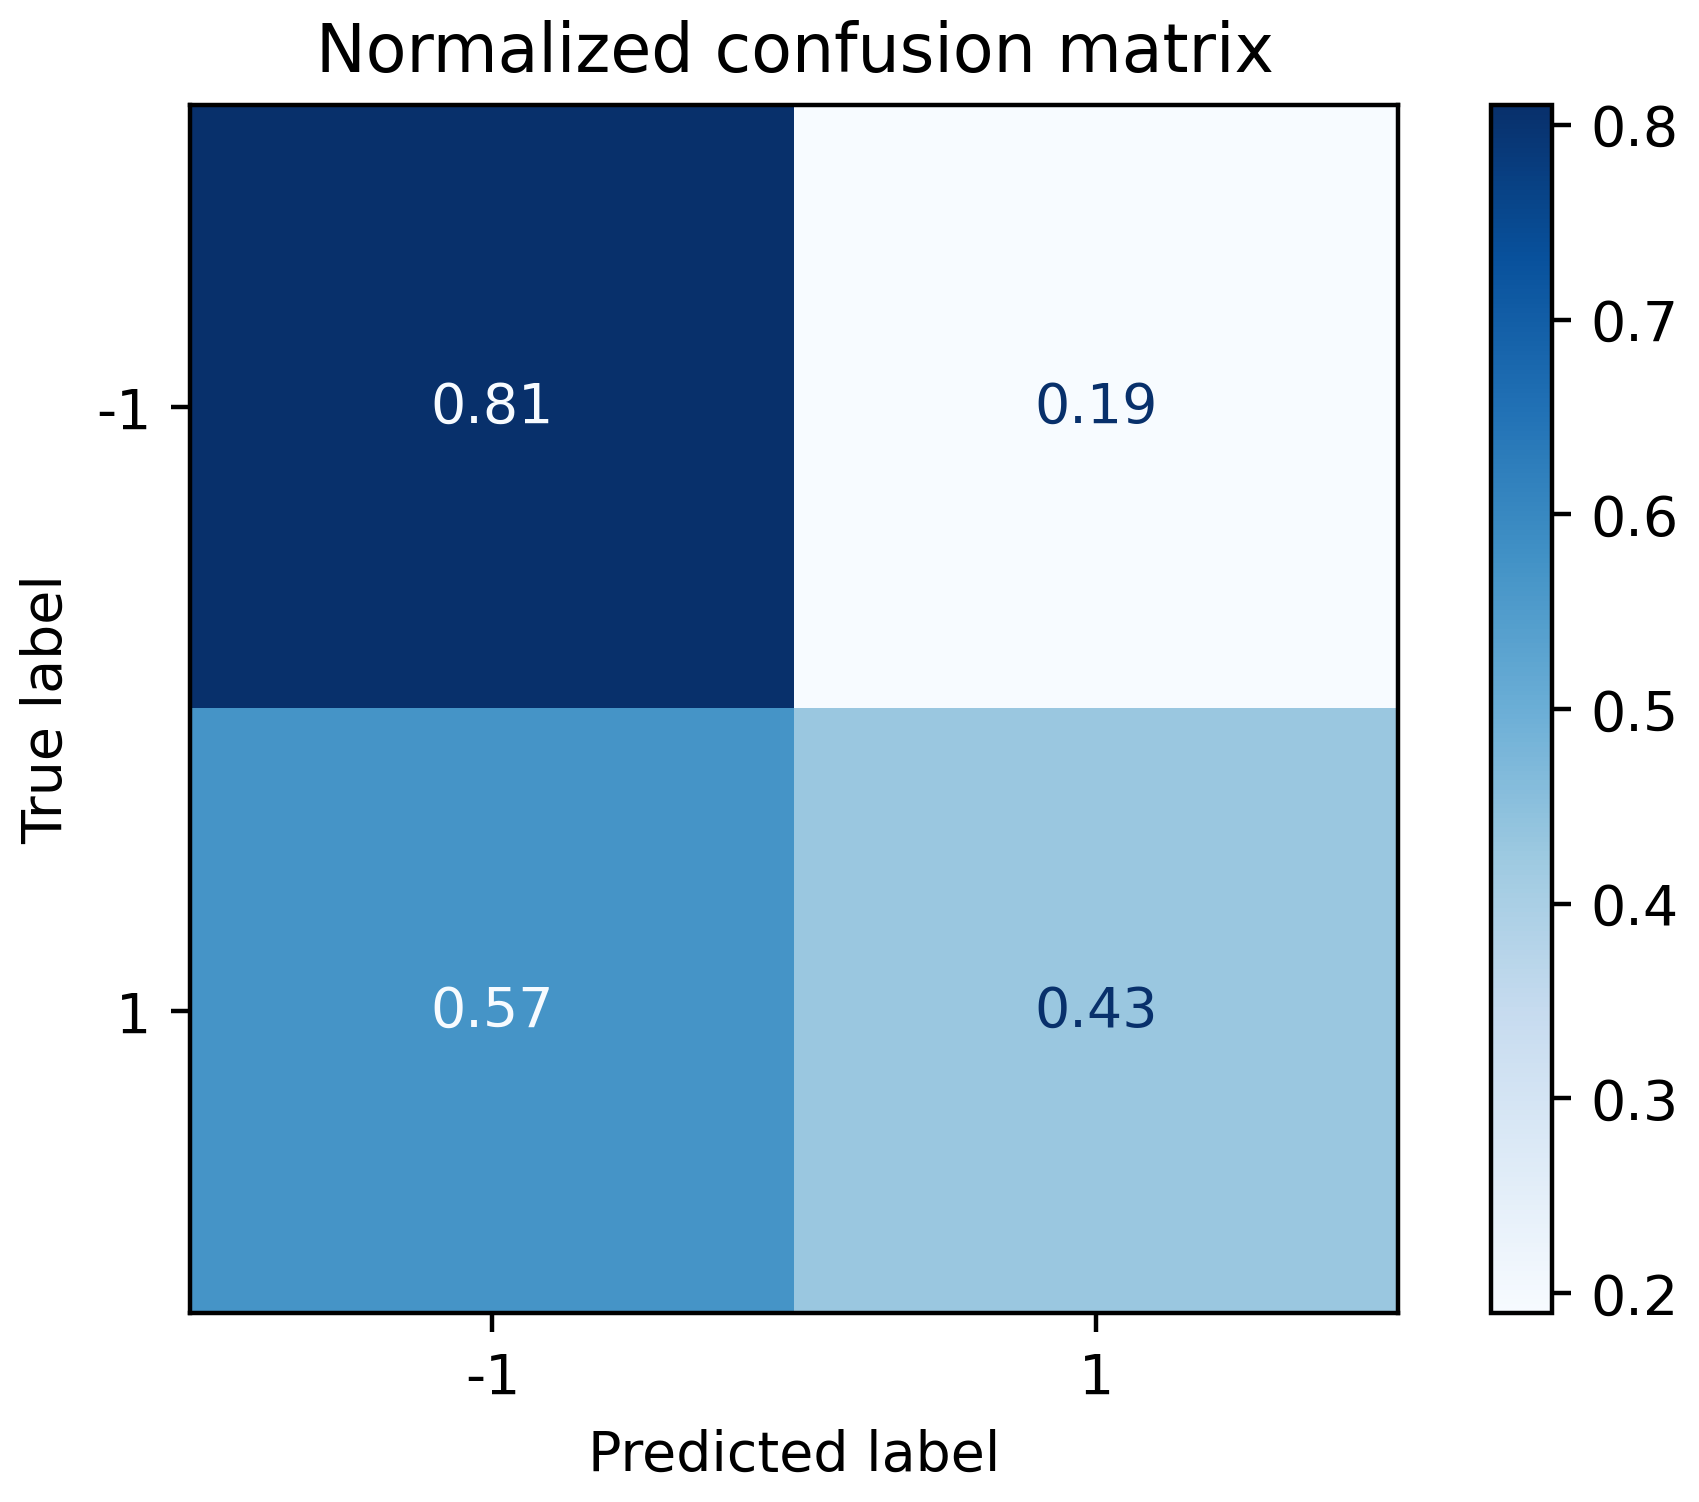
\includegraphics[width=0.48\linewidth]{xgboost_confus_mat-norm.png}
    \caption{XGBoost 的混淆矩阵(测试集)}
    \label{fig:result:xgb}
\end{figure}


% ============================================================================
\subsection{模型效果对比}

模型效果对比均进行了过采样或者设定了\texttt{class\_weight='balanced'}参数等 类似的平衡少数类的的措施。正类(少数类),precision、recall、F1分数最好的分类器分别是线性SVM、AdaBoost、线性SVM。简单的模型反而相对表现好。但是总体上来说,少数类的准确率在13\%左右,召回率在56\%,F1分数在21\%。

负类(多数类)本身在测试样本上就有优势,不同分类器在召回率表现都差异不大;在召回率上就区别较大了,表现最好还是线性SVM,其次是XGBoost;在F1分数上前两位也服从这个排序。总体上来说,多数类的准确率在96\%左右,召回率在77\%,F1分数在85\%。

如果需要兼顾正类和负类的表现,宏平均值(类表现的算术平均数)是一种度量。只看准确率或F1分数线性SVM是最好的,只看召回率随机森林是最好的。对于不同分类器来说,平均准确率在13\%左右,平均召回率在56\%,平均F1分数在21\%,相对差异不是太大。


GBDT 和 LightGBM 结果表现非常接近,这可以理解,因为 LightGBM 是在 GBDT 上改进的,但是可能数据质量或者数量不过无法体现 LightGBM 的改进之处。

\begin{figure}[!h]
    \centering
    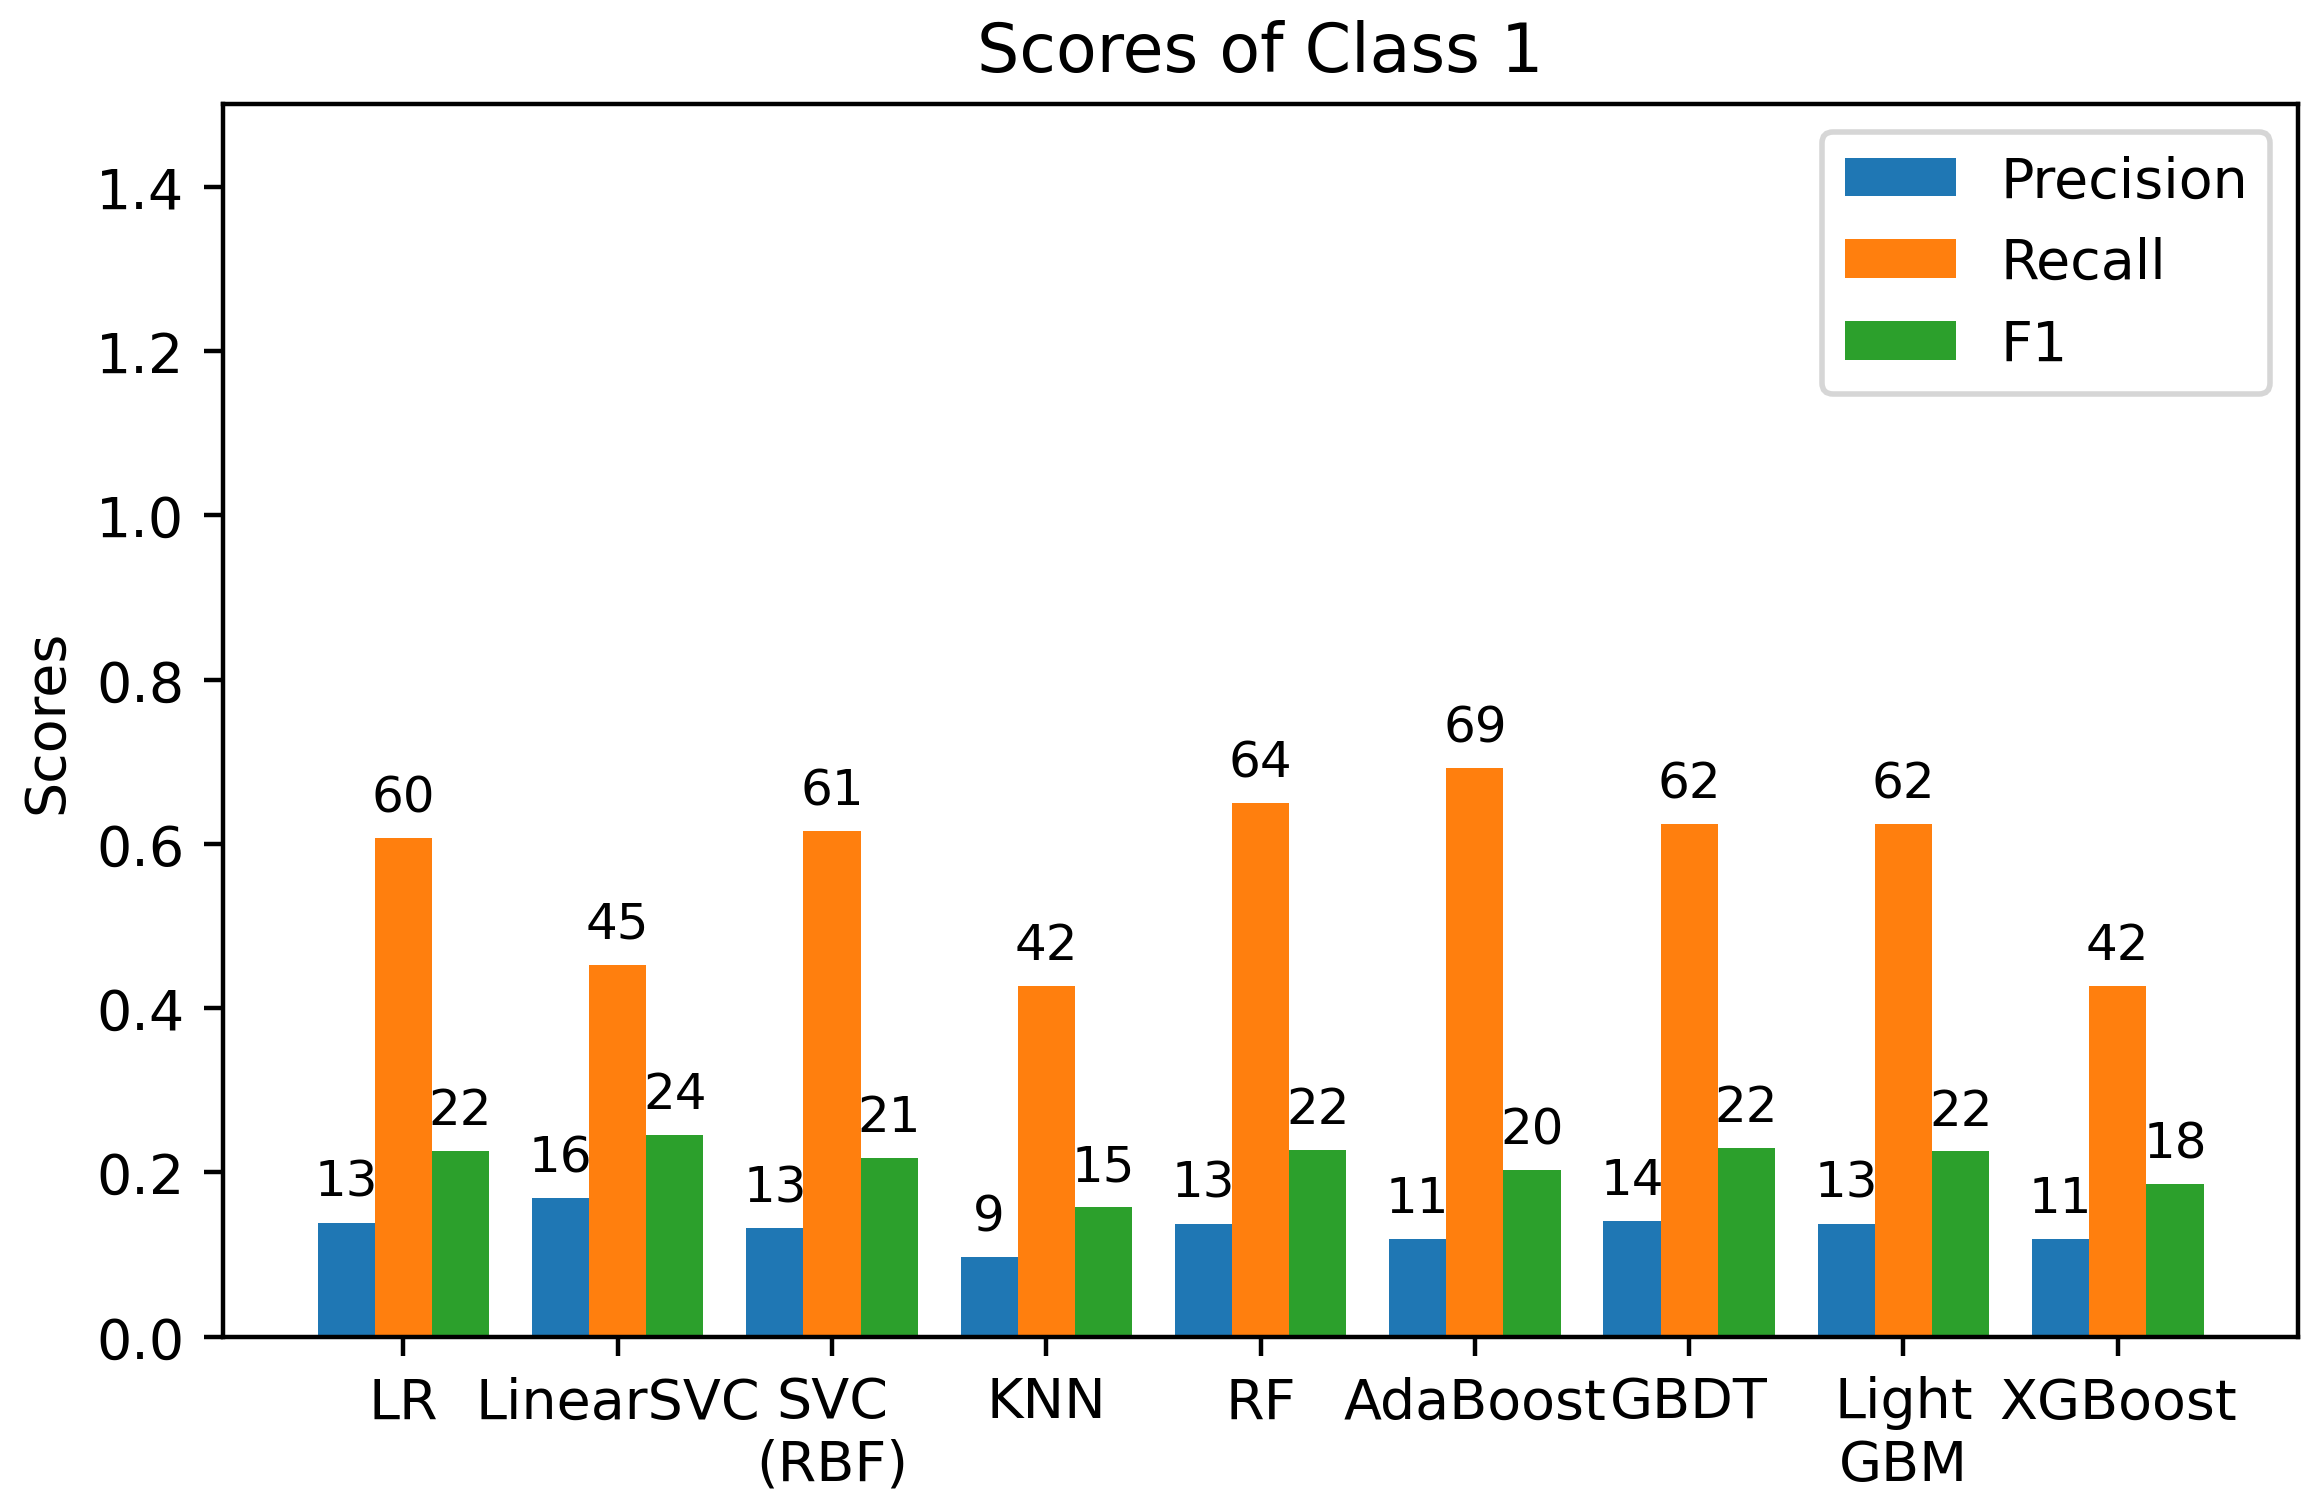
\includegraphics[width=0.8\linewidth]{pos.png}
    \caption{正类(少数类)在不同分类器上的表现}
    \label{fig:result:pos}
\end{figure}


\begin{figure}[!h]
    \centering
    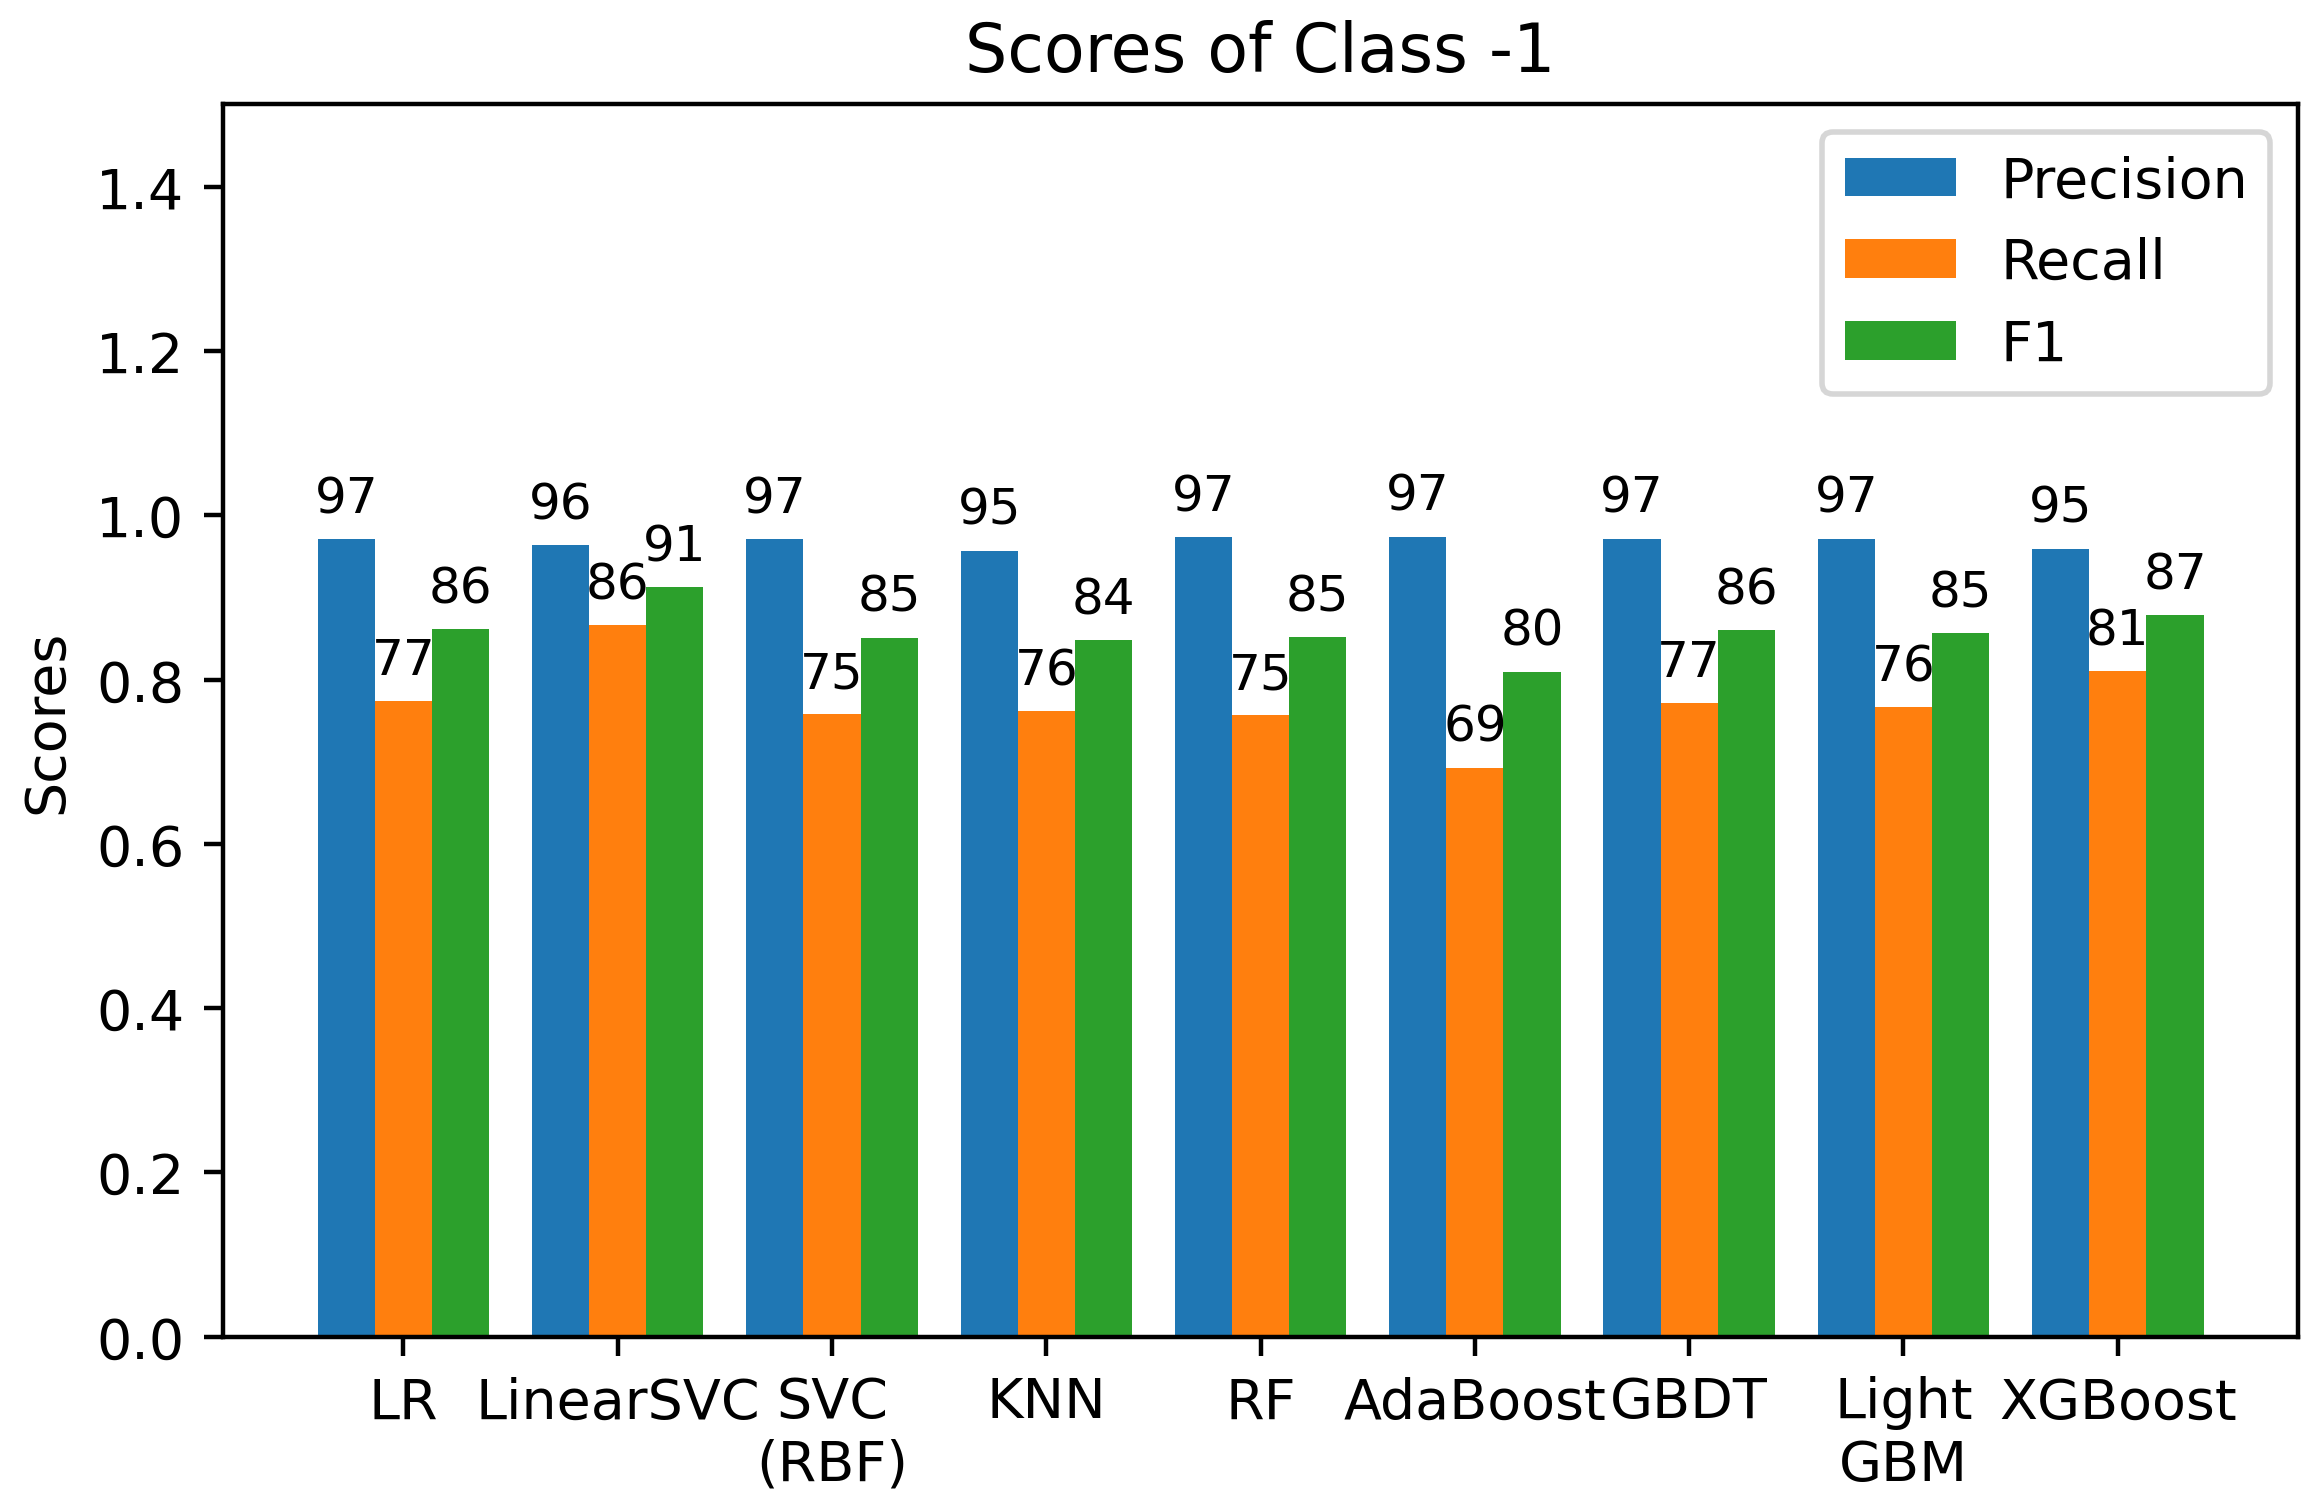
\includegraphics[width=0.8\linewidth]{neg.png}
    \caption{负类(多数类)在不同分类器上的表现}
    \label{fig:result:neg}
\end{figure}

\begin{figure}[!h]
    \centering
    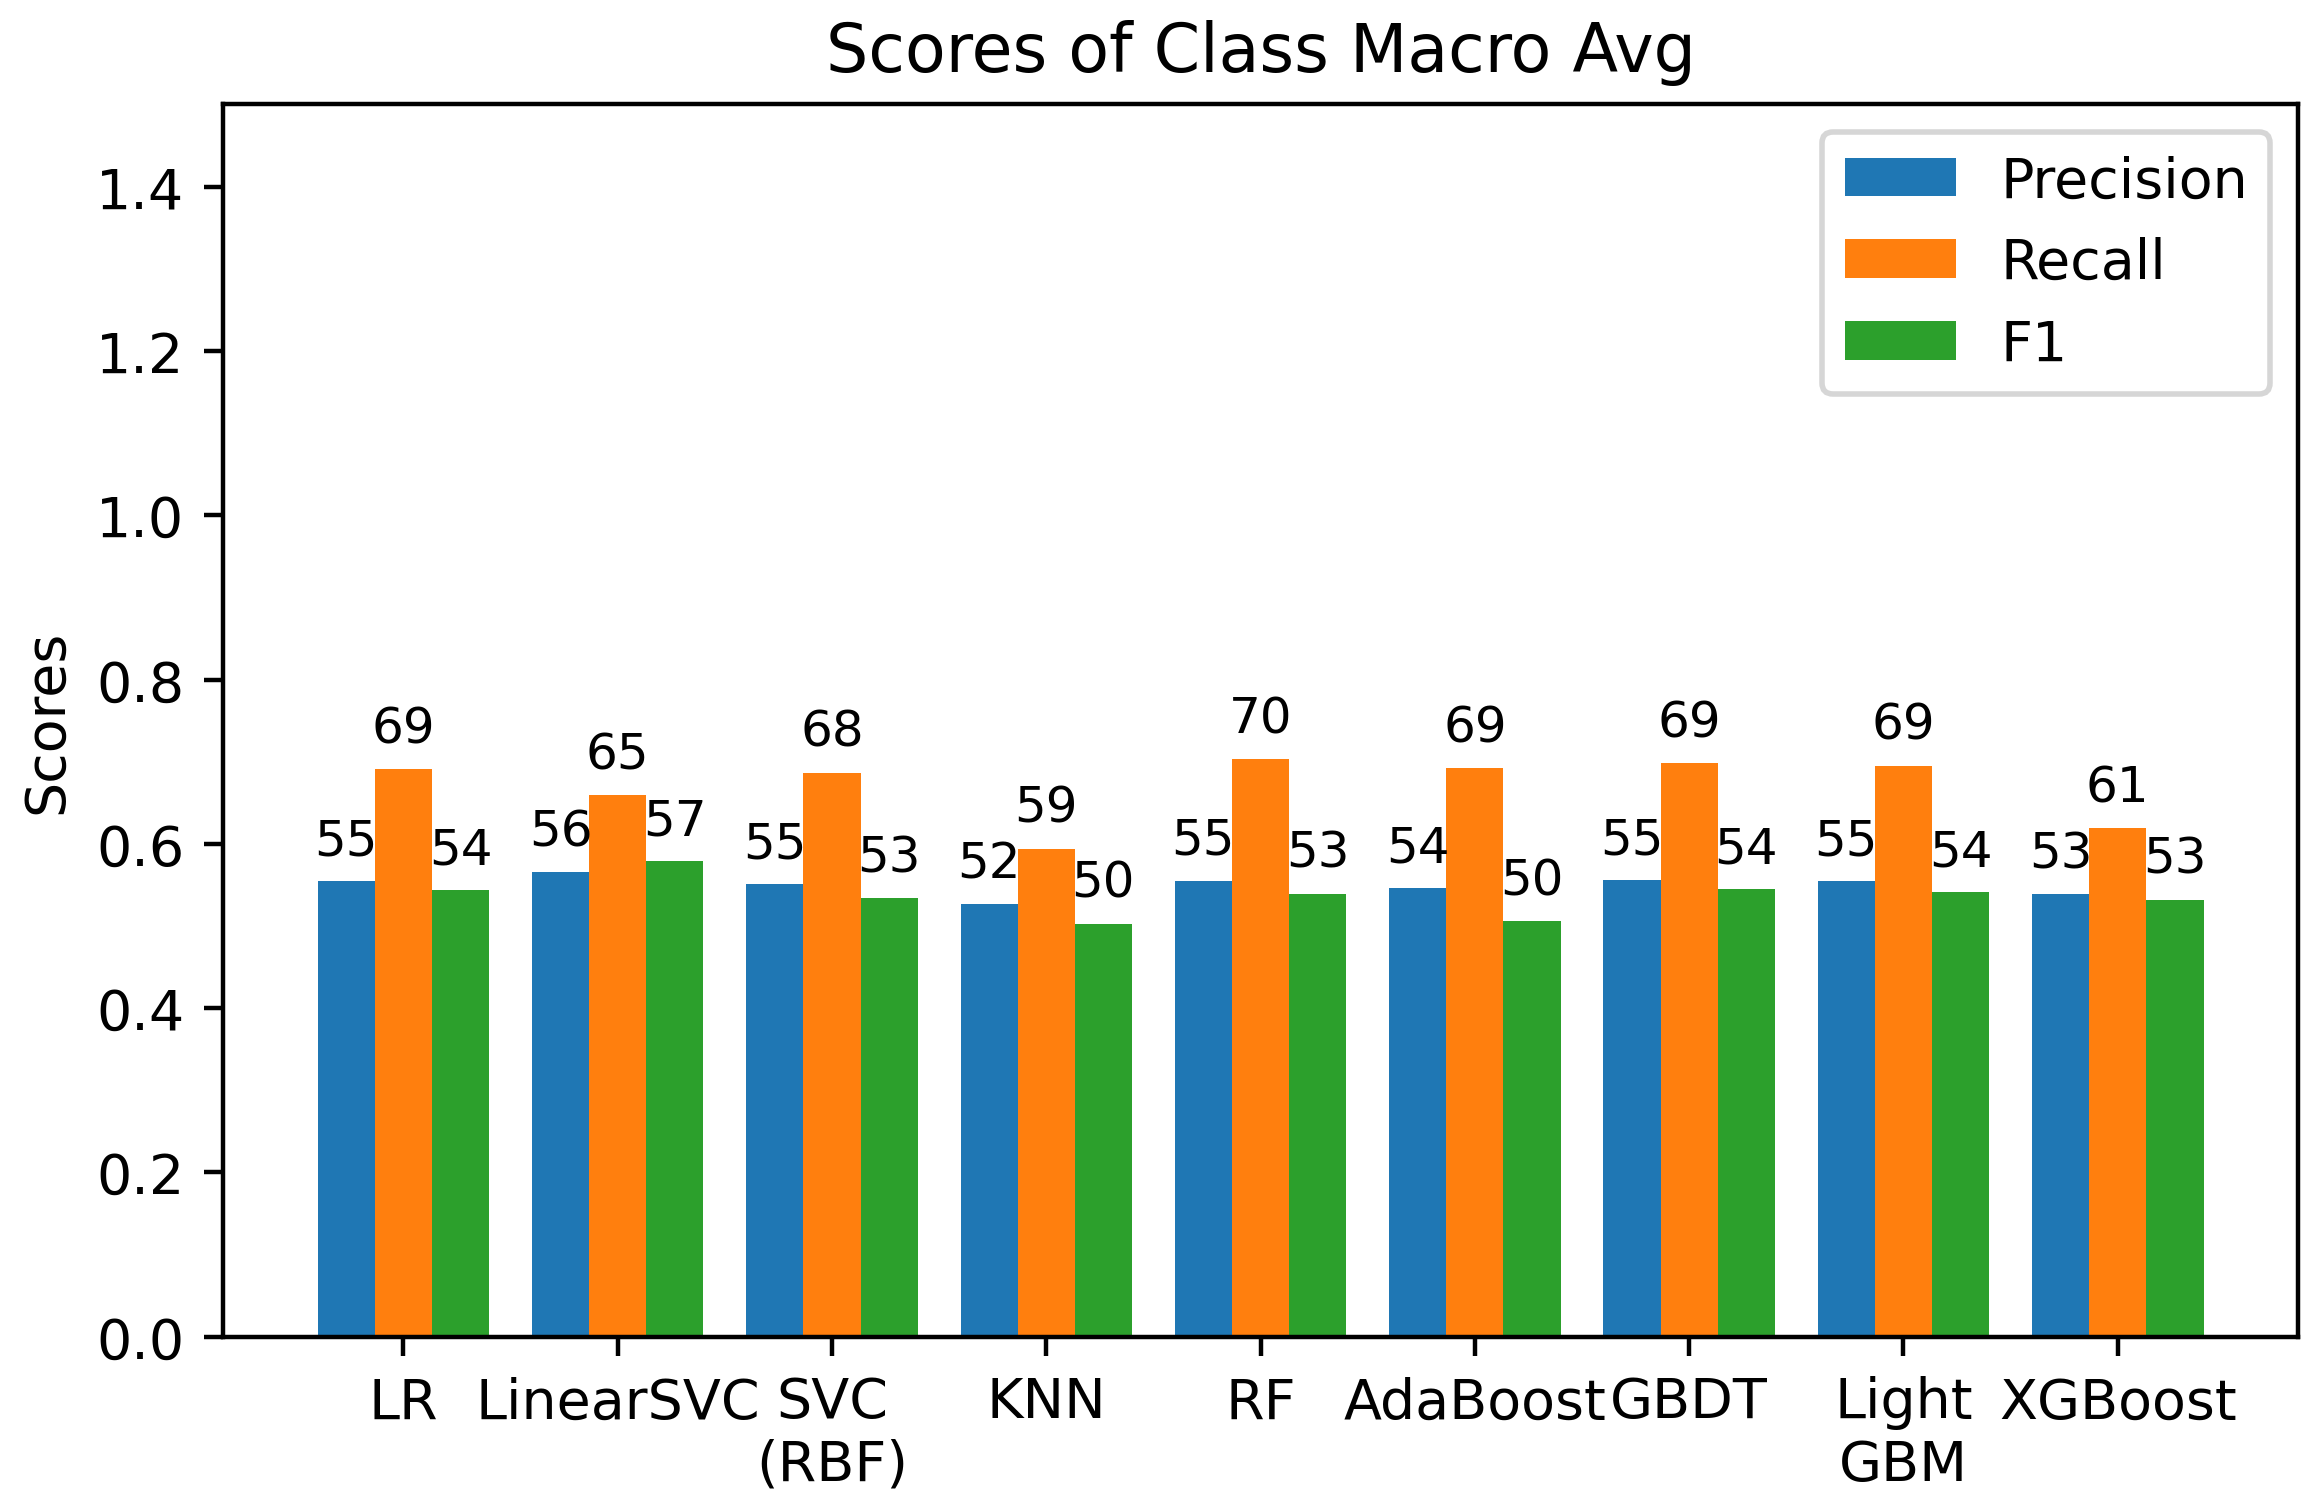
\includegraphics[width=0.8\linewidth]{avg.png}
    \caption{宏平均值(类表现的算术平均数)在不同分类器上的表现}
    \label{fig:result:avg}
\end{figure}


\clearpage
\subsection{过采样效果对比}
\label{sec:resample}

\subsubsection{无调整 vs. 过采样}

前面有些模型在训练时候没有可选参数(\texttt{class\_weight='balanced'})。因为没有针对不平衡类优化,所以少数类表现特别差。下面使用过采样的方式实验是否能提高少数类的性能。

例如最近邻算法,应用SMOTE,结果如图\ref{fig:result:knn-re}和表\ref{tb:knn-re},与没有使用过采样的图\ref{fig:result:knn}和表\ref{tb:knn}相比,平均类准确率和召回率具有提升,在提升少数类表现的同时,多数类表现下降,这是放大少数类噪声造成的影响。

\begin{table}[!h]
    \centering
    \renewcommand{\arraystretch}{1.5}
    \begin{tabular}{|r|c|c|c|}
        \hline
                  & Precision & Recall & F1-score \\ \hline
        -1        &     0.95691     &     0.76113   &    0.84786      \\ \hline
        1         &     0.09671      &     0.42735   &   0.15773       \\ \hline
        macro avg &      0.52681     &     0.59424   &    0.50280      \\ \hline
    \end{tabular}
    \caption{使用SMOTE过采样和KNN的评价}
    \label{tb:knn-re}
\end{table}


\begin{figure}[!ht]
\centering
\begin{minipage}[t]{0.48\textwidth}
\centering
    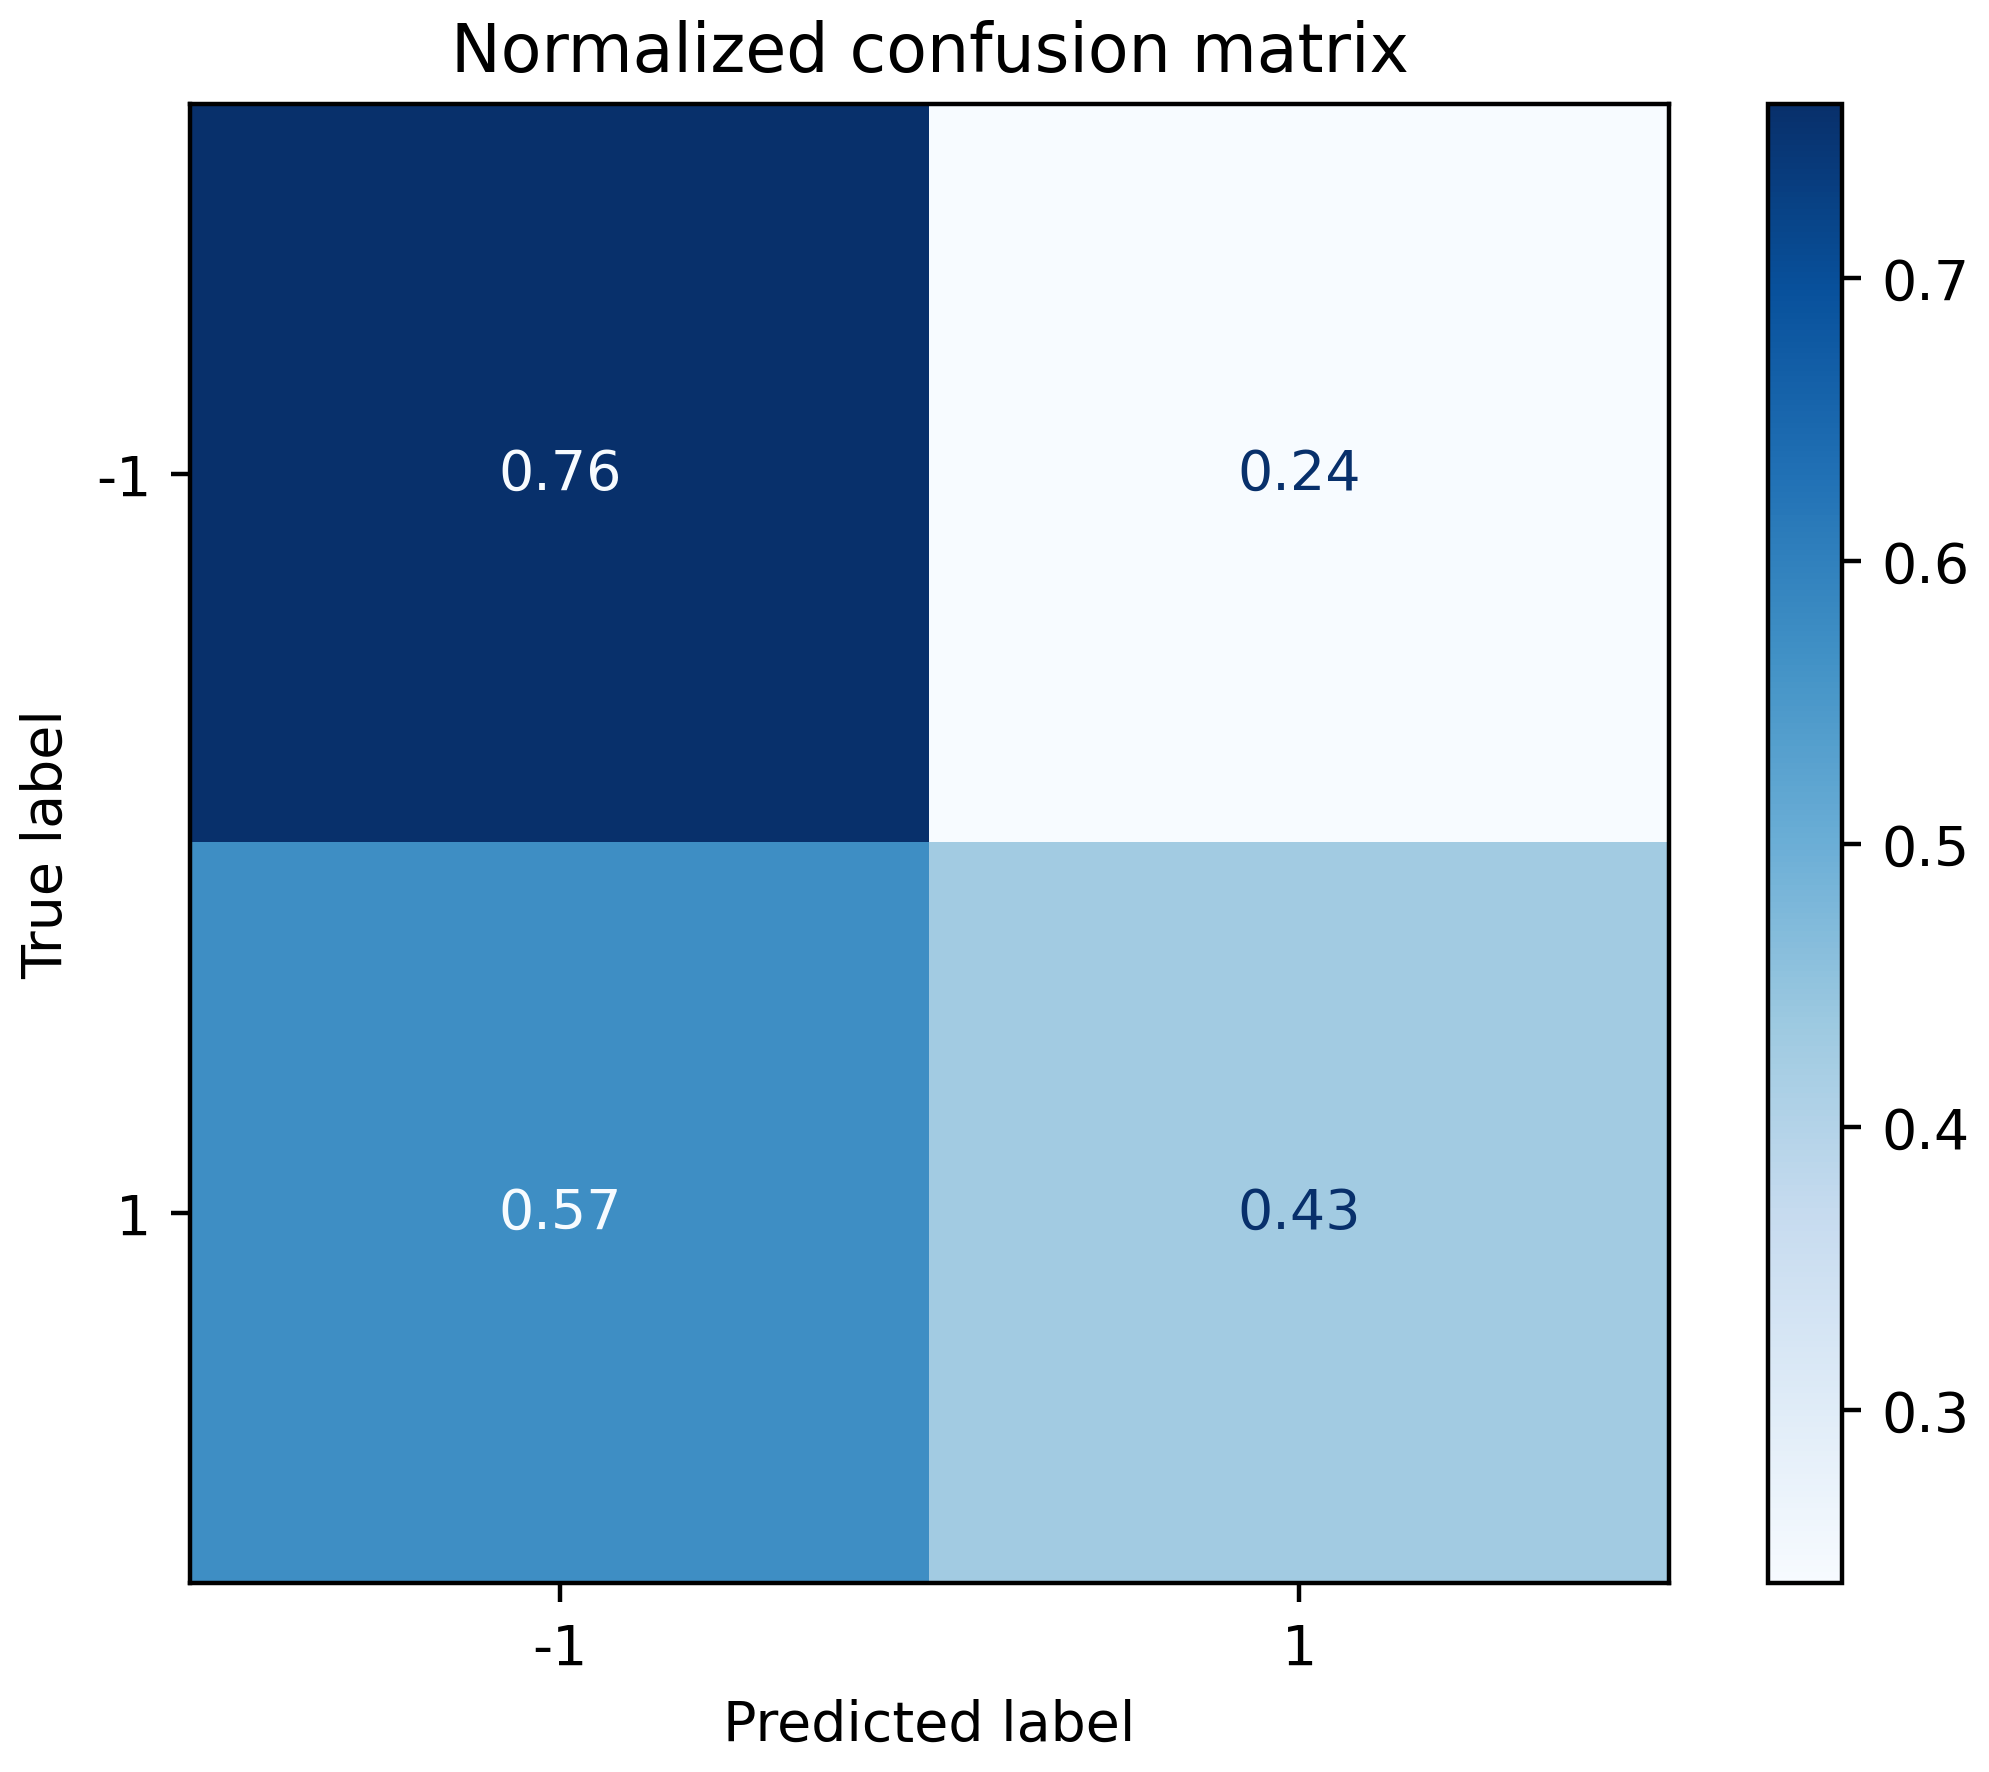
\includegraphics[width=\linewidth]{KNN-re_confus_mat-norm.png}
    \caption{使用SMOTE过采样和KNN的混淆矩阵(测试集)}
    \label{fig:result:knn-re}
\end{minipage}\hfill%
\begin{minipage}[t]{0.48\textwidth}
\centering
    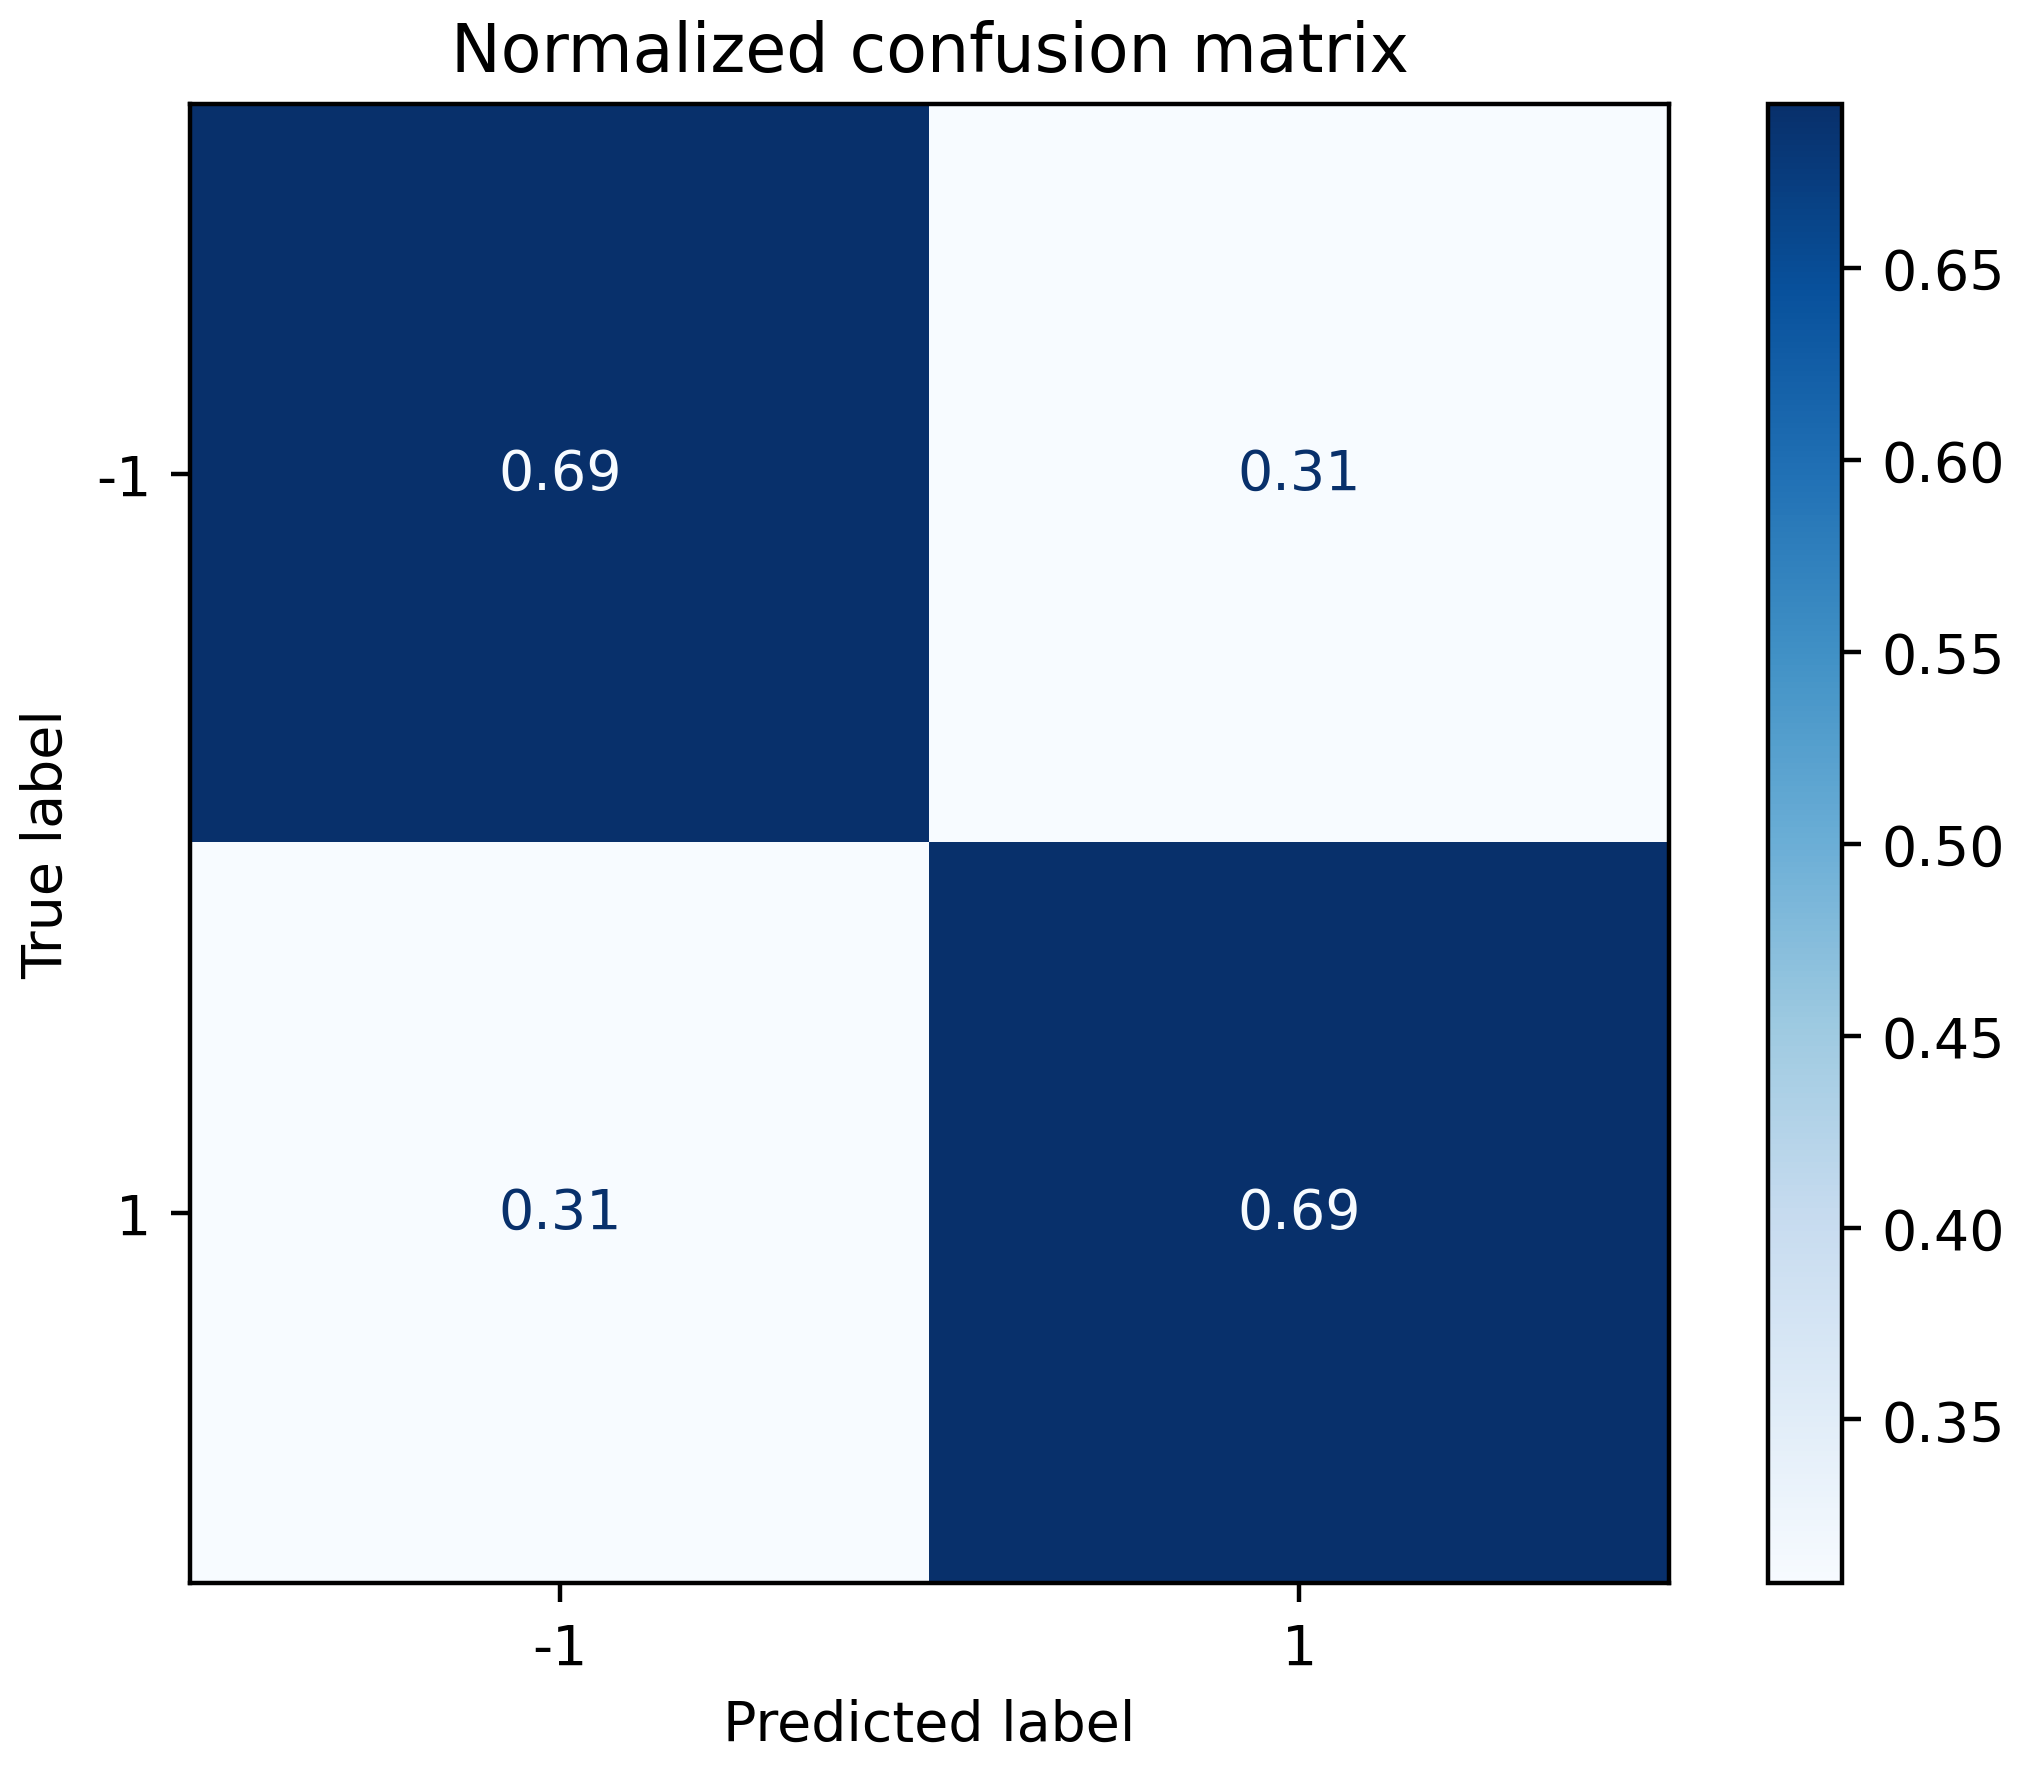
\includegraphics[width=\linewidth]{AdaBoost-re_confus_mat-norm.png}
    \caption{使用SMOTE过采样和AdaBoost的混淆矩阵(测试集)}
    \label{fig:result:ada-re}
\end{minipage}
\end{figure}

% \begin{figure}[!h]
%     \centering
%     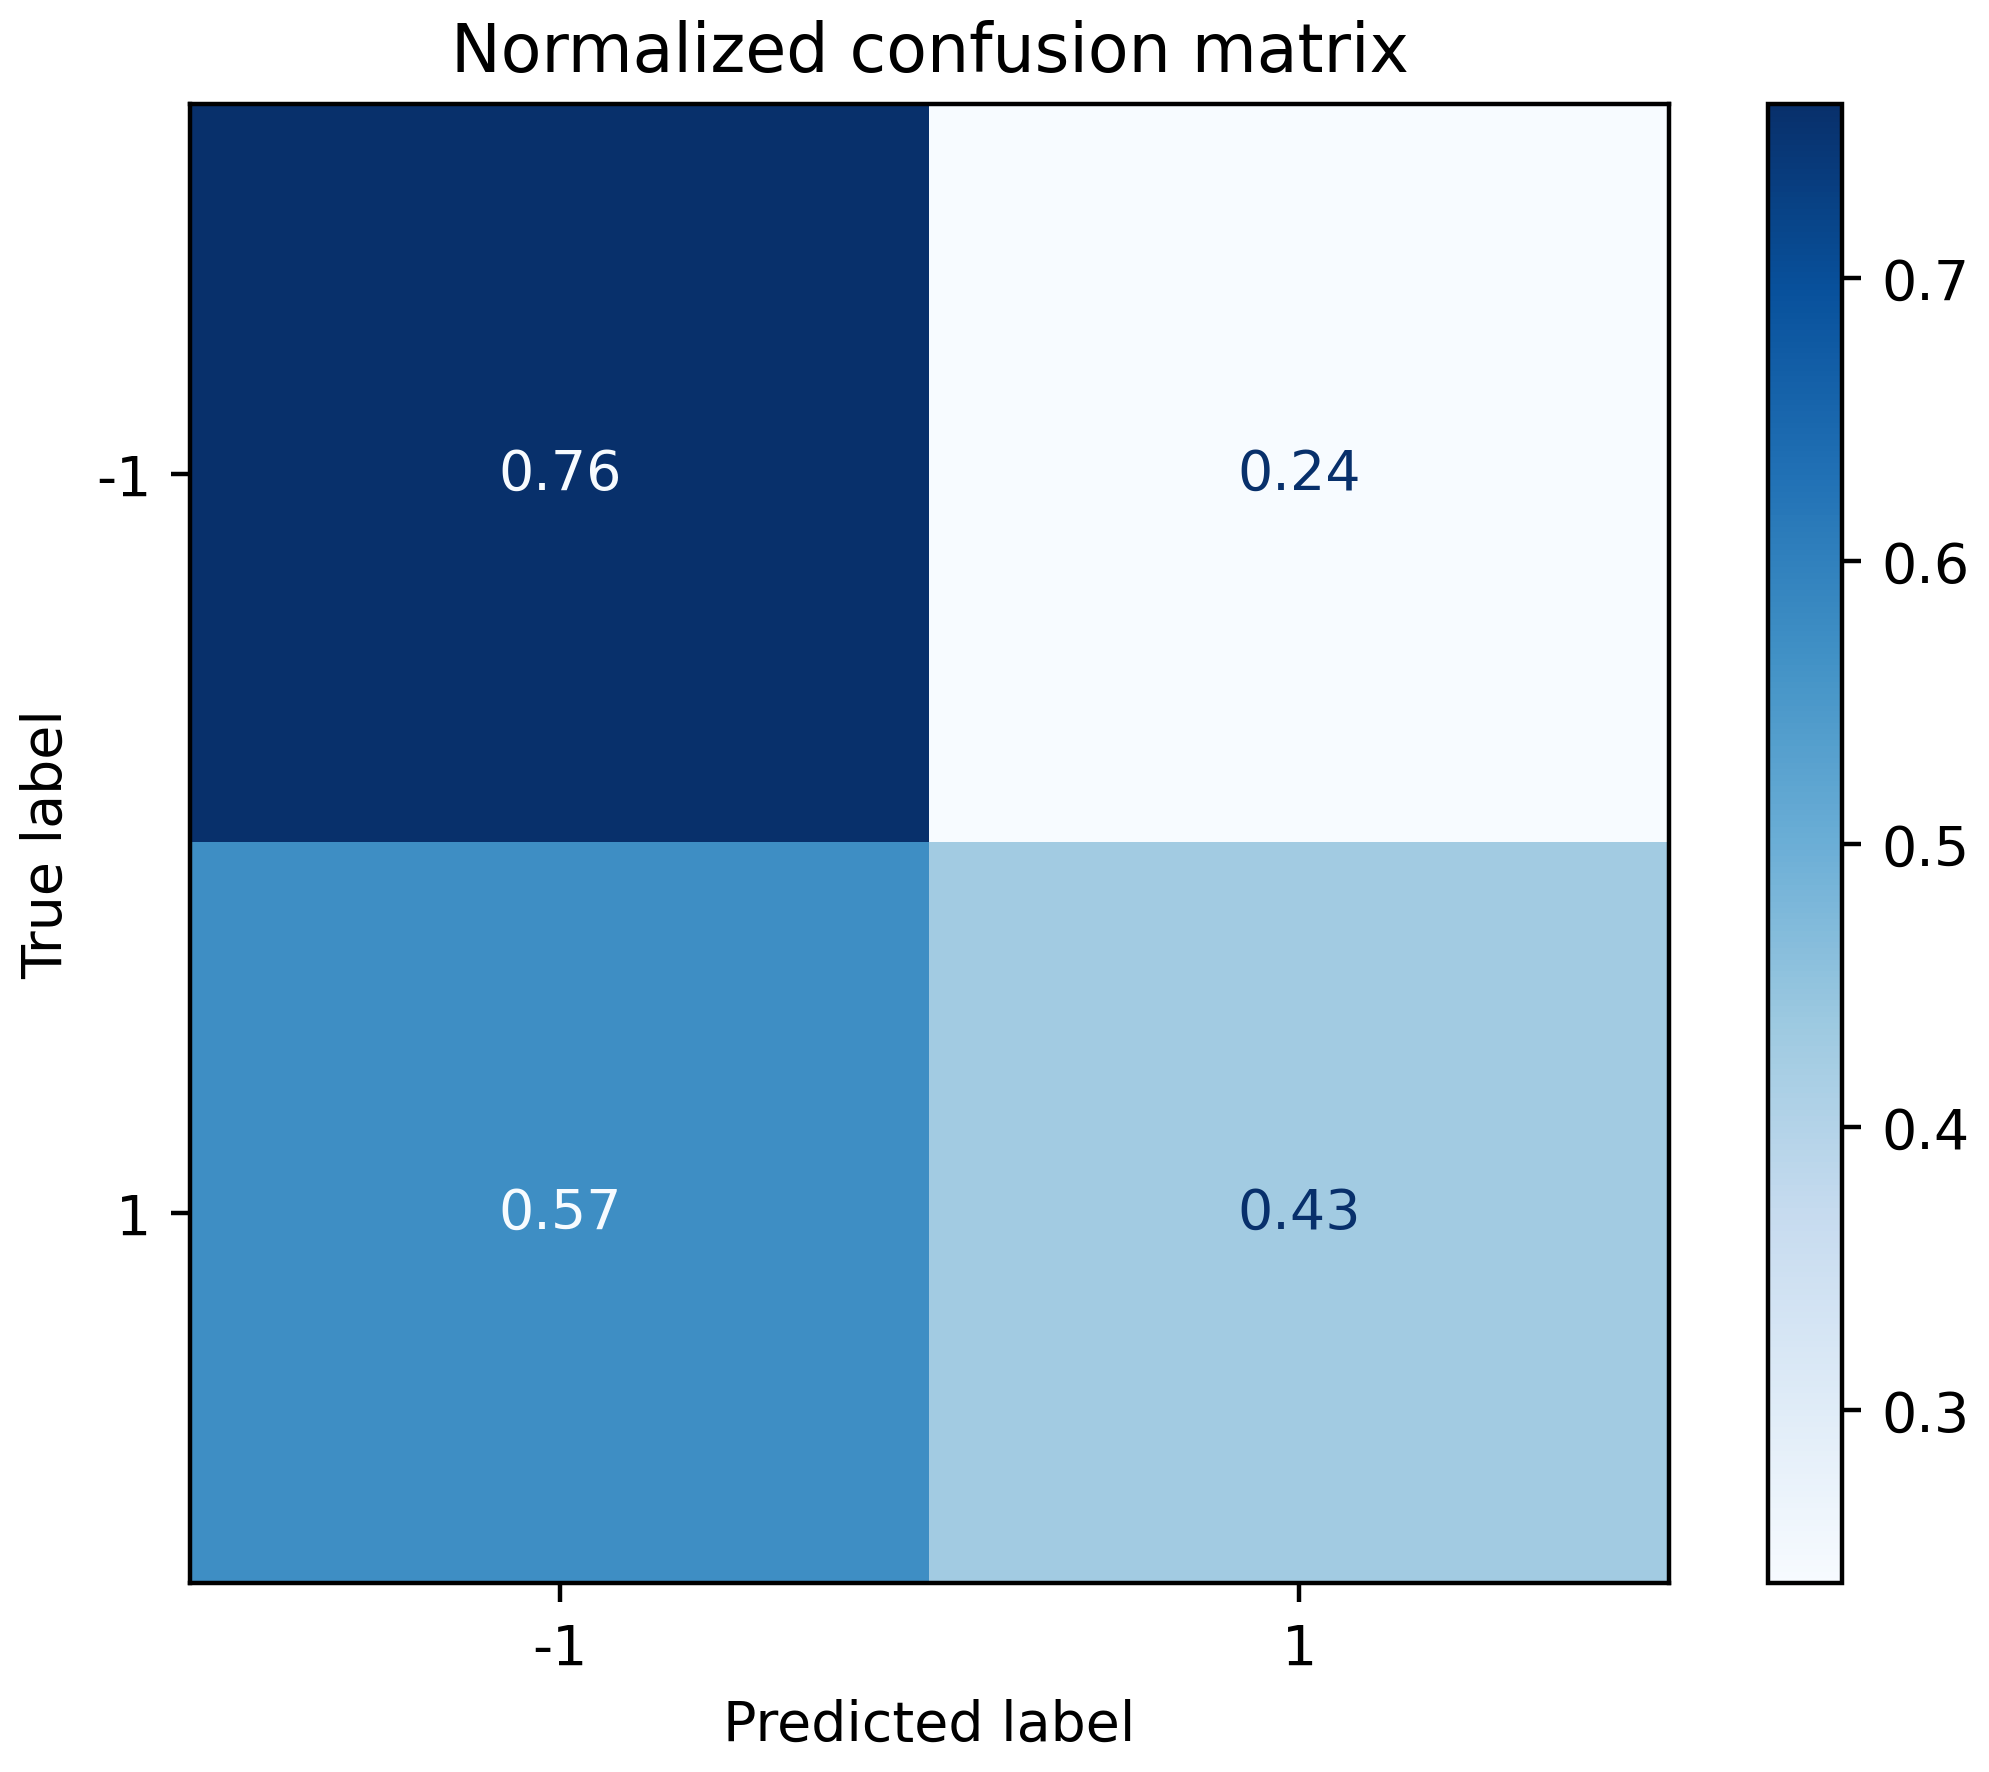
\includegraphics[width=0.48\linewidth]{KNN-re_confus_mat-norm.png}
%     \caption{使用SMOTE过采样和KNN的混淆矩阵(测试集)}
%     \label{fig:result:knn-re}
% \end{figure}

% \begin{figure}[!h]
%     \centering
%     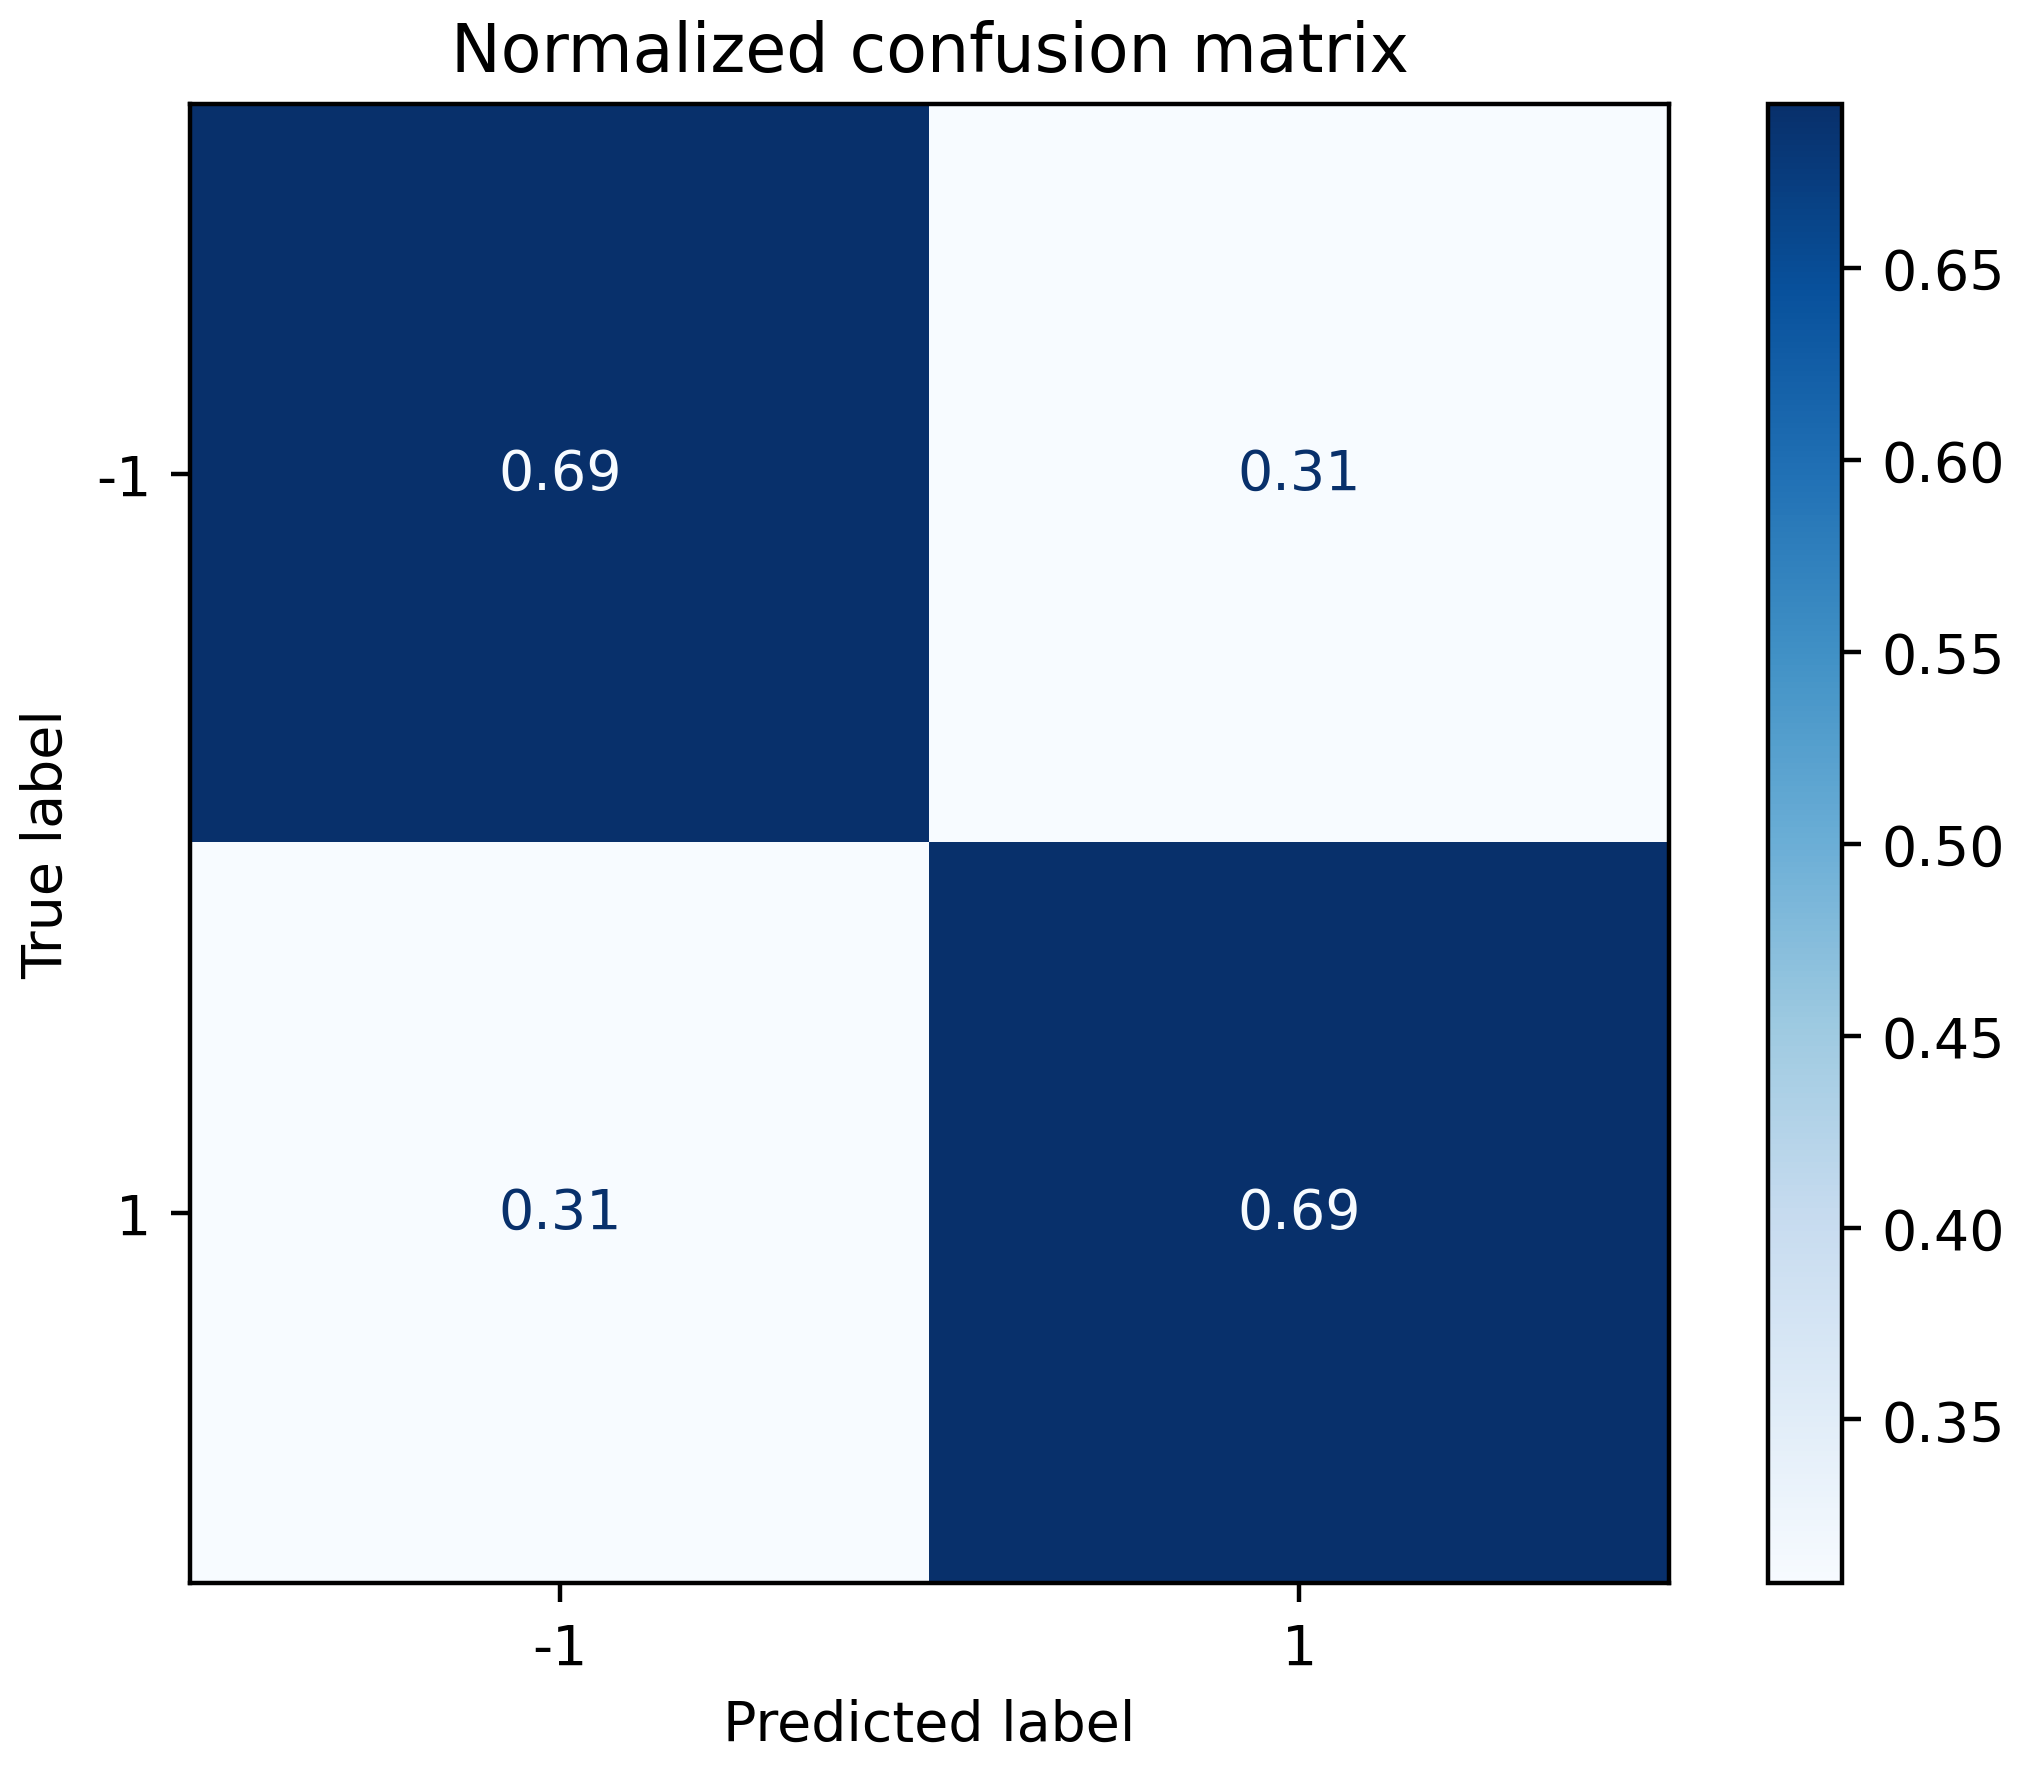
\includegraphics[width=0.48\linewidth]{AdaBoost-re_confus_mat-norm.png}
%     \caption{使用SMOTE过采样和AdaBoost的混淆矩阵(测试集)}
%     \label{fig:result:ada-re}
% \end{figure}

\begin{figure}[!h]
    \centering
    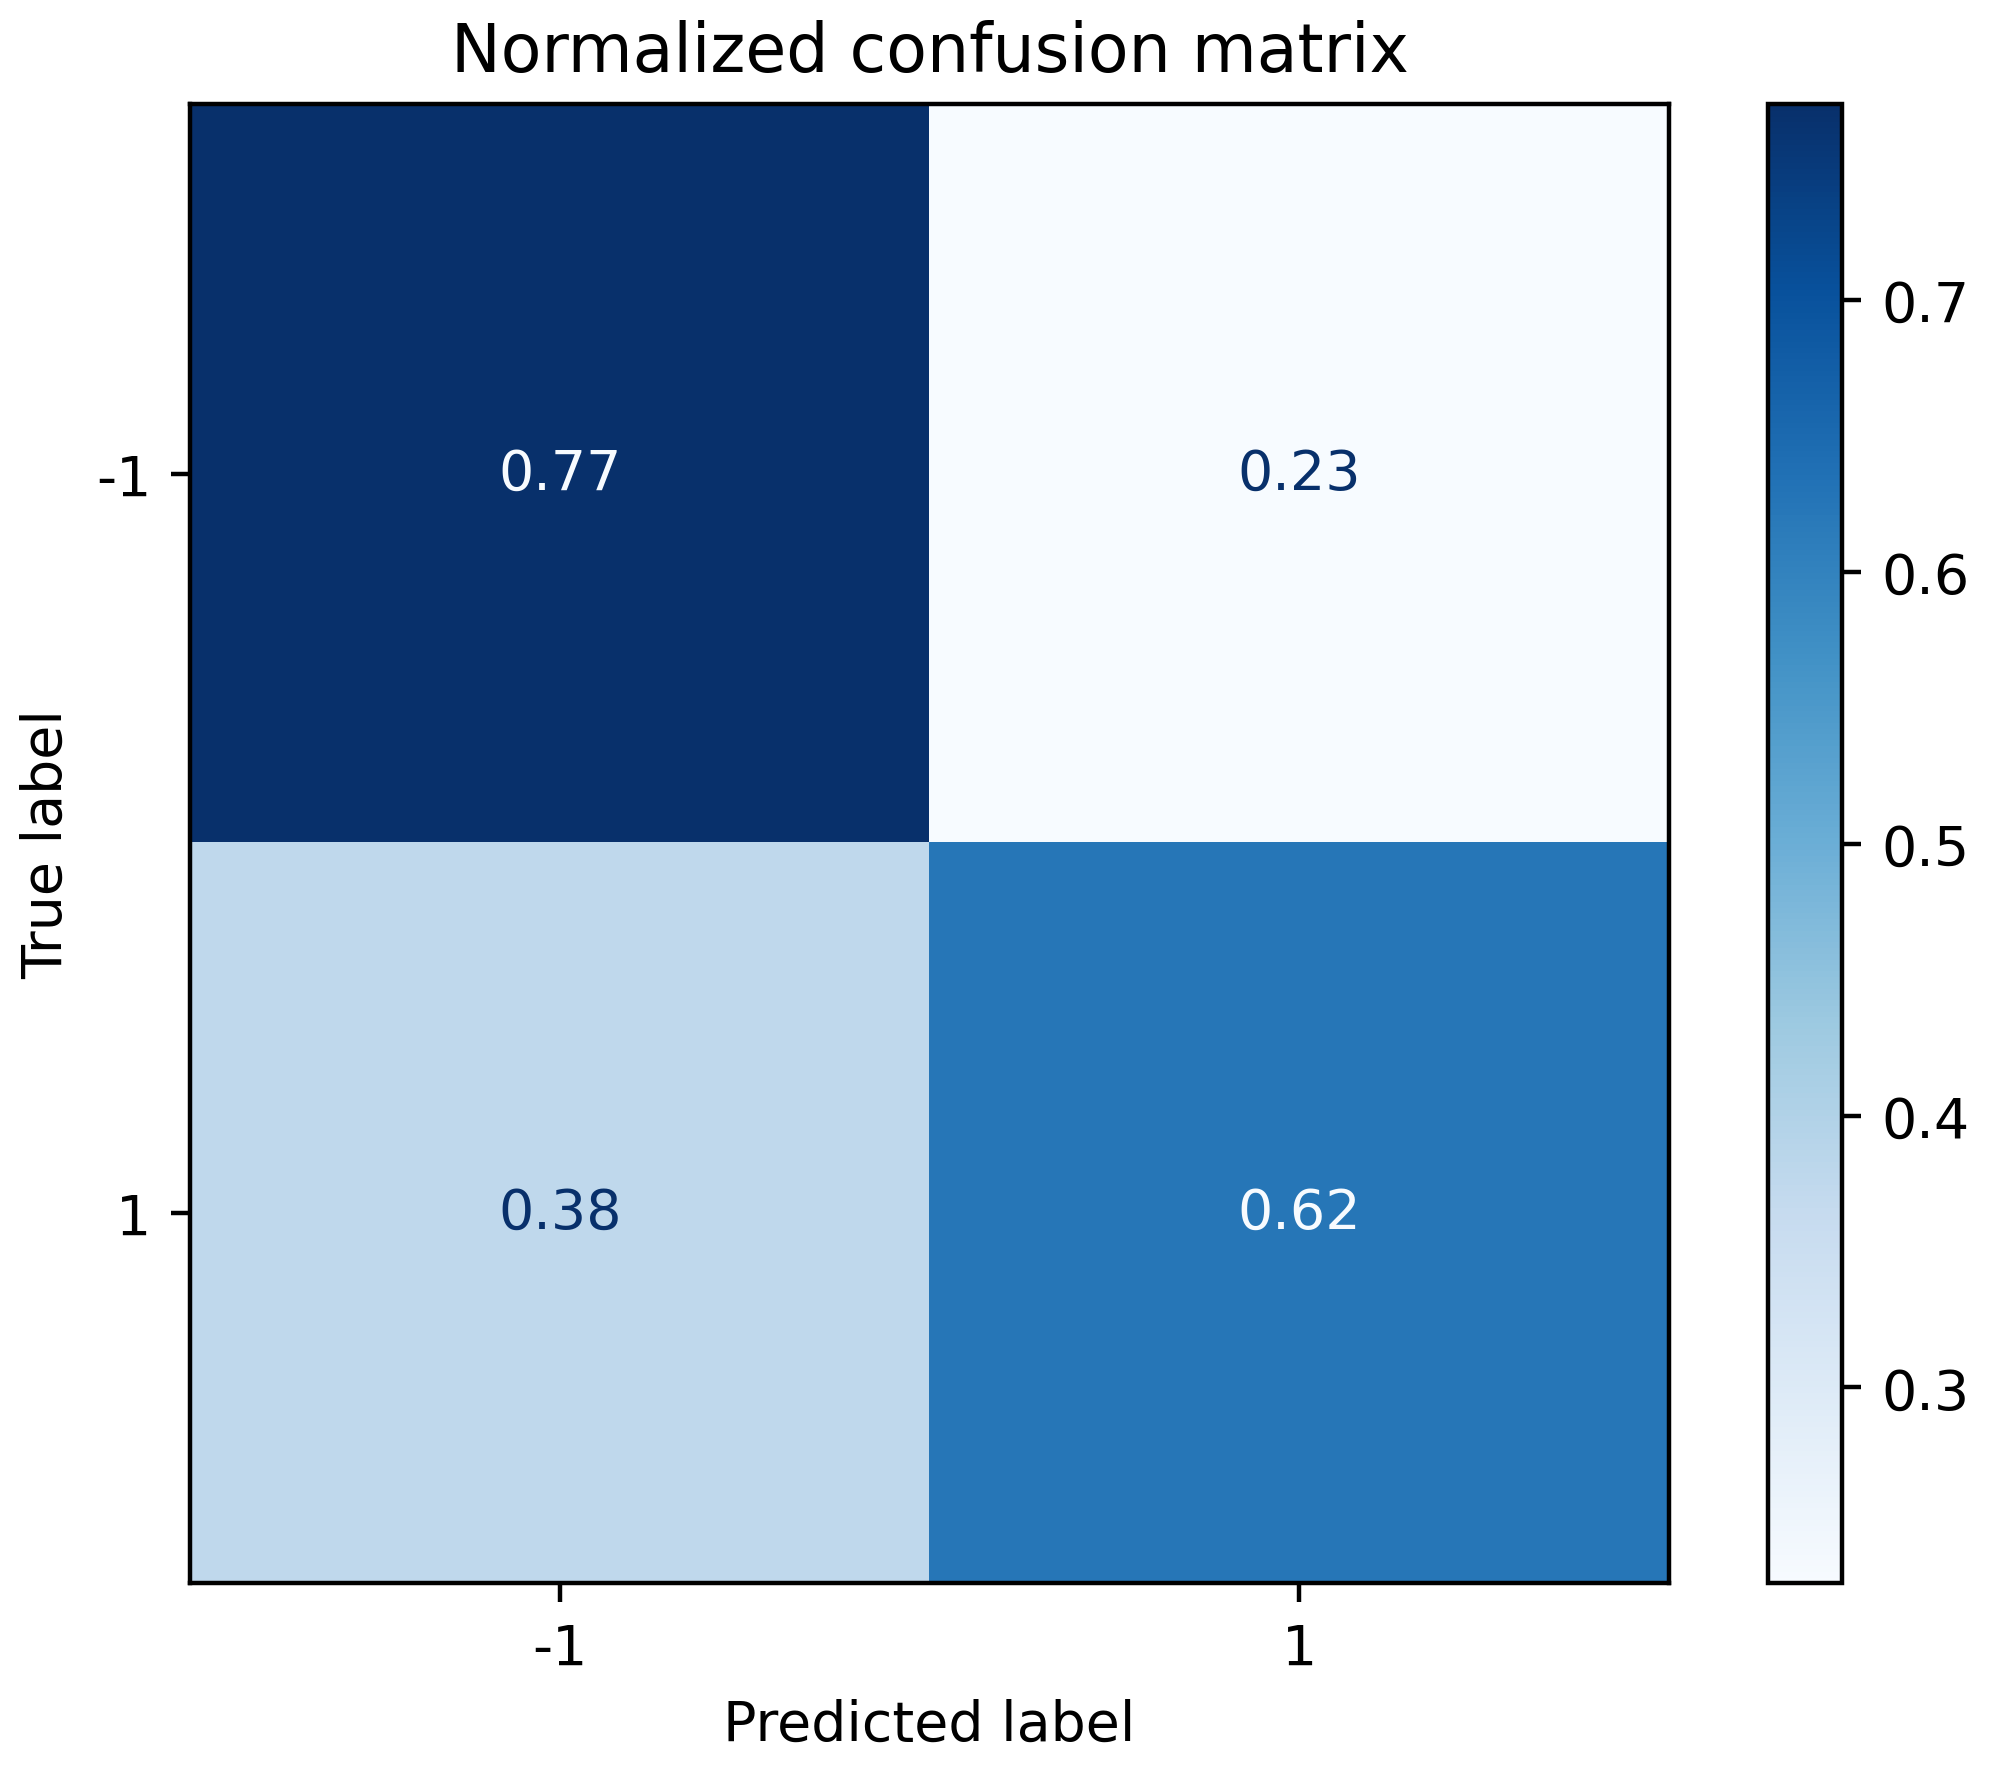
\includegraphics[width=0.48\linewidth]{GradientBoosting-re_confus_mat-norm.png}
    \caption{使用SMOTE过采样和GradientBoosting的混淆矩阵(测试集)}
    \label{fig:result:grad-re}
\end{figure}

同样,针对没有可选参数\texttt{class\_weight='balanced'}的模型 -- AdaBoost 和Gradient Boosting,都进行了实验查看过采样的影响,具有相似结果:AdaBoost 图\ref{fig:result:ada-re},Gradient Boosting 图\ref{fig:result:grad-re}。

\clearpage
\subsubsection{\texttt{class\_weight='balanced'} vs. 过采样}
% 所以比较 \texttt{class\_weight='balanced'} 参数和过采样的区别

进一步的,查看了\texttt{class\_weight='balanced'}的算法原理,是将不同样本数量的类,通过增加类权重,使得计算损失函数的时候,不同类的错误分类惩罚相同。
\begin{python}
from sklearn.utils.class_weight import compute_class_weight

class_weight = 'balanced'
label = [0] * 9 + [1]*1 + [2, 2] # 9个类0,1个类1,2个类2
print(label)  # [0, 0, 0, 0, 0, 0, 0, 0, 0, 1, 2, 2]
classes = [0, 1, 2]
weight = compute_class_weight(class_weight, classes, label)
print(weight)  # [ 0.44444444 4. 2. ]
print(.44444444 * 9)  # 3.99999996,类0
print(4 * 1)  # 4,类1
print(2 * 2)  # 4,类2
\end{python}

如上代码片段所示,可以看到 \texttt{class\_weight} 的调整是通过 \texttt{compute\_class\_weight} 这个函数把样本的平衡后的权重乘积(类样本数$\times$类权重)调整到同一值,每个类别均如此。因此,样本数少的类相对权重就越大,保证了损失函数不会因为样本不均衡而忽略样本少的类。

至于还有易于混淆的参数 \texttt{sample\_weight} 但是这参数目的目的不同,是为了调整样本采样时不同样本可信度的不同,导致需要在惩罚项上进行加权。\texttt{sample\_weight}是一个和长度为样本数量的向量,\texttt{class\_weight}是长度为类标签种数的向量。不过实际计算中 \texttt{Actual sample weights = sample\_weight *  class\_weight},如果没有\texttt{class\_weight} 或是设定为默认值,即\texttt{class\_weight=1} ,实际使用差异不大。

所以没有 \texttt{class\_weight='balanced'} 的参数设定,一样可以进行手动的样本过采样即可达到类似或等价的平衡效果。

% -----------------------------------Appendix----------------------------------------
% \appendix
% 这里附录


% \newpage
% -----------------------------------REFERENCE----------------------------------------
\bibliographystyle{acm}
\bibliography{main}

\end{document}

